\documentclass[5p,times]{elsarticle}

% The following \documentclass options may be useful:

% preprint      Remove this option only once the paper is in final form.
% 10pt          To set in 10-point type instead of 9-point.
% 11pt          To set in 11-point type instead of 9-point.
% numbers       To obtain numeric citation style instead of author/year.

\usepackage{amsmath}
\usepackage{mathtools}
\usepackage{graphicx}
\usepackage{listings}
\usepackage{color}
\usepackage{xcolor}
\usepackage{amsmath}
\usepackage{semantic}
\usepackage{url}
\usepackage{natbib}
\bibliographystyle{plainnat}
\usepackage[utf8]{inputenc}
\usepackage[english]{babel}
\usepackage{stmaryrd}
\usepackage{pgf}
\usepackage{caption}
\usepackage{subcaption}
\usepackage{multicol}
\usepackage{wasysym}
\usepackage{tikz}
\usepackage{amssymb}
\usepackage{graphicx}
\usepackage{epstopdf}
\usepackage{enumitem}
\usepackage{tocloft}
\usepackage{setspace}
\usepackage{verbatim}

\setlength\cftparskip{-2pt}
\setlength\cftbeforesecskip{1pt}
\setlength\cftaftertoctitleskip{2pt}
\setcounter{tocdepth}{3}

\usetikzlibrary{matrix,arrows,decorations.pathmorphing}

\definecolor{keywords}{rgb}{0,0,200}
\definecolor{comments}{rgb}{0,0.5,0}
\definecolor{types}{rgb}{0.99,0.1,0.99}
\definecolor{strings}{rgb}{0.5,0,0}

\def\figfontsize{\fontsize{6}{7}}

\lstdefinelanguage{ESL}{
         basicstyle=\footnotesize\ttfamily, % Standardschrift
         numbersep=5pt,              % Abstand der Nummern zum Text
         tabsize=1,                  % Groesse von Tabs
         extendedchars=true,         %
         breaklines=true,            % Zeilen werden Umgebrochen
         morecomment=[l]{//},
         columns=fullflexible,
         aboveskip=2mm,
         belowskip=2mm,
         frame=tb,
         stringstyle=\color{strings},
         commentstyle=\color{comments}, % style of comments
         keywordstyle=[1]{\ttfamily\color{keywords}}, 
         keywords=[1]{grab,or,case,for,null,data,if,else,new,type,probably,fun,set,bag,do,
                       fold,unfold,find,in,when,then,let,not,letrec,act,self,become,export,and,extends},
         keywordstyle=[2]{\ttfamily\color{types}}, 
         keywords=[2]{Act,Int,Bool,Str,Float,Array,Hash,Void,Fun,rec,Set,Bag,Forall,union},
         numbers=left,
         moredelim=[s][\color{strings}]{'}{'},
         moredelim= [s][\color{red}]{/*}{*/},
         escapeinside={(*}{*)},
         literate=%
           {...}{$\ldots$}{1}
           {::}{$\dblcolon$}{1}
           {->}{${\mathbin{\rightarrow}}$}1
           {<-}{$\leftarrow$}{1},
         showspaces=false,           % Leerzeichen anzeigen ?
         keepspaces=true,
         showtabs=false,             % Tabs anzeigen ? 
         showstringspaces=false      % Leerzeichen in Strings anzeigen ?        
 }

\lstnewenvironment{ESL} { \lstset{language=ESL} } { }

\lstnewenvironment{ESL*} { \lstset{language=ESL,frame=none} } { }

\lstnewenvironment{FigESL} { \lstset{language=ESL,frame=none,basicstyle=\figfontsize\ttfamily} } { }
  
\def\code#1{{\normalfont\lstinline[language=ESL,escapeinside={(*}{*)},basicstyle=\footnotesize\ttfamily]{#1}}}

\begin{document}

\begin{frontmatter}

%% Title, authors and addresses

\title{ESL Reference Guide}

\author{Tony Clark}

\address{Aston University, Birmingham, UK}

\begin{abstract}
ESL is an actor-based functional language that aims to provide abstractions over applications that require a high degree of concurrency. ESL is statically typed which means that programs can be verified for type safety before they run. ESL provides extensions over the standard Actor Model, including shared state and access to the underlying Java platform, for practical application development. ESL compiles to pure Java and runs against a small Java library. The ESL compiler is written in ESL. ESL is supported by a development environment called EDB that includes libraries for data visualisation in terms of HTML, SVG and GraphViz. This report provides a reference for ESL and EDB using examples.
\end{abstract}

\end{frontmatter}

%\maketitle

\tableofcontents

\section{Introduction}

\label{sec:introduction}

This document describes the language ESL and its implementation. ESL is an actor-based language that has been designed to offer a convenient way to build applications that benefit from a large number of independent concurrent processes that communicate in terms of structured data. ESL compiles directly to Java source code and can therefore easily integrate with Java applications. The benefit of using ESL compared to Java is the abstraction that it provides over the construction and management of processes and the data that is passed between them. In addition, ESL enforces a separation of concerns since communication is by asynchronous message which reduces the risks associated with large scale concurrency due to race conditions and shared data. Having said that, whilst ESL actors are encapsulated, it is unreasonable to build a large scale system without some degree of shared data, so ESL provides mechanisms for data sharing where needed. ESL aims to support system verification through an expressive statically checked type system.

\begin{figure}
\centering
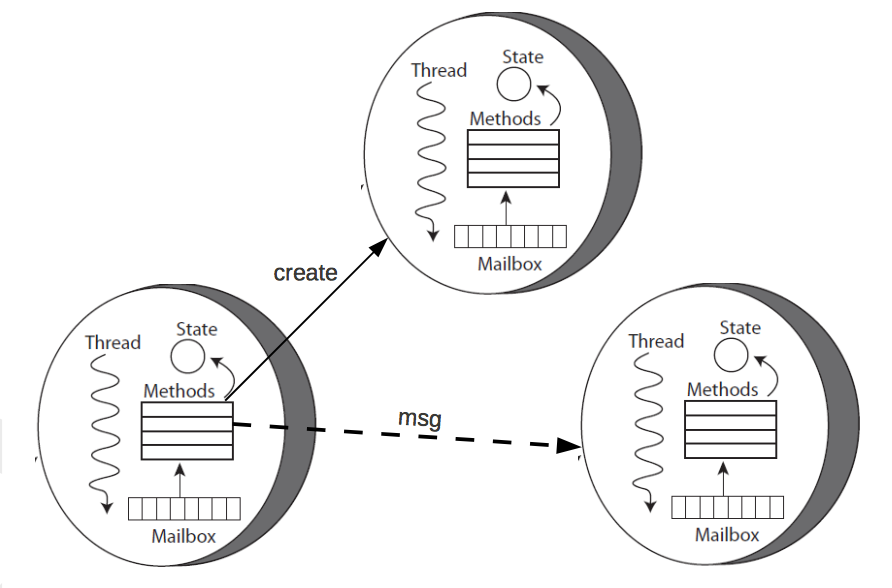
\includegraphics[width=\columnwidth]{actors}
\vspace{-0.20cm}
\caption{Actor Model of Computation \cite{karmani2009actor}}
\label{fig:actors}
\end{figure}

The Actor Model of Computation is characterised in figure \ref{fig:actors} which shows three actors. Each actor has a local thread of control which selects a message from the head of the mailbox and processes it. When the current message is processed, the thread inspects the mailbox for the next message; if no message is available then the actor becomes idle until a message is received. Each actor has a local state that can be inspected and updated by the methods that handle the messages.

An actor can send messages to any actor that it knows about. An actor will know about an actor if it created the actor or it received the actor as part of a message. A message may contain basic data items, collections of data item, actors, and functions. When a source actor passes a function to a target actor, the source may provide access to its internal state when the target calls the function on its own thread.

%%% Motivation for ESL

%%%The Actor Model

%%%Document Guide

\section{Data and Types}

\label{sec:data}

ESL provides basic data types: integers, floats, booleans and strings. For example the following listing declares identifiers along with their values. Comments follow the Java format:
\begin{ESL}
/* The parameters of the program are defined below.
   Change the starting position to get a different
   configuration. */
   
x::Int         = 100;     // Starting x position.
y::Int         = 200;     // Starting y position.
pi::Float      = 3.14;    // Used for position calculation.
isActive::Bool = true;    // True when moving.
name::Str      = 'Wilma'; // Used as a unique identifier.
\end{ESL}
Characters such as \code{#a} and \code{#+} are represented as integers ascii codes and are therefore of type \code{Int}. Special characters are introduced using \code{#\\} followed by their name: \code{#\\space}, \code{#\\newline} and \code{#\\backslash}.

ESL supports homogeneous arrays, for example the following is a one-dimensional array of strings with 100 elements indexed from 0:
\begin{ESL}
names::Array[Str] = new Array[Str](100);
names[0] := 'Wilma';
print[Str]('value at 0 = ' + names[0]);
\end{ESL}
Arrays may be nested, for example to create a two-dimensional array of booleans:
\begin{ESL}
points::Array[Array[Bool]] = new Array[Array[Bool]](100);
for x::Int in 0..100 do {
  points[x] := new Array[Bool](200);
  for y::Int in 0..200 do {
    points[x][y] := true;
  }
}
\end{ESL}
Note that array elements can be updated and passed between actors, therefore they are a basis for race conditions and other concurrency problems. The intention is that arrays are used locally within an actor as efficient indexable storage. If arrays are shared then access should be protected using locks.

ESL provides homogeneous lists whose elements cannot be modified by side effect and are therefore safe to pass between actors. A list is constructed using \code{::} and \code{[ ... ]} and can be decomposed using the operations \code{head} and \code{tail} in addition to pattern matching (see below). For example:
\begin{ESL}
nums::[Int] = [1,2,3,4,5,6,7,8,9,0];
print[Int](head[Int](nums));
print[[Int](tail[Int](nums))
print[[Int]](head[Int](nums) : tail[Int](tail[Int](nums));
\end{ESL}
which produces \code{1}, \code{[2,3,4,5,6,7,8,9,0]} and \code{[1,3,4,5,6,7,8,9,0]} respectively. Note that the operations \code{head} and \code{tail} are supplied with the type of the list element; this is because there operations are {\it polymorphic} as described in section \ref{sec:polymorphism}. The definition of \code{nums} above is equivalent to:
\begin{ESL}
nums::[Int] = 1:2:3:4:5:6:7:8:9:0:[];
\end{ESL}
Sets and bags are like lists except the elements are not ordered. Adding an element to a set or bag produces a new set or bag respectively. Adding an element to a set has no effect if the set already contains the element, otherwise both the set and bag are extended:
\begin{ESL}
setOfNames::Set{Str} = Set{'Fred','Wilma'};
bagOfNames::Bag{Str} = Bag{'Fred','Wilma'};
print[Set{Str}](Set{'Fred' | setOfNames});
print[Bag{Str}](Bag{'Fred' | setOfNames});
\end{ESL}
produces \code{Set\{'Fred','Wilma'\}} and \code{Bag\{'Fred','Wilma','Fred'\}} respectively. Note that extraction from sets and bags occurs via pattern matching is described below.
\begin{figure*}
\centering
\begin{tabular}{|c|c|}
\hline
{\bf Type}&{\bf Equality for Values of Type}\\\hline\hline
\code{i1,i2::Int} & \code{i1} and \code{i2} are the same number\\\hline
\code{f1,f2::Float} & \code{f1} and \code{f2} are the same number\\\hline
\code{s1,s2::Str} & \code{s1} and \code{s2} have the same characters in order\\\hline
\code{b1,b2::Bool} & \code{b1} and \code{b2} are the same boolean values\\\hline
\code{h1:l1,h2:l2::[T]} & \code{h1} is equal to \code{h2}, and \code{l1} is equal to \code{l2}\\\hline
\code{[]::[T]}&equal to an empty list of the same type.\\\hline
\code{set\{e1::T | s1::Set\{T\}\} set\{e2::T | s2::Set\{T\}\}} & \code{e1} and \code{e2} are equal, and \code{s1} and \code{s2} are equal\\\hline
\code{set\{\}::Set\{T\}}&is only equal to an empty set of the same type.\\\hline
\code{bag\{e1::T | b1::Bag\{T\}\} bag\{e2::T | b2::Bag\{T\}\}} & \code{e1} and \code{e2} are equal, and \code{b1} and \code{b2} are equal\\\hline
\code{bag\{\}::Bag\{T\}}&is only equal to an empty bag of the same type.\\\hline
\code{a1,a2::Array[T]} & \code{a1} and \code{a2} are the same array\\\hline
\code{t1,t2::Hash[K,V]} & \code{t1} and \code{t2} are the same table\\\hline
\code{a1,a2::Act \{...\}} & \code{a1} and \code{a2} are the same actor\\\hline
\code{f1,f2::(T ...) -> T} & \code{f1} and \code{f2} are the same function\\\hline
\code{r1,r2::\{ n->T ... \}}& \code{r1.n} is equal to \code{r2.n} for all names\\\hline
\code{C(n1,...), C(m2,...)}& equal when corresponding \code{ni} and \code{mi} are equal\\\hline
\code{null[T]} & only equal to the value null\\\hline
\end{tabular}
\caption{Data Equality}
\label{fig:data_equality}
\end{figure*}
Sets require a definition of equality for ESL values which is provided in figure \ref{fig:data_equality}.

ESL hash tables map keys to values. A hash table provides operations for adding a mapping, accessing the value for a key, testing whether a mapping exists. A hash table uses field reference to get the list of keys and the list of values:
\begin{ESL}
ages::Hash[Str,Int] = new Hash[Str,Int];
ages.put('Fred',35);
ages.put('Wilma',32);
print[Bool](ages.hasKey('Fred'));
print[Int](ages.get('Wilma'));
print[[Str]](ages.keys);
print[[Int]](ages.vals);
\end{ESL}
prints \code{true}, \code{32}, \code{[Fred,Wilma]}, and \code{[35,32]}. Note that because hash tables are updated by side effect, they are not thread safe and should be used locally within an actor, or access should be protected using locks.

ESL functions are first-class values and may be passed between actors within data structures. The rules for identifier binding within functions are defined in section \ref{sec:binding}. A simple example of a function is:
\begin{ESL}
add1::(Int)->Int = fun(x::Int)::Int x + x;
print[Int](add1(100));
\end{ESL}
which prints \code{101}.

Records map names to values. Unlike hash tables, the domain of a record is fixed. New type names can be defined that refer to existing types, so the following code implements an two-dimensional point object:
\begin{ESL}
type Point = { x::Int; y::Int }
mkPoint(n::Int,m::Int)::Point = {x->n; y->m}
print[Point](mkPoint(100,200));
print[Int](mkPoint(100,200).x);
\end{ESL}
prints \code{\{x=100,y=200\}} and \code{100}. Records cannot be updated by side effect.

The value \code{null} can be used as an undefined value for any data type. It is polymorphic and is followed by the type for which it acts as undefined. For example:
\begin{ESL}
x::Int = null[Int];
p::Point = null[Point];
\end{ESL}
The following operations are builtin to ESL:
\begin{ESL}
_ + _       :: (Int,Int)       -> Int      // addition
_ + _       :: (Float,Float)   -> Float    // addition
_ + _       :: (Str,T)         -> Str      // concatenation
_ + _       :: (T,Str)         -> Str      // concatenation
_ + _       :: ([T],[T])       -> [T]      // concatenation
_ + _       :: (Set{T},Set{T}) -> Set{T}   // union
_ - _       :: (Int,Int)       -> Int      // subtraction
_ - _       :: (Float,Float)   -> Float    // subtraction
_ * _       :: (Int,Int)       -> Int      // multiplication
_ * _       :: (Float,Float)   -> Float    // multiplication
_ / _       :: (Int,Int)       -> Int      // division
_ / _       :: (Float,Float)   -> Float    // division
_ % _       :: (Int,Int)       -> Int      // modulo
_ = _       :: (T,T)           -> Bool     // equal to
_ <> _      :: (T,T)           -> Bool     // not equal to
_ and _     :: (Bool,Bool)     -> Bool     // boolean and
_ or _      :: (Bool,Bool)     -> Bool     // boolean or
not         :: (Bool)          -> Bool     // boolean not
_ .. _      :: (Int,Int)       -> [Int]    // integer range
_ @ _       :: (T,T)           -> T        // parallel
print[T]    :: (T)             -> Void     // print 
random      :: (Int)           -> Int      // random value
wait        :: (Int)           -> Void     // thread delay
isqrt       :: (Int).          -> Float    // square root
intToFloat  :: (Int)           -> Float    // conversion
round       :: (Float)         -> Int      // conversion
stopAll     :: ()              -> Void     // halt execution
\end{ESL}
When an ESL identifier is defined its type must be declared. Types are defined as follows:
\begin{center}
\footnotesize
\begin{tabular}{|c|c|}
\hline
{\bf Type}&{\bf Description}\\\hline\hline
\code{Int}&integers\\\hline
\code{Float}&floats\\\hline
\code{Bool}&booleans\\\hline
\code{Str}&strings\\\hline
\code{Void}&nothing\\\hline
\code{[T]}&lists\\\hline
\code{(T,...) -> T}&functions\\\hline
\code{Array[T]}&arrays\\\hline
\code{Set\{T\}}&sets\\\hline
\code{Bag\{T\}}&bags\\\hline
\code{Hash[T,T]}&hash tables\\\hline
\code{\{i:T;...\}}&records\\\hline
\code{Forall[V,...] T}&polymorphic values\\\hline
\code{rec V. T}&recursive types\\\hline
\code{union \{ C(T,...);... \}}&union types\\\hline
\end{tabular}
\end{center}
A type may be named and then the name can be used as a shorthand. For example:
\begin{ESL}
type Ints    = [Int];
type AddInts = (Ints,Ints) -> Ints;

addInts::AddInts = fun(l1::Ints,l2::Ints)::Ints 
  case l1,l2 {
    [],l -> [];
    l,[] -> [];
    x:l1,y:l2 -> (x+y):addInts(l1,l2);
  }
\end{ESL}
A function binding can be defined in-line so that the example above can be expressed as follows:
\begin{ESL}
addInts(l1::Ints,l2::Ints)::Ints =
  case l1,l2 {
    [],l -> [];
    l,[] -> [];
    x:l1,y:l2 -> (x+y):addInts(l1,l2);
  }
\end{ESL}
Types can be recursive, for example the following implements two dimensional points with function updates:
\begin{ESL}
type Point2D = {
  getX::()->Int;
  getY::()->Int;
  setX::(Int)->Point2D;
  setY::(Int)->Point2D
};

mkPoint(x::Int,y::Int)::Point2D = {
  getX -> fun()::Int x;
  getY -> fun()::Int y;
  setX -> fun(x::Int)::Point2D mkPoint(x,y); 
  setY -> fun(y::Int)::Point2D mkPoint(x,y) 
};

let p::Point2D = mkPoint(100,200);
in {
  print[Int](p.getX());
  print[Int](p.setX(p.getX()+1).getX());
}
\end{ESL}
which prints \code{100} then \code{101}.

\section{Blocks and Commands}

\label{sec:commands}

The type \code{Void}, like Java, represents an evaluation that does not return a result. The operation \code{print[T](t)} takes a value \code{t::T} and `returns' \code{Void}. A {\it block} is a sequence of {\it commands} enclosed in curly brackets. A command is just any expression, but syntactically, if the expression does not end with a closing \code{\}}, then the command must be terminated with a semicolon. The return value of a block is the return value of the last command. For example:
\begin{ESL}
print3(a::Int,b::Int,c::Int)::Void = {
  print[Int]('first = ' + a);
  print[Int]('second = ' + b);
  print[Int]('third = ' + b);
}
\end{ESL}
The special case of the block \code{\{\}} is of type \code{Void}.

\section{List Comprehensions and List Operations}

\label{sec:cmp}

Lists are a very useful way of organising collections of elements. They can easily be processed using recursion because of their structure: a list is either empty \code{[]} or is a list \code{l} with a head element \code{e} `consed' to the tail: \code{e:l}. 

A {\it list comprehension} is an expression that transforms lists. It has the form: 
\code{[ e | q ... ]}
where \code{e} is an expression and \code{q} is a {\it qualifier}. The idea is that a list is constructed whose elements are formed by evaluating \code{e} after performing each of the qualifiers in turn. There are two types of qualifier: {\it binding} and {\it predicate}. A binding qualifier has the form \code{p <- e} where \code{p} is a pattern and \code{e} is an expression whose value is a list. When it is evaluated, a binding qualifier repeatedly matches the elements from the list against the pattern. A predicate qualifier has the form \code{?e} where \code{e} is a boolean valued expression. When it is evaluated, if the expression in a predicate qualifier produces \code{true} then execution continues, otherwise it ignores the element most recently selected by a binding qualifier and selects the next element. For example:
\begin{ESL}
[ n | n <- 0..100, ?(n % 2 = 0) ]
\end{ESL}
produces a list of even numbers between \code{0} and \code{99} inclusive. Multiple binding qualifiers may be used:
\begin{ESL}
[ mkPoint(x,y) | x <- 0..100, y <- 0..200, ?(x <> y) ]
\end{ESL}
Lists can be processed using recursive functions and pattern matching. Typically a case-expression is used to match against a base case (often \code{[]}) and a recursion case (often \code{h:t}). For example the following operation adds up the distances of all points to the origin:
\begin{ESL}
addDists(ps::[Point])::Float =
  case ps {
    [] -> 0.0;
    h::t -> distanceToOrigin(h) + addDists(t);
  }
\end{ESL}
The following defines Quicksort in ESL:
\begin{ESL}
qsort(l::[Int])::[Int] =
  case l {
    [] ->[];
    x:l ->
      qsort([ n | n <- l, ?(n<x) ])
      + [x] +
      qsort([ n | n <- l, ?(n>x) ]);
  }
\end{ESL}
The collection of list operations that are supported by ESL are shown in \ref{sec:list_operations}.

\section{Algebraic Data Types and Pattern Matching}

ESL supports algebraic data types, also known as {\it union types}. For example, the directions of the compass can be represented using different integers or strings, but it is better to define a new type \code{Direction} and to have 4 unique values of that type. This can be defined as follows:
\begin{ESL}
data Direction =
  North
| South
| East
| West;
\end{ESL}
Now any identifier defined to have type \code{Direction} can hold one of the 4 values and the special value \code{null[Direction]}:
\begin{ESL}
d::Direction = North;
\end{ESL}
Pattern matching can be used with such a data type:
\begin{ESL}
moveRight(dir::Direction)::Direction =
  case dir {
    North -> East;
    East  -> South;
    South -> West;
    West  -> North;
  }
\end{ESL}
Given a list of such directions, they can be mapped:
\begin{ESL}
dirs::[Direction] = [ North, South, East, West ];
[ moveRight(d) | d <- dirs ]
\end{ESL}
The element types of a union can have components. For example a tree of integers:
\begin{ESL}
data TreeOfInt = 
  Branch(TreeOfInt,TreeOfInt)
| Leaf(Int);
\end{ESL}
Note that a branch term contains two integer trees and a leaf contains an integer. The integers in the tree can be added together:
\begin{ESL}
addTreeOfInt(t::TreeOfInt)::Int =
  case t {
    Branch(l,r) -> addTreeOfInt(l) + addTreeOfInt(r);
    Leaf(n)     -> n;
  }
print[Int](addTreeOfInt(Branch(Leaf(100),Leaf(200))));
\end{ESL}
Prints \code{300}. When pattern matching, the case arms are tried in turn, so we can define a short-cut version:
\begin{ESL}
addTreeOfInt(t::TreeOfInt)::Int =
  case t {
    Branch(Leaf(0),t) -> addTreeOfInt(t);
    Branch(t,Leaf(0)) -> addTreeOfInt(t);
    Branch(l,r)       -> addTreeOfInt(l) + addTreeOfInt(r);
    Leaf(n)           -> n;
  }
\end{ESL}
Case arms may contain conditions. For example, adding up all those elements of a tree that satisfy a predicate:
\begin{ESL}
addIf(p::(Int)->Bool,t::TreeOfInt)::Int =
  case t {
    Branch(l,r)       -> addIf(p,l) + addIf(p,r);
    Leaf(n) when p(n) -> n;
    Leaf(n)           -> 0;
  }
addIf(fun(n::Int)::Bool n > 100,Branch(Leaf(100),Leaf(200)));
\end{ESL}
Prints \code{200}.

\section{Sets and Collection Matching}

\label{sec:sets}

ESL supports homogenous sets: the empty set \code{set\{\}}; a set constructed from an element \code{e} and a set \code{s}, \code{set\{e | s\}}; a set union \code{s1 + s2}. Both sets and lists can be processed using pattern matching. For example:
\begin{ESL}
setContainsInt(s::Set{Int},x::Int)::Bool =
  case s {
    set{y | z} when x = y -> true;
    s                     -> false;
  }
\end{ESL}
The operation \code{setContainsInt} uses pattern matching to select the element \code{y} which is equal to the argument \code{x}. Note that sets are unordered, so the pattern \code{set\{y | z\}} is {\it non-deterministic}. When  the supplied value \code{s} matches the pattern, one of the elements in the set is matched against \code{y}; if the pattern fails to match before the corresponding \code{->} then a different element \code{y} will be chosen. In the example, the condition \code{x = y} is within the scope fo the choice, this causes elements from the set \code{s} to be tried un turn until one that matches \code{x} is found or the set is exhausted. If all the values have been tried from the set \code{s} then the case-arm fails and the next case-arm is tried.

Non-deterministic choice may occur more than once in the same pattern. For example, the following returns a duplicate entry in two sets:
\begin{ESL}
duplicate(s1::Set{Int},s2::Set{Int},notFound::Int)::Int =
  case s1,s2 {
    set{x | p}, set{y | q} when x = y -> x;
    s1,s2                             -> notFound;
  }
\end{ESL} 
The first case-arm in \code{duplicate} selects an element \code{x} from \code{s1}, then selects \code{y} from \code{s2} such that they are equal elements. If there is no element in common then the \code{notFound} element is returned.

Non-deterministic pattern-based choice can be used over lists using the pattern \code{p1 + [p2] + p3} where \code{p1} matches a prefix of a list, \code{p2} matches some element, and \code{p3} matches a suffix. The pattern fails in the case that the list if empty. For example, testing whether a given element occurs in a list:
\begin{ESL}
intMember(n::Int,l::[Int])::Bool =
  case l {
    l1 + [x] + l2 when x = n -> true;
    l                        -> false;
  }
\end{ESL}

\section{Actors}

%%% Behaviour types, behaviours, new.

Actors are implemented in terms of {\it behaviour types} and {\it behaviours}. A behaviour type provides an interface definition for a set of behaviours. An interface consists of message types and exported identifiers and their types. Consider a simple behaviour type called \code{Sink} that accepts a single type of message \code{M(Int)}:
\begin{ESL}
Act Sink {
  M(Int);
}
\end{ESL}
Any behaviour of type \code{Sink} must implement the message \code{M}:
\begin{ESL}
act sink::Sink {
  M(n::Int) -> print[Str]('got: ' + n);
}
\end{ESL}
There can be any number of behaviours with the same type:
\begin{ESL}
act sink2::Sink {
  M(n::Int) -> {} // Ignore the message.
}
\end{ESL}
An actor is created with a specific behaviour:
\begin{ESL}
s::Sink = new sink;
\end{ESL}
Once created, the actor can receive messages. A message is asynchronous: \code{s <- M(100)} and is placed on the input queue of the target actor. Each actor is processing at most one message at any time, and is idle if there are no messages on its queue and it is not currently handling a message. Since all actors run concurrently, there is no guarantee that of message ordering other than messages sent from the same actor will retain the ordering in which they are sent.

Any number of behaviours can be defined to conform to a behaviour type. The following shows three different implementations of the type \code{A}. The first, \code{a}, just loops indefinitely which an actor can do because all message handling occurs concurrently with other actors. The second, \code{forward} is supplied with a second actor of type \code{A} to which it forwards messages. Finally, \code{broadcast} is supplied with a collection of actors of type \code{A} and will send any message to all of them:
\begin{ESL}
Act A {
  M(Int,Bool);
}

act a::A {
  M(n::Int,b::Bool) -> 
   self <- M(n,not(b));
}

actor::A = new a;

act forward(other::A)::A {
  M(n::Int,b::Bool) -> 
    other <- M(n,b);
}

proxy::A = new forward(actor);

act broadcast(as::[A])::A { 
  toAll(l::[A],n::Int,b::Bool)::Void =
    case l {
      [] -> {};
      h::A:t::[A] -> {
        h <- M(n,b);
        toAll(t,n,b);
      }
    }
  M(n::Int,b::Bool) ->
    toAll(as,n,b);
  } 

spray::A = new broadcast([new forward(new a) | i <- 0.1000]);

\end{ESL}

Often we want to do some initialisation when an actor is created. The special message handler \code{->} is run each time a new actor is created before any messages are processed:
\begin{ESL}
act sink3::Sink {
  -> print[Str]('I am initialising');
  M(n::Int) -> print[Str]('got: ' + n);
}
\end{ESL}
Actors can refer to other actors. The following pair of actors will bounce messages back and forth until the counter runs down:
\begin{ESL}
Act Ping {
  Ping(Int,Pong);
}

Act Pong {
  Pong(Int,Ping);
}

act ping::Ping {
  Ping(0,p::Pong)      -> print[Str]('stop');
  Ping(n::Int,p::Pong)  -> 
    p <- Pong(n-1,self);
}

act pong::Pong {
  Pong(0,p::Ping)      -> print[Str]('stop');
  Pong(n::Int,p::Ping)  -> 
    p <- Ping(n-1,self);
}

p1::Ping = new ping;
p2::Pong = new pong;
p1 <- ping(100,p2);
\end{ESL}
Behaviour definitions can be parameterised so that new actors can initialise the behaviour. For example, in order to provide an identifier to each actor. In the following example, we create a collection of machines and then broadcast jobs. A machine can process a job if the identifier matches:
\begin{ESL}
Act Machine {
  Process(Int);
}

act machine(id::Int)::Machine {
  Process(m::Int) when m = id -> {
    print[Str]('handling job');
  }
  Process(m::Int) -> {} // Ignore job if not target machine.
}

noOfMs::Int         = 100;
noOfJs::Int         = 10000;
machines::[Machine] = [ new machine(n) | n <- 0..noOfMs ];

for job::Int in 0..noOfJs do {
  let targetMachine::Int = random(noOfMs);
  in {
    for m::Machine in machines do {
      m <- Perform(targetMachine);
    }
  }
}
\end{ESL}
An actor may perform \code{become} to change behaviour. The replacement behaviour must implement the same behaviour type. Subsequent messages are handled by the new behaviour. For example, a resource manager allocates resource on request and becomes pending resource manager for the period of time when resources are unavialable:
\begin{ESL}
type Resource = ...;
Act Consumer {
  Receive(Resource);
}

Act ResourceManager {
  Allocate(Consumer);
  Free(Resource);
}

act manager(rs::[Resource])::ResourceManager {
  Allocate(c::Consumer) when rs = [] -> {
    become pending;
    self <- Allocate(c);
  }
  Allocate(c::Consumer) -> {
    become manager(tail[Resource](rs));
    c <- Receive(head[Resource](rs);
  }
  Free(r::Resource) -> become manager(r:rs);
}

act pending::ResourceManager {
  Allocate(c::Customer) -> self <- Allocate(c);
  Free(r::Resource) -> become manager([r]);
}
\end{ESL}

\section{Binding and Scope}

\label{sec:binding}

%%% Let , letrec, functions, locals in behaviours, state, update, functions. Loops.

ESL is a statically scoped language meaning that identifiers can be referenced within the textual binding block in which they are defined. Identifiers can be introduced as: function arguments; let-bindings; letrec-bindings; behaviour definitions; behaviour arguments (equivalent to function arguments); top-level definitions; pattern variables; for-loop controls. This section addresses each of these categories in turn.

Let-expressions introduce local bindings for the scope of the body of the let. A let-expression may have multiple bindings in which case they are performed in parallel:
\begin{ESL}
let dx::Int = x1-x2;
    dy::Int = y1-y2;
in isqrt((dx*dx)+(dy*dy));
\end{ESL}
A let-binding can be used to define a local function. Special syntax allows a function to be defined without using the keyword \code{fun}:
\begin{ESL}
let 
  distance(x1::Int,y1::Int,x2::Int,y2::Int)::Float =
    let dx::Int = x1-x2;
        dy::Int = y1-y2;
    in isqrt((dx*dx)+(dy*dy));
in distance(100,200,50,70);
\end{ESL}
A letrec-expression can be used to create local recursive functions:
\begin{ESL}
letrec 
  contains(l::[Int],n::Int)::Bool =
    case l {
      [] -> false;
      h:t when h=n -> true;
      h:t -> contains(t,n);
    }
in contains([1,2,3,4,5,6,7,8,9],5);
\end{ESL}
A letrec-expression can be used to create mutually recursive function definitions:
\begin{ESL}
letrec
  isEvan(n::Int)::Bool = if n = 0 then true else isOdd(n-1);
  isOdd(n::Int)::Bool = if n = 0 then false else isEven(n-1);
in isEven(101);
\end{ESL}
Letrec-bindings that do not establish functions are performed in sequence.

Behaviour definitions contain a collection of bindings that are established as a letrec and scoped over the message handlers of the behaviour. In addition, the names of local bindings can be exported and referenced using the \code{_._} operation. An an example, support we have a post office actor that delivers letters to people by matching up the address in the message:
\begin{ESL}
Act Person {
  export getAddress::()->Str;
}

act person(address::Str)::Person {
  export getAddress;
  getAddress()::Str = address;
  Open(Letter);
}

data Letter = Letter(Str,Str);

Act PostOffice {
  Deliver(Str);
}

act postOffice(people::[Person])::PostOffice {
  findPerson(address::Str,people::[Person])::Person =
    case people {
      [] -> throw[Person]('cannot deliver to ' + address);
      p:ps when p.getAddress() = address -> p;
      p:ps -> findPerson(address,people);
    }
  Deliver(Letter(name,address)) -> 
    findPerson(address) <- Open(Letter(name,address));
}
\end{ESL}

\section{Modules}

label{sec:modules}

ESL is a compiled language. The units of compilation are called modules and are usually contained in text files. A module contains a collection of mutually recursive bindings for types, behaviours, functions and values. A module \code{m} may export some of its bindings so that they can be used by any other module that imports \code{m}. For example a module defined in a file \code{a/b/c.esl} defines two names and exports one of them:
\begin{ESL}
export f;

f(n::Int)::Int = g(n) + 1;
g(n::Int)::Int = n + 100;
\end{ESL}
A second module can then import \code{c} and use the exported name:
\begin{ESL}
export main;

import 'a/b/c.esl';

g(n::Int)::Int = n = 200;

act Main::Act{} {
  -> print[Int](f(10));
}
\end{ESL}
prints 111. Note that the second module above defines a behaviour names \code{main}. When building an application there should be a root module that defines \code{main} which is the entry point for the application. When ESL starts to run a module it creates a single actor with the behaviour \code{main}. There is no restriction on the behaviour type of \code{main}.

\section{Time}

\label{sec:time}

ESL applications can be driven by a system clock. This can be useful when the application is driven by click ticks or when the application should run for a specific length of time. In order to receive clock ticks, a behaviour must implement at least one message handler of type \code{Time(Int)}. Any actor with such a behaviour will receive clock ticks {\it when the actor is idle}. If an actor does not define a handler for \code{Time{Int}} then there is no overhead for handling time.

The value of \code{n} in \code{Time(n)} is the time in milliseconds since the start of the application. The frequency of the ticks is undefined and therefore there is no guarantee that an actor will receive a tick with a specific value of \code{n}, and it may be the case the an actor receives multiple messages with the same value of \code{n}.

An actor may call \code{wait(n)} which causes the actor's thread to wait for \code{n} milliseconds. Since all actors have concurrent behaviours, a call of \code{wait} will not affect any other actor.

The following definition shows a typical pattern involving click ticks: two message handlers are defined, the first to detect whether a limit has been achieved and stops the application, the second just ignores the click:
\begin{ESL}
Time(n::Int) when n > limit -> stopAll();
Time(n::Int)                -> {}
\end{ESL}

\section{State}

\label{sec:state}

%%% Shared and grab. Note not needed.

A value binding establishes an association between an identifier and a value. The association has a scope that defines the ESL code where the identifier can be referenced. ESL uses {\it lexical scoping} where the association is established in a construct (module, behaviour, let, letrec, function, case-arm, message handler) whose textual definition is the scope.

The original definition of the actor model of computation does not support side-effects. This restriction provides a rather austere application development platform where certain obvious implementation approaches become more unwieldy than they might otherwise be. Therefore, ESL provides side-effects on value bindings. These must be used with care since the actor model was originally designed to avoid issues such as race conditions that occur because of shared state.

Side-effects may be used to provide actors with mutable state:
\begin{ESL}
Act BankAccount {
  Deposit(Int);
}

act account::BankAccount {
  funds::Int = 0;
  Deposit(n::Int) -> funds := funds + n;
} 
\end{ESL}
An actor may encapsulate its state. Since an actor is singly-threaded, this means that there can be no doubt regarding whether an update has occurred or not when the value of a state variable is used, {\it i.e.} the state is not used by multiple threads. However, it is often useful for an actor to provide access to its internal state via its interface. This can be achieved in one of two key ways: message passing or an interface operation. 

If access is provided by message passing then reference to the state remains singly threaded, however the message must contain the requesting actor who receives the state value via a return message:
\begin{ESL}
Act BankAccount {
  Deposit(Int);
  Withdraw(Int,A);
}

act account::BankAccount {
  funds::Int = 0;
  Deposit(n::Int) -> funds := funds + n;
  Withdraw(n::Int,a::A) when n >= funds -> {
    funds := funds - n;
    A <- Withdrawn;
  }
  Withdraw(n::Int,a::A) -> 
    a <- WithdrawFailed;
} 
\end{ESL}
Alternatively, access may be provided via an interface operation. In this case the state can be accessed using multiple threads raising the possibility of race conditions. Consider the following version of the bank account:

\begin{ESL}
Act BankAccount {
  export 
    getFunds::() -> Int; 
    widthdraw::(Int) -> Void; 
    deposit::(Int) -> Void;
}

act account::BankAccount {
  export getFunds,withdraw,deposit;
  funds::Int = 0;
  getFunds()::Int = funds;
  deposit(n::Int)::Void = funds := funds + n;
  withdraw(n::Int)::Void = 
    if n >= funds 
    then funds := funds - n; 
    else {}
} 
\end{ESL}
Two different actors may share access to a bank account. The first actor performs the following:
\begin{ESL}
a.deposit(100);
a.withdraw(10);
print[Str]('funds = ' + a.getFunds());
\end{ESL}
what value will be printed? We might expect the funds to be increased by \code{90}. However, the answer depends on whether the second actor has performed a deposit or withdrawal in between line \code{1} and \code{2} or between line \code{2} and \code{3}. 

In order to be sure, such transactional blocks must be protected. All access to shared state must use locks to gain exclusive access. Each actor that uses the exported operations must do so within a \code{grab(lock)} block. Any value may be used as the lock providing the same value is used by all threads that share the state. In this case it makes sense to use the account as the lock:
\begin{ESL}
grab(a) {
  a.deposit(100);
  a.withdraw(10);
  print[Str]('funds = ' + a.getFunds());
}
\end{ESL}
Now providing that all actors that share the account use a similar \code{grab(a)} to wrap any transactions, the actor above can be sure that the funds will have been increased by \code{90}.

The scheme above relies on the client actors being well behaved in their use of the bank account by wrapping transactions in a \code{grab(a)}. A better way is for the bank account to enforce the protection of the state whilst still offering an interface. This can be achieved by passing the account a transaction function as follows:
\begin{ESL}
Act BankAccount {
  export 
    transaction::(()->Int,(Int)->Void,(Int)->Void)->Void
}

act account::BankAccount {
  export transaction;
  funds::Int = 0;
  getFunds()::Int = funds;
  deposit(n::Int)::Void = funds := funds + n;
  withdraw(n::Int)::Void = 
    if n >= funds 
    then funds := funds - n; 
    else {}
  transaction(action::(()    -> Int,
                       (Int) -> Void,
                       (Int) -> Void) -> Void)::Void =
    grab(self) {
      action(getFunds,deposit,withdraw);
    }
}
\end{ESL}
Any client actor must provide the account with an action which is performed on the client's thread and is guaranteed to occur within the scope of the lock:
\begin{ESL}
a.transaction(fun(getFunds::()    -> Int,
                  deposit::(Int)  -> Void, 
                  withdraw::(Int) -> Int)::Void {
  deposit(100);
  withdraw(10);
  print[Str]('funds = ' + getFunds());
});
\end{ESL}

\section{Concurrency}

\label{sec:concurrency}

ESL actors run concurrently. An actor is created using \code{new b} or \code{new b(x,...)} which immediately returns a handle to the newly created actor and schedules the thread of the newly created actor. The behaviour \code{b} may have an initialisation clause (a message handler starting with \code{->}) that is the first action performed on the new thread. After initialisation, the new thread enters a loop that inspects the actor's message queue and dispatches to a message handler in \code{b} if a message exists, otherwise the thread waits until a message is received. If \code{b} defines a handler for \code{Time(Int)} then the ESL system sends the actor a message providing the queue is empty.

ESL is designed to make the creation and interaction of concurrent actors very lightweight. As described in \code{sec:state}, actors can share state and, if so, must make appropriate use of locks. However, in general the state of an actor is encapsulated and is modified by third party actors using message passing. 

The use of large scale concurrency and asynchronous message passing changes the conventional approach to system design and implementation which is based on task decomposition and sequential ordering. This section provides a number of examples that show how actors can be used to implement tasks that take advantage of the concurrent computational model.

\subsection{Search}

\label{sec:search}

\begin{figure}[t]
\begin{ESL}
Act Main       {                   } 
Act Searcher   { Time(Int);        }   
Act Controller { Time(Int); Found; }   

size::Int                = 1000;                          
numOfSearchers::Int      = 10;                            
board::Array[Array[Str]] = new Array[Array[Str]](size);   
max(a::Int,b::Int)::Int  = if a > b then a; else b;      

act controller::Controller {
  count::Int = 0;                              
  Time(n::Int) -> count := count + 1;            
  Found -> {                                      
    print[Str]('Found in ' + count + ' steps');   
    stopAll();
  }
}

act searcher(control::Controller)::Searcher {       
  x::Int = random(size);                           
  y::Int = random(size);                           
  delta(n::Int)::Int = (n + max(random(3) - 1,0)) % size; 
  Time(n::Int) ->                          
    if board[x][y] = '*'                  
    then control <- Found;                   
    else { x := delta(x); y := delta(y); }
}

act main::Main {
  -> {
    for x::Int in 0..size do {             
      board[x] := new Array[Str](size);      
      for y::Int in 0..size do             
        board[x][y] := '';                    
    }                                          
    board[random(size)][random(size)] := '*';
    let control::Controller = new controller; 
    in {
      for i::Int in 0..numOfSearchers do 
        new searcher(control);
    }
  }
}
\end{ESL}
\caption{Searching an Array}
\label{fig:search}
\end{figure}

Actors make the implementation of applications involving brute-force search simple because a number of actors can be created that concurrently navigate the search space. The amount of search space explored at any given time is proportional to the number of actors created (and the amount of processing power available).

Consider a square two-dimensional string array that contains a single occurrence of \code{'*'} at an unknown location. A sequential program might start at \code{(0,0)} and move through the locations until it finds \code{'*'}. The worst case execution will inspect all the locations in the array.

A simple actor-based solution creates several actors that all search for the \code{'*'} concurrently. Each actor can start at a random location and move around at random. This provides a way of comparing the benefits of scaling up the number of actors in a brute-force search.

Figure \ref{fig:search} shows the implementation of the simple search application. The worst-case results of several runs are as follows:
\begin{center}
\begin{tabular}{cc}
\code{numOfSearchers}&\code{count}\\\hline
1&2155079\\\hline
10&40255\\\hline
100&30331\\\hline
1000&656\\\hline
\end{tabular}
\end{center}


\subsection{Quicksort}

\label{sec:quicksort}

\begin{figure}[t]
\begin{ESL}
data Direction = Left | Right | Final;

Act QSort { Sorted([Int],Direction); }

nums::[Int] = [ random(50) | n::Int <- 0..25 ];

act qmain(l::[Int])::QSort {                  
  -> new qsorter(self,l,Final);          
  Sorted(l::[Int],Final) -> {        
    print[[Int]](l);     
    stopAll();    
  }
}

act qwaiter(parent::QSort,n::Int,dir::Direction)::QSort {     
  left::[Int] = null[[Int]];                  
  right::[Int] = null[[Int]];            
  check()::Void =                      
    if left <> null[[Int]] and right <> null[[Int]]    
    then parent <- Sorted(left+[n]+right,dir); 
    else {}
  Sorted(l::[Int],Left)  -> { left := l;  check(); }
  Sorted(l::[Int],Right) -> { right := l; check(); }
}

act qsorter(parent::QSort,l::[Int],dir::Direction)::QSort {  
  -> case l {                               
       [] -> parent <- Sorted(l,dir);       
       x::Int:l::[Int] -> {                
         new qsorter(self,[ n | n::Int <- l, ?(n<x) ],Left);  
         new qsorter(self,[ n | n::Int <- l, ?(n>x) ],Right); 
         become qwaiter(parent,x,dir);               
         {}                                    
       }                                     
     }                                      
  Sorted(l::[Int],d::Direction) -> throw[Void] 'error!';
}
  
act main::Act{} { -> new qmain(nums); }
\end{ESL}
\caption{Concurrent Quicksort}
\label{fig:esl_quicksort}
\end{figure}
%
Sequential quicksort was defined in section \ref{sec:cmp}. The algorithm clearly lends itself to concurrency since it splits on an element such that the lists of elements below and above the chosen number can be sorted independently. Figure \ref{fig:esl_quicksort} shows the definition of concurrent quicksort in ESL. The actor \code{qsorter} selects and element \code{x} and creates two independent child \code{qsorter} actors to sort the list of elements below \code{x} and above \code{x} respectively before changing behaviour to a \code{qwaiter}. 

The \code{qwaiter} actor implements a typical scenario: waiting for two independent calculations to terminate before continuing. It achieves this using \code{Left} and \code{Right} tokens in the two children and waiting until it receives both tokens before sending the sorted list to its own parent.

\begin{figure}
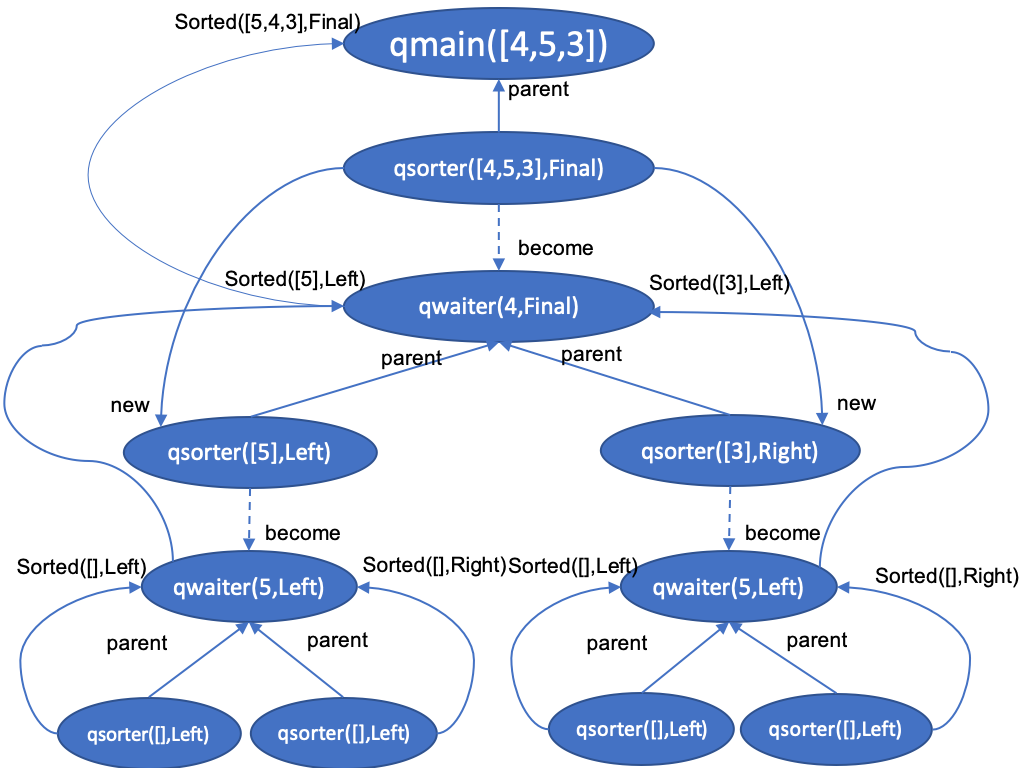
\includegraphics[width=\columnwidth]{qsort}
\caption{Example Quicksort}
\label{fig:example_quicksort}
\end{figure}

Figure \ref{fig:example_quicksort} shows a diagram representation of a simple quicksort in terms of the actors, their links and the messages that are sent. Note the dashed arrow showing \code{qsorter} actors becoming \code{qwaiter} actors.

\subsection{Termites}

\label{subsec:termites}

\begin{figure}
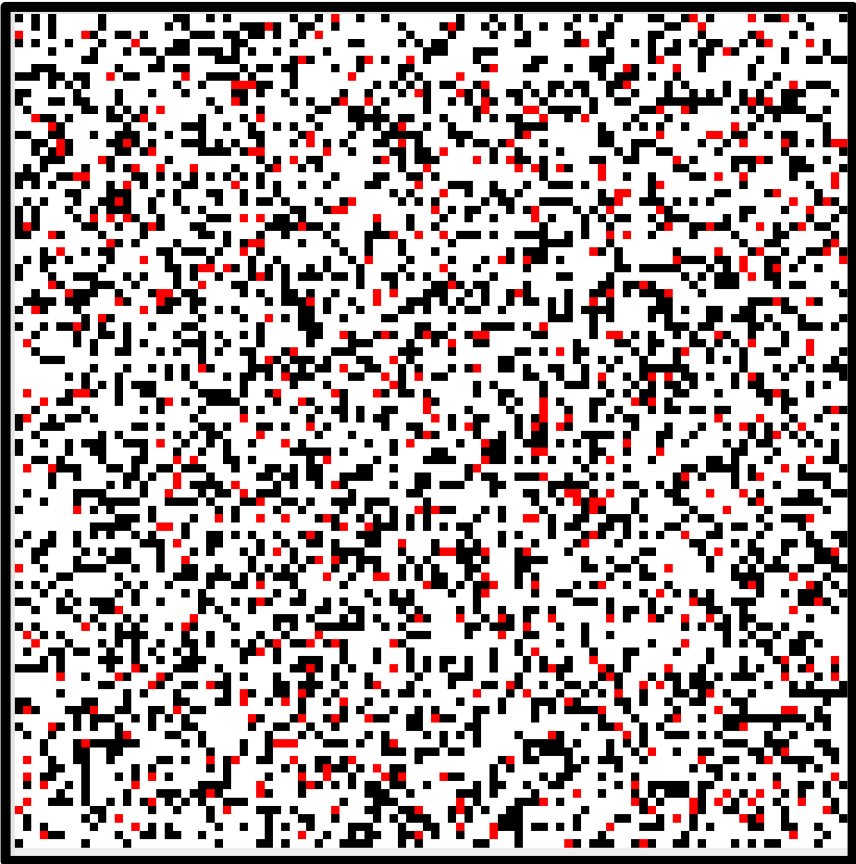
\includegraphics[width=0.4\columnwidth]{termites_before}
\hfill
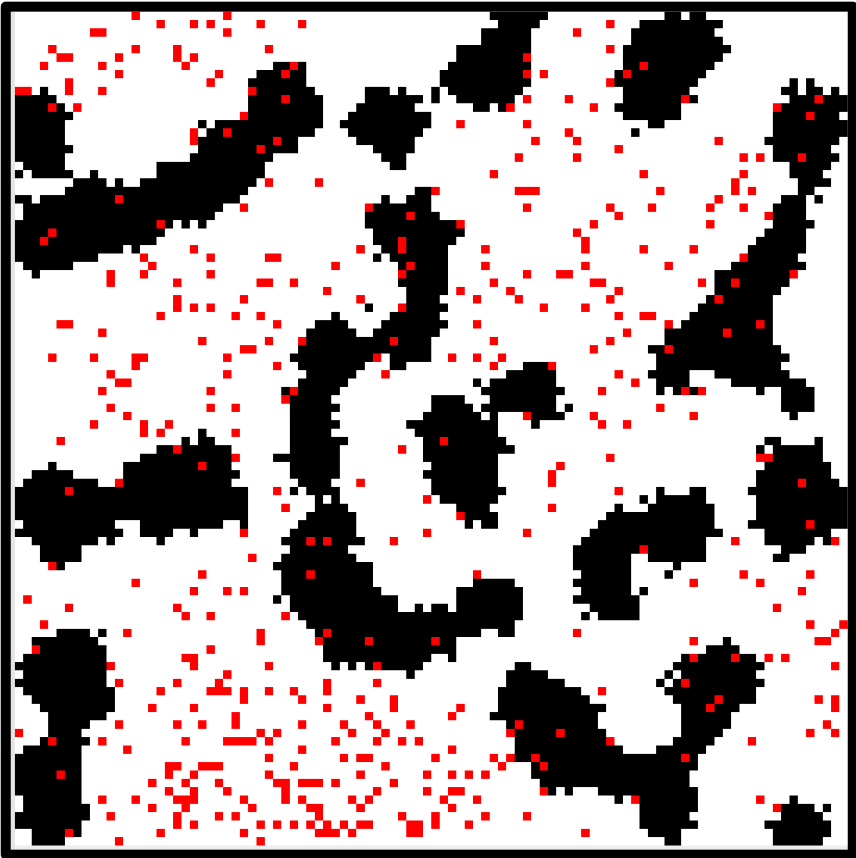
\includegraphics[width=0.41\columnwidth]{termites_after}
\caption{Termites Before and After}
\label{fig:termites}
\end{figure}

Actor based systems can be used to exhibit {\it emergent behaviour} where system-level behaviour can be observed as a result of many simple individual behaviours even though each individual behaviour has no knowledge of the whole. An example is {\it termites} shown in figure \ref{fig:termites} where a collection of twigs (black squares) and moved by a collection of termites (red squares) to form piles even though the individual termites do not have any knowledge of pile-formation.

The behaviour of a termite is simple: walk around at random until a twig is found that is not next to other twigs. The termite then picks up the lone-twig and walks at random until it finds another twig that is next to other twigs. The termite then drops the twig and then starts over again.


\begin{figure*}
%\hrule\textwidth1cm
\begin{multicols}{2}
\begin{ESL}
Act Main { Time(Int); }
Act Grid { SetColour(Int,Int,Str); TermiteAt(Int,Int,Int);}

size::Int          = 120;
limit::Int         = 40000;
numOfTermites::Int = 600;
twig::Str          = 'black';
background::Str    = 'white';
grid::Grid         = new 'esl.grid.Grid'[Grid](size,size,6); 

isLegal(x::Int,y::Int)::Bool = 
  (x >= 0 and x < size) and (y >= 0 and y < size);

Act Termite {  Search; Drop; FindSpace; GetAway(Int); }

act termite(id::Int,w::World)::Termite { 

  x::Int  = random(size);
  y::Int  = random(size);
  dx::Int = random(3) - 1;
  dy::Int = random(3) - 1;
  
  randomDir()::Void = {
    dx := random(3)-1;
    dy := random(3)-1;
  }
  move()::Void = {
    x := (x + dx); y := (y + dy);
    if x < 0 
    then { dx := 1; x := 0; move();
    } else if x > (size - 1)
    then { dx := -1; x := (size - 1); move();
    } else if y < 0 
    then { dy := 1; y := 0; move();
    } else if y > (size - 1)
    then { dy := 0 -1; y := (size - 1); move();
    } else grid <- TermiteAt(id,x,y);
  }
  moveRandom()::Void = {
    randomDir();
    move();
  }
  
  -> self <- Search;
  
  Search -> {
    moveRandom();
    w <- TryPickup(x,y,self);
  }
  Drop -> {
    moveRandom();
    w <- FindPile(x,y,self);
  }
  FindSpace -> {
    moveRandom();
    w <- TryDrop(x,y,self);
  }
  GetAway(0) -> {
    self <- Search;
  }
  GetAway(n::Int) -> {
    move();
    self <- GetAway(n-1);
  }
}


Act World {
  TryPickup(Int,Int,Termite);
  FindPile(Int,Int,Termite);
  TryDrop(Int,Int,Termite);
}

act world::World {
  locations::Array[Array[Str]] =
    let a::Array[Array[Str]] = new Array[Array[Str]](size);
    in {
      for x::Int in 0..size do {
        a[x] := new Array[Str](size);
        for y::Int in 0..size do {
          a[x][y] := if random(100) < 30 
                     then twig 
                     else background;
          grid <- SetColour(x,y,a[x][y]);
        }
      }
      edb.display[Grid]('Termites',grid); 
      a;
    }
  termites::[Termite] = 
    [ new termite(n,self) | n::Int <- 0..numOfTermites ];
  foundSingleton(x::Int,y::Int)::Bool = 
    locations[x][y] = twig and twigCount(x,y) < 5;
  foundPile(x::Int,y::Int)::Bool = 
    locations[x][y] = twig and twigCount(x,y) > 4; 
  isTwig(x::Int,y::Int)::Bool =  
    if isLegal(x,y) 
    then locations[x][y] = twig; 
    else false;
  twigCount(x::Int,y::Int)::Int = 
    sum([ if isTwig(x+dx,y+dy) then 1 else 0 | 
          dx <- [-1,0,1], 
          dy <- [-1,0,1], 
          ?(x<>0 or y<>0) ]);
      
  TryPickup(x::Int,y::Int,t::Termite) -> { 
    if foundSingleton(x,y)
    then {
      locations[x][y] := background;
      grid <- SetColour(x,y,background);
      t <- Drop;
    } else t <- Search;
  }
  FindPile(x::Int,y::Int,t::Termite) -> { 
    if foundPile(x,y)
    then t <- FindSpace;
    else t <- Drop;
  }
  TryDrop(x::Int,y::Int,t::Termite) -> {
    if locations[x][y] = background
    then {
      locations[x][y] := twig;
      grid <- SetColour(x,y,twig);
      t <- GetAway(20);
    } else t <- FindSpace;
  }
}

w::World = new world;

act main::Main {
  Time(n::Int) when n > limit -> stopAll();
  Time(n::Int) -> { } 
}
\end{ESL}
\end{multicols}
%\hrule\textwidth1cm\vspace{.5cm}
\caption{Termites}
\label{fig:esl_termites}
\end{figure*}

The implementation of termites in ESL is shown in figure \ref{fig:esl_termites}. The implementation shows a typical scenario in actor-based systems where there is a single world-state and many different actors that share the state. Each individual needs the state in order to determine its next move which involves an update to the world state. Given that all the actors are operating concurrently, this dependency on a single world state can cause problems if access and updates are not protected. Conventional programming languages provide {\it data locks} to deal with shared state. 

ESL provides locks, but often they are not required because actors operate in terms of asynchronous messages and queues. The diagram below shows how this works:
\begin{center}
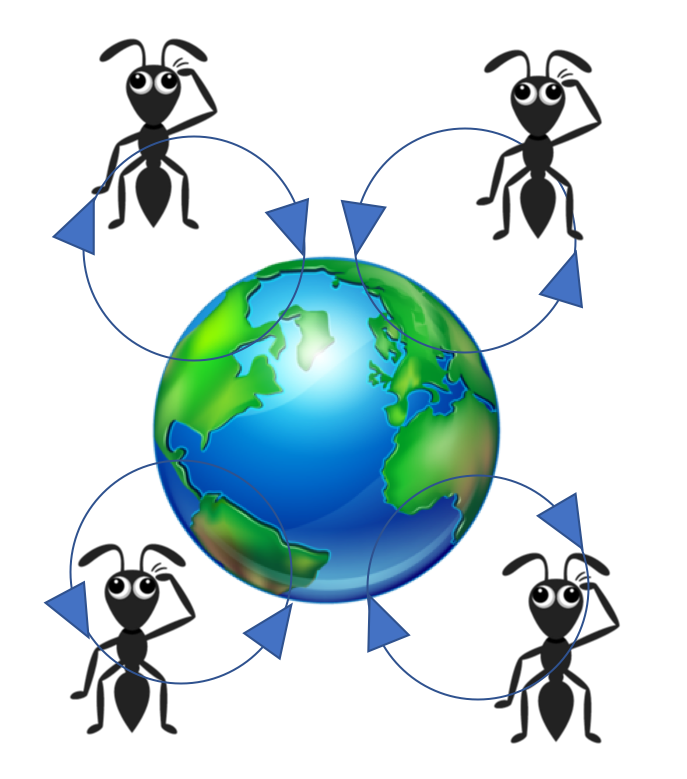
\includegraphics[width=0.5\columnwidth]{termites}
\end{center} 
The world at the centre of the figure represents the shared state. Four independent worker actors are shown, although any number can be involved. The shared state offers an interface that supports the operations required by the worker actors which, in turn, provide an interface that represents the different outcomes from performing the world operations.

From the perspective of a single worker, it looks like they get dedicated access to the shared world state because a message sent to the world is queued until the world becomes free. Each worker message must include the worker actor so that the shared state can reply to it. When a worker sends a message to the shared state the worker becomes idle and will be woken up by the reply from the shared state. When the shared state processes a worker message, the worker has exclusive access to the data, the data can be changed and then the message is sent back to the worker which is woken up.

\subsection{Dining Philosophers}

\label{sec:dining_philosophers}

Dining Philosophers is a standard scenario that is used to exemplify the issues of shared access to resources. Several concurrent processes (philosophers) are vying for shared resources (chopsticks) in order to eat. Each process needs exactly two resources to each and each resource is shared by exactly two processes. When a process acquires a pair of resources, it performs activity (eats) and then releases the resources. Access to resources is assumed to be fair. If a process acquires resources sequentially, then a situation can arise where all resources have acquired one resource and is awaiting on a resource that has been acquired by another process (starvation). In order to avoid starvation, the processes need to wait until they can individually acquire a pair of resources as an atomic action.

A situation where the philosophers are happily eating is shown below:
\begin{center}
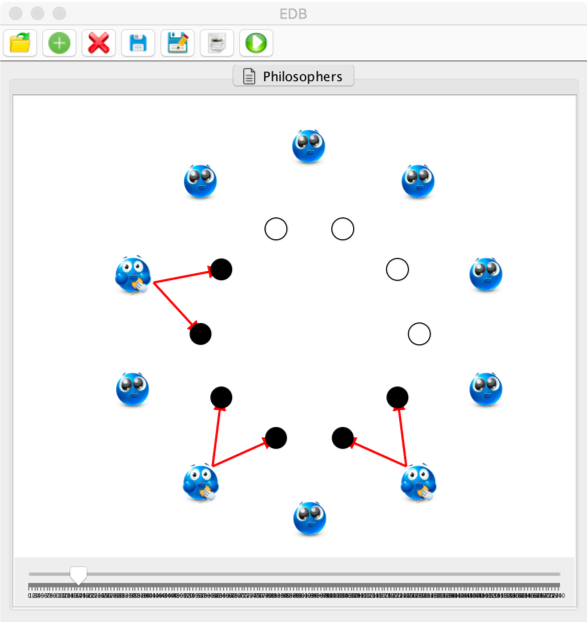
\includegraphics[width=0.49\columnwidth]{dining1}
\hfill
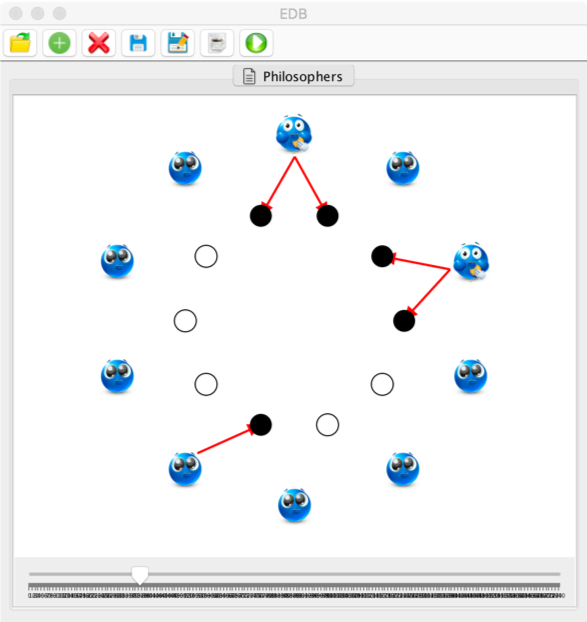
\includegraphics[width=0.49\columnwidth]{dining2}
\end{center}
In the case where chopsticks are grabbed one at a time, the situation rapidly deadlocks:

\begin{center}
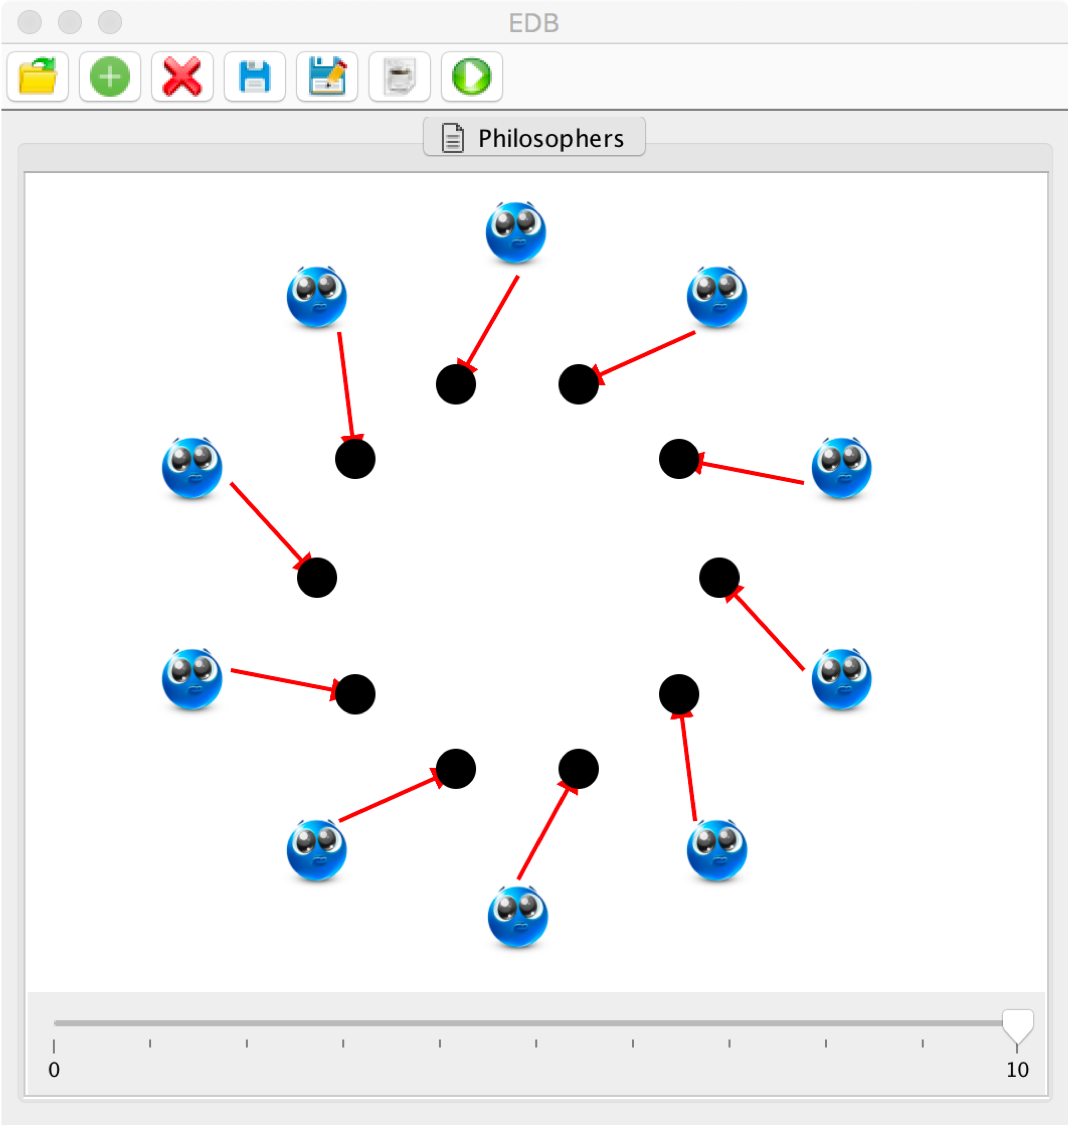
\includegraphics[width=0.49\columnwidth]{dining3}
\end{center}
The implementation of deadlock-free dining philosophers is shown below:
\begin{ESL}
numberOfPhilosophers::Int = 10;    
eatTime::Int              = 50;       
thinkTime::Int            = 50;   

Act Main { Time(Int); }
Act Chopstick { }  
Act Philosopher { Time(Int); }

eat()::Void   = wait(eatTime);
think()::Void = wait(thinkTime);

act philosopher(i::Int,
                left::Chopstick,
                right::Chopstick)::Philosopher {
  Time(n::Int) -> {
    think();
    grab(left,right) {
      eat();
    }  
  }
}

act chopstick::Chopstick {}

chopsticks::[Chopstick] = 
  [ new chopstick | i::Int <- 0..numberOfPhilosophers ];
chop(i::Int)::Chopstick = 
  nth[Chopstick](chopsticks,i%numberOfPhilosophers);

philosophers::[Philosopher] = 
  [ new philosopher(i,chop(i),chop(i+1))
  | i::Int <- 0..numberOfPhilosophers ]; 
\end{ESL}
Deadlock is avoided because the \code{grab} block acquires the locks on \code{left} and \code{right} at the same time. If the locks are not available then the \code{grab} block will wait until they are both free and acquire them simultaneously. Changing the definition of \code{philosopher} to the following leads to deadlock:
\begin{ESL}
act philosopher(i::Int,
                left::Chopstick,
                right::Chopstick)::Philosopher {
  Time(n::Int) -> {
    think();
    grab(left) {
      grab(right) {
        eat();
      }
    }  
  }
}
\end{ESL}

\subsection{Segregation}

\label{sec:segregation}

Thomas Schelling proposed an agent-based model of segregation in {\it Thomas C Schelling. Models of Segregation. American Economic Review, 59(2):488–493, 1969.} which demonstrates that relatively mild preferences for neighbours of a similar race can lead to high levels of segregation. The Schelling model shows how a completely random mix of two types of independent individuals:
\begin{center}
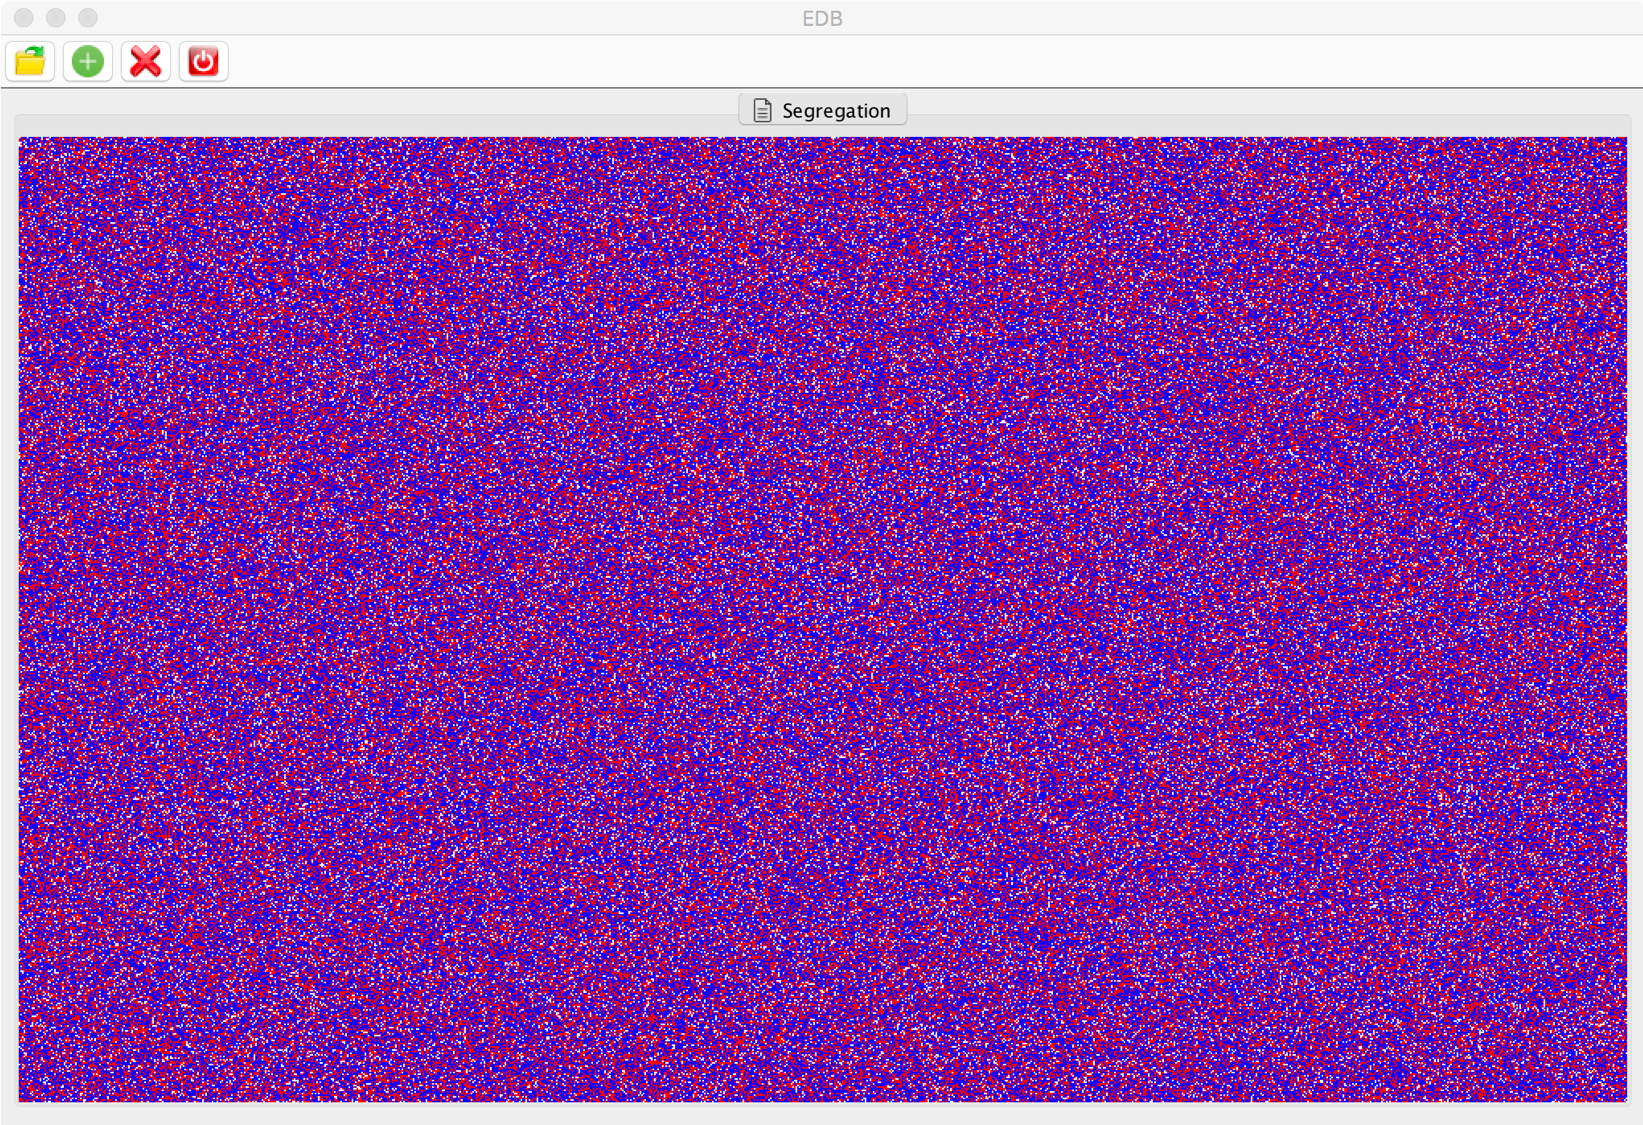
\includegraphics[width=0.8\columnwidth]{segregation1}
\end{center}
can lead to a structured outcome:
\begin{center}
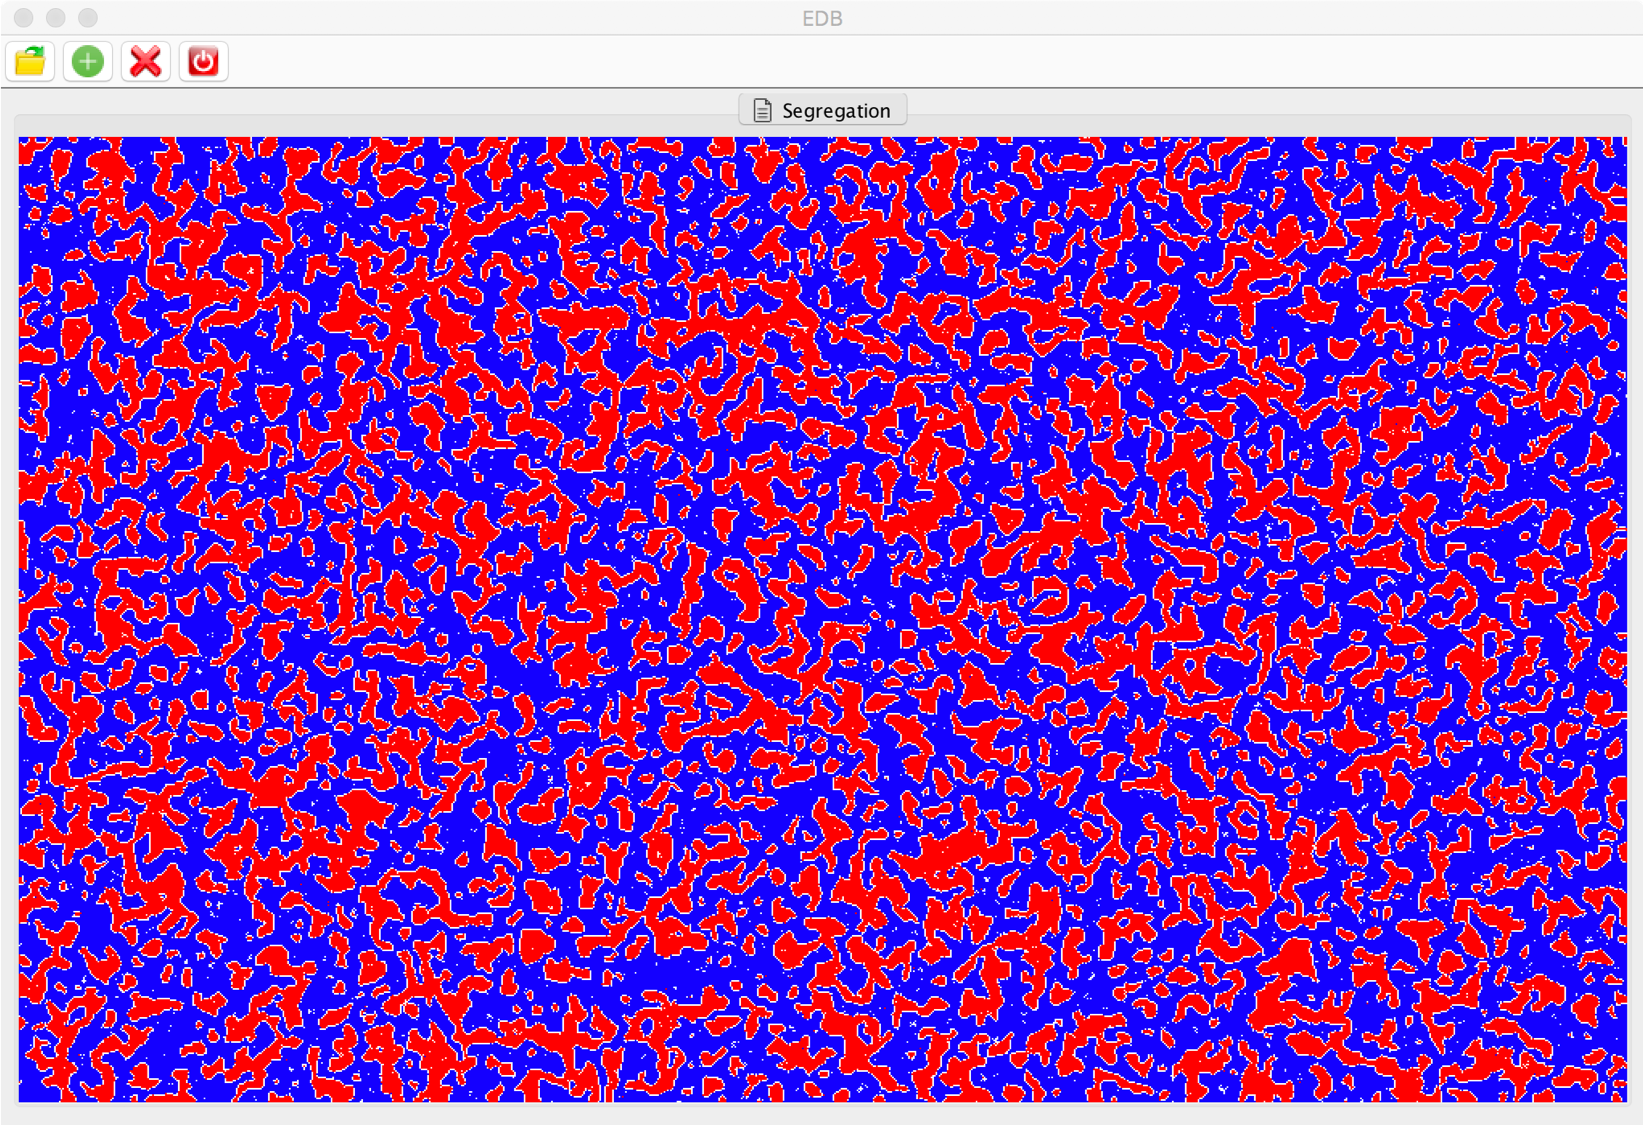
\includegraphics[width=0.8\columnwidth]{segregation2}
\end{center}
when none of the individuals would claim to have designed the outcome. This is another example of emergent behaviour, where relative simple individual behaviours can lead to a combined outcome that none of the individuals have planned for.

The data types used in the ESL implementation of segregation are shown below:
\begin{ESL}
type Main = Act { }

type Agent = Act { 
  export getX::()->Int; 
         getY::()->Int; 
         setX::(Int)->Void; 
         setY::(Int)->Void; 
}

type Grid = Act { 
  SetColour(Int,Int,Str); 
  Swap(Int,Int,Int,Int); 
} 

type Population = Act { 
  Move(Agent); 
}  

data Loc = Coord(Int,Int);
coordX(p::Loc)::Int = case p { Coord(x::Int,y::Int) -> x; }
coordY(p::Loc)::Int = case p { Coord(x::Int,y::Int) -> y; }
\end{ESL}
As we see below, an agent is just a passive structure with state. Each agent is singly threaded through the shared population state by a series of messages. A grid is a foreign actor implemented in Java which draws a colour at an \code{(x,y)} position and can swap the colours between two different locations. A population controls the grid.

An agent manages its state and initiates a sequence of messages to a population:
\begin{ESL}
act agent(x::Int,y::Int)::Agent {

  export getX,getY,setX,setY;

  getX()::Int = x;
  getY()::Int = y;
  setX(x0::Int)::Void = x := x0;
  setY(y0::Int)::Void = y := y0;

  -> population <- Move(self);
  
}
\end{ESL}
The following parameters and constants control the segregation application:
\begin{ESL}
diffLimit::Float = 25.00;  // % comfort limit.
width::Int       = 1000;   // with of population.
height::Int      = 600;    // height of population.
redpc::Int       = 40;     // % of population red.
emptypc::Int     = 10;     // % of population empty.
empty::Int       = 0;      // constant representing empty.
red::Int         = 1;      // constant representing red.
blue::Int        = 2;      // constant representing blue.
vLength::Int     = 0;      // number of vacancies.

opp(c::Int)::Int = if c = red then blue; else red;
colour(c::Int)::Str = 
  if c = red then 'red'; 
  else if c = empty then 'white'; 
  else 'blue';

legalx(x::Int)::Bool = (x >= 0) and (x < width);
legaly(y::Int)::Bool = (y >= 0) and (y < height);
\end{ESL}
The main work of the application is performed by the population actor:
\begin{ESL}
act pop::Population {

  createAgent(x::Int,y::Int)::Agent = {
    grid <- SetColour(x,y,colour(population[x][y]));
    new agent(x,y);
  }

  createVacancy(x::Int,y::Int)::Loc = {
    grid <- SetColour(x,y,colour(empty));
    Coord(x,y);
  }

  population::Array[Array[Int]] = 
    // Create the basic population...
    let a::Array[Array[Int]] = new Array[Array[Int]](width); 
    in {
      for w::Int in 0..width do {
        a[w] := new Array[Int](height);
        for h::Int in 0..height do {
          a[w][h] := 
            probably(100-emptypc)::Int { 
              probably(redpc)::Int 
                red; 
              else blue; 
            } else empty;
        }
      }
      a;
    }

  agents::Array[Array[Agent]] =
    // Create the agents...
    let a::Array[Array[Agent]] = 
          new Array[Array[Agent]](width);
    in {
      for x::Int in 0..width do {
        a[x] := new Array[Agent](height);
        for y::Int in 0..height do {
          a[x][y] := if population[x][y] <> empty 
                     then createAgent(x,y) 
                     else null[Agent];
        }
      }
      a;
    }

  createVacancies()::Array[Loc] =
    // create an array of vacancies for easy access...
    let vacancies::[Loc] = [ createVacancy(x,y) | 
                              x::Int <- 0..width, 
                              y::Int <- 0..height, 
                              ?(population[x][y]=empty) ];
    in {
      vLength := length[Loc](vacancies);
      let v::Array[Loc] = new Array[Loc](vLength);
      in {
        for i::Int in 0..vLength do {
          v[i] := nth[Loc](vacancies,i);
        }
        v;
      }
    }
  
  vacancies::Array[Loc] = createVacancies();
  
  popSet(x::Int,y::Int,c::Int)::Void =  population[x][y] := c;
  
  diffCellCount(x::Int,y::Int,c::Int)::Int =  length[Int]([ 1 | 
    dx <- [-1,0,1], 
    dy <- [-1,0,1], 
    ?not(dx=0 and dy=0),
    ?legalx(x+dx), 
    ?legaly(y+dy), 
    ?population[x+dx][y+dy] = c]);
    
  diffpc(x::Int,y::Int)::Float = 
    (intToFloat(diffCellCount(x,y,opp(population[x][y])))/8.0)*100.0;

  Move(a::Agent) -> { 
    let x::Int = a.getX(); y::Int = a.getY(); in
    if diffpc(x,y) > diffLimit 
    then 
      let i::Int = random(vLength); in
      let p::Loc = vacancies[i]; in
      let x0::Int = coordX(p); y0::Int = coordY(p);
      in { 
        vacancies[i] := Coord(x,y);
        popSet(x0,y0,population[x][y]);
        popSet(x,y,empty);
        grid <- Swap(x,y,x0,y0);
        a.setX(x0);
        a.setY(y0);
        self <- Move(a);
      } 
    else self <- Move(a);
  }
}
\end{ESL}
A \code{pop} actor receives a message \code{Move(a)}. Since the receiver is singly threaded, this provides \code{a} with exclusive access to the arrays \code{population} and \code{vacancies}. If each agent shared access to these resources, it is likely that movements could interleave and the state could become inconsistent. Once the move has occurred, the \code{pop} actor sends itself a \code{Move(a)} message which is queued with all other move requests. Since messages are delivered fairly, no agent is starved of movement.

\section{Polymorphism}

\label{sec:polymorphism}

When a function is defined, its type signature defines the types of its arguments and its return type. Consider the function \code{idInt}:
\begin{ESL}
idInt(x::Int)::Int = x;
\end{ESL}
which is similar to the function \code{idBool}:
\begin{ESL}
idBool(x::Bool)::Bool = x
\end{ESL} 
which is similar to many other functions such as \code{idFloat}, \code{idStr} and \code{idListOfInt}. In all cases the particular type of the argument is not relevant since the function always does the same thing: return the argument. It is important that the return type of the function is the same as the type of the argument. ESL allows a polymorphic function to be defined as follows:
\begin{ESL}
id[T](x::T)::T = x;
\end{ESL}
When such a definition is used, the particular types must be supplied:
\begin{ESL}
n::Int = id[Int](100);
b::Bool = id[Bool](true);
\end{ESL}
Multiple type arguments may be used. For example, the following is a function that applies a function \code{f} to all elements of a list in order to transform them from type \code{Source} to type \code{Target}:
\begin{ESL}
map[Source,Target](l::[Source],f::(Source)->Target)::[Target]=
  case l {
    [] -> [];
    h:t -> f(h) : map[Source,Target](t,f);
  }
\end{ESL}
Type functions provide abstractions over type definitions. The type function \code{ListOf} maps a type \code{T} to the type \code{[T]}:
\begin{ESL}
type ListOf[T] = [T];
\end{ESL}
Once defined, \code{ListOf[T]}, for some specific type expression \code{T} can be used as a type.

Data types can be defined parametrically. For example the following is a tree type for any type \code{T}:
\begin{ESL}
data Tree[T] =
  Branch(Tree[T],Tree[T]) 
| Leaf(T); 
\end{ESL}
Since the constructors \code{Branch} and \code{Leaf} are defined in the context of a type function, type arguments must be supplied when the constructors are used in patterns or to construct data values. For example:
\begin{ESL}
treeTrans[T1,T2](map::(T1) -> T2,t::Tree[T1])::Tree[T2] =
  case t {
    Branch[T1](l,r) -> Branch[T2](treeTrans[T1,T2](map,l),treeTrans[T1,T2](map,r));
    Leaf[T1](v)     -> Leaf[T2](map(v));
  }
\end{ESL}
and the two data values:
\begin{ESL}
t1::Tree[Int]  = 
  Branch[Int](Leaf[Int](100),Leaf[Int](200));
t2::Tree[Bool] = 
  treeTrans[Int,Bool](fun(i::Int)::Bool i > 100,t1);
\end{ESL}
The type mechanisms are hidden behind the language structures. If these are unpacked then the reason for the type arguments should be clear:
\begin{ESL}
type Tree = rec X. Fun[Y]
  union {
    Branch(X[Y],X[Y]),
    Leaf(Y)
  }
\end{ESL}
The constructor types in a union-type definition are viewed as function that inject into the union-type. Since the union-type is defined as a type function, the constructors must be supplied with a type whenever they are used.

\subsection{Map/Reduce}

\label{sec:mapreduce}

Map/reduce is an approach to processing large amounts of data that involves transforming the data and grouping with respect to keys. It is a pattern that is particularly suited to large amounts of concurrent processing because the mapping can occur independently and the grouping can be divided between different processing units. The approach has been used to help process internet data, such as counting the number of occurrences of text.

The diagram below shows how map/reduce works:
\begin{center}
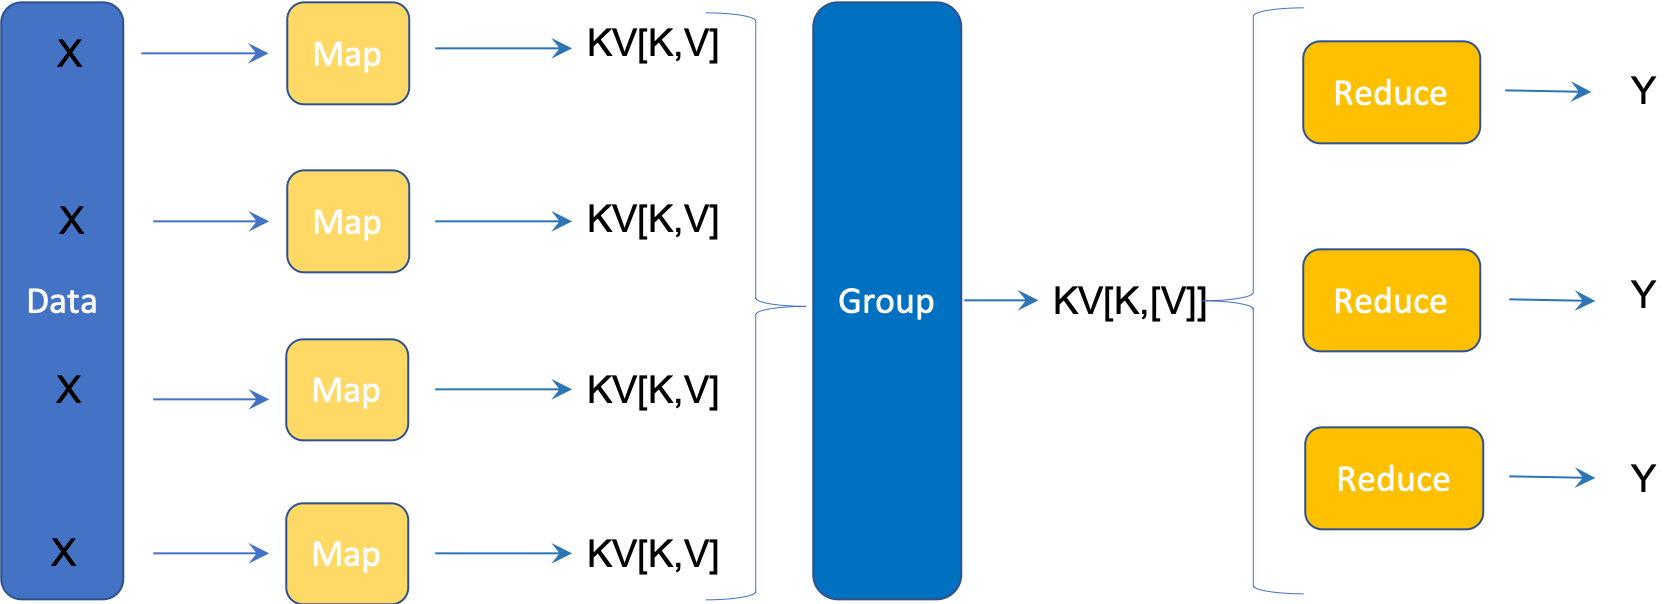
\includegraphics[width=\columnwidth]{map_reduce}
\end{center}
The data is of type \code{X} and is mapped to produce a collection of key-value pairs where the keys are of type \code{K} and the value of type \code{V}. Many different pairs may contain the same key; the pairs are grouped so that all the values associated with the same key are located together. Finally, each collection of values for the same key are reduced to produce a value of type \code{Y}. 

The map/reduce process is independent of the type of data \code{X}, the type of the keys \code{K} and the type of the target values \code{Y}. It is therefore a suitable candidate for polymorphism. The example will use a collection of words:
\begin{ESL}
import 'esl/strings.esl';

words::[Str] = splitBy(#\space,'Sed ut perspiciatis unde omnis iste natus error sit voluptatem accusantium doloremque laudantium, totam rem aperiam, eaque ipsa quae ab illo inventore veritatis et quasi architecto beatae vitae dicta sunt explicabo. Nemo enim ipsam voluptatem quia voluptas sit aspernatur aut odit aut fugit, sed quia consequuntur magni dolores eos qui ratione voluptatem sequi nesciunt. Neque porro quisquam est, qui dolorem ipsum quia dolor sit amet, consectetur, adipisci velit, sed quia non numquam eius modi tempora incidunt ut labore et dolore magnam aliquam quaerat voluptatem. Ut enim ad minima veniam, quis nostrum exercitationem ullam corporis suscipit laboriosam, nisi ut aliquid ex ea commodi consequatur? Quis autem vel eum iure reprehenderit qui in ea voluptate velit esse quam nihil molestiae consequatur, vel illum qui dolorem eum fugiat quo voluptas nulla pariatur?');
\end{ESL}
We will define a map/reduce implementation that uses polymorphic ESL actors to perform concurrent maps. The single implementation will be used in two ways: (1) to produce the number of words of each length; (2) to produce the number of occurrences of each word.
\begin{ESL}
Act Main {}

data KV[Key,Value] = Key(Key,Value); 
  
type Map[In]           = Act { Perform(In);              }
type Group[Key,Value]  = Act { Store(KV[Key,Value]);     } 
type Reduce[Key,Value] = Act { Process(KV[Key,[Value]]); }   
\end{ESL}
The data type \code{KV} is polymorphic with respect to the type of the key and the value. The type \code{Map} is a behaviour that it independent of the type of data items it processes via the \code{Perform} message. The type \code{Group} stores key-value pairs independent of they specific types, and the type \code{Reduce} processes key-value pairs after they have been grouped.

A map actor is created with the behaviour \code{mkMap}:
\begin{ESL}
act mkMap[In,Key,Value](f::(In)->KV[Key,Value],
                        g::Group[Key,Value])::Map[In]  {
  Perform(x::In) ->    
    g <- Store(f(x)); 
}
\end{ESL}
The \code{mkMap} function takes a mapping function \code{f} and a grouping actor \code{g}. When a map actor is sent a \code{Perform(x)} message it uses \code{f} to transform \code{x} to a key-value pair which is supplied to the grouping actor \code{g}.

A group actor has the following behaviour:
\begin{ESL}
act mkGroup[K,V](n::Int,reduce::Reduce[K,V])::Group[K,V] { 
  results :: [KV[K,[V]]] = [];
  add(x::KV[K,V],rs::[KV[K,[V]]])::[KV[K,[V]]] = 
    case x {                                                                          
      Key[K,V](i::K,v::V) -> 
        case rs {
          [] -> [Key[K,[V]](i,[v])];
          Key[K,[V]](j,vs):rs when i = j -> 
            Key[K,[V]](i,v:vs):rs;
          r:rs  -> r:add(x,rs);
        }
    }
  Store(x::KV[K,V]) when n = 1 -> { 
    results := add(x,results);
    for r::KV[K,[V]] in results do {
      reduce <- Process(r);
    }     
  }
  Store(x::KV[K,V]) -> { 
    results := add(x,results);
    n := n - 1;
  }
}
\end{ESL}
A group actor is supplied with the number of independent mappings \code{n} and a reducer actor \code{reduce}. The grouped results are maintained in the list \code{results}. Note that the type of \code{results} is \code{[KV[K,[V]]]}; the idea is that each key is associated with all the values supplied to the grouping agent. 

A grouping agent is supplied with key-value pairs in the message \code{Store(KV(k,v))}. If this not the last pair, then it is added to the results using \code{add} which ensures that all the values associated with the same key are grouped together. When the last key-value pair is received, the results are passed to the reducing actor.

Map/reduce is performed by the following function:
\begin{ESL}
mapReduce[In,Key,Value](l::[In],
                        f::(In)->KV[Key,Value], 
                        g::Group[Key,Value])::Void =      
  for x::In in l do {
    (new (mkMap[In,Key,Value])(f,g)) <- Perform(x);    
  }               
\end{ESL}

\subsubsection{All Words of a Given Length}

\begin{ESL}
act reduceWordLen::Reduce[Int,Str] {
  Process(r::KV[Int,[Str]]) ->
    case r {
      Key[Int,[Str]](i::Int,s::[Str]) -> 
        print[Str](i + ' ' + s);
    } 
}

strLen(s::Str)::KV[Int,Str] = 
  Key[Int,Str](length[Int](s.explode),s);

mapReduceWordLength()::Void =
  let r::Reduce[Int,Str] = new reduceWordLen; 
      n::Int = length[Str](words); in
  let g::Group[Int,Str] = new (mkGroup[Int,Str])(n,r); 
  in mapReduce[Str,Int,Str](words,strLen,g);
\end{ESL}

\subsubsection{Occurrences of a Word}

\begin{ESL}
act occurs::Reduce[Str,Int] {
  Process(r::KV[Str,[Int]]) ->
    case r {
      Key[Str,[Int]](s::Str,is::[Int]) ->
        print[Str](s + ' ocurrences = ' + length[Int](is));
    }
}

strOccurs(s::Str)::KV[Str,Int] = Key[Str,Int](s,1);

mapReduceOccurrences()::Void =
  let r::Reduce[Str,Int] = new occurs;
      n::Int = length[Str](words); in
  let g::Group[Str,Int] = new (mkGroup[Str,Int])(n,r);
  in mapReduce[Str,Str,Int](words,strOccurs,g);
\end{ESL}

\subsection{Cached Functions}

\label{sec:cache}

Single-argument functions without side effects can be cached so that the computation needed to produce the result is performed once and then added to a table. Subsequent applications of the function to the same argument will just look the value up in the table. Although the type of the argument and the return value differs between functions, the caching activity is the same in all cases. polymorphism can be used to abstract the type of the argument and return value:

\begin{ESL}
cache[Arg,Value](f::(Arg) -> Value)::(Arg) -> Value  =  
  let table::Hash[Arg,Value] = new Hash[Arg,Value];
  in {
    fun(a::Arg)::Value
      if table.hasKey(a)
      then table.get(a);
      else
        let v::Value = f(a);
        in {
          table.put(a,v);
          v;
        }
  }
\end{ESL}
Suppose we construct lists of the form \code{0..n} repeatedly for a range of values \code{n} where the same \code{n} may occur frequently. It is wasteful to construct the same list multiple times, especially if the value of \code{n} is high. It is much more efficient to use \code{cache}:
\begin{ESL}
getList::(Int) -> [Int] = cache[Int,[Int]](fun(n::Int) 0..n);
\end{ESL}

\section{Object Orientation}

\label{sec:object_orientation}

ESL supports subtypes and inheritance. Behaviour types can be defined as an extension of an existing behaviour type in which case all the message definitions and export declarations from the parent are included in the child. Whenever an identifier is declared to be of a particular behaviour type, any behaviour that conforms to an extension of the declared type can be supplied.

Behaviour definitions can extend a parent definition in which case the message handlers from the parent are all included in the child (in the same way that Java methods are inherited). Where the message signatures overlap, the child handlers will take precedence, but the parent definitions will be used where none of the child definition match. Parent local definitions are available in the child without qualification using the keyword \code{super}. This protects the integrity of the parent by making access to parent state and behaviour explicit.

To demonstrate ESL object-oriented features we will develop a Pacman game where inheritance allows position information to be abstracted into a behaviour that is then reused across players and ghosts. Sub-types are used to produce different types of ghosts and players.

The game consists of a maze containing 4 ghosts, some food and a Pacman. The Pacman moves around eating the food and the ghosts move around trying to catch the Pacman. The ghosts can only move horizontally and vertically whilst the Pacman can also move diagonally. No ghost or the Pacman can move through walls. At any given time, the ghosts are in one of two modes: \code{Scatter} and \code{Chase}. When in \code{Scatter} mode, the ghosts try to reach their home corner; each ghost has a different home:
\begin{center}
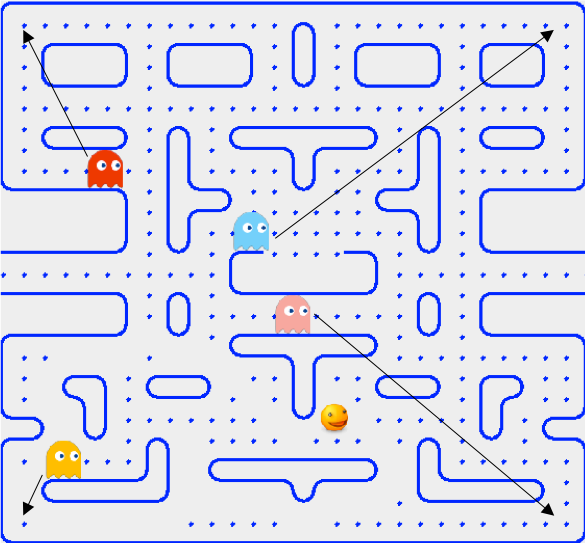
\includegraphics[width=0.8\columnwidth]{pac1}
\end{center}
When in \code{Case} mode, the ghosts head towards the Pacman and try to occupy the same location in which case the Pacman loses:
\begin{center}
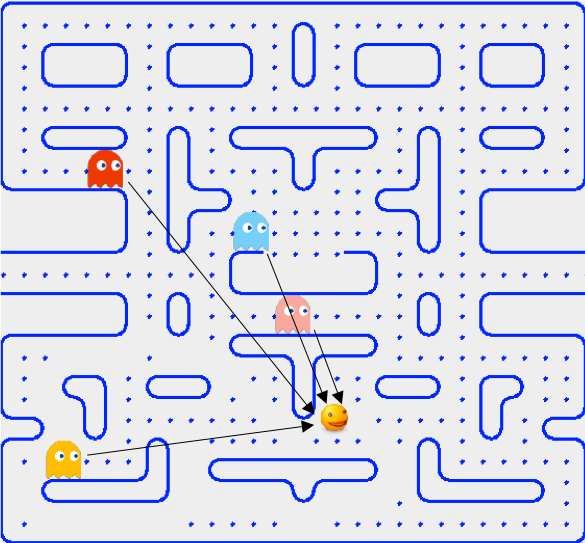
\includegraphics[width=0.8\columnwidth]{pac2}
\end{center}
The user interface is defined as an actor that is supplied with messages to update the Pacman maze:
\begin{ESL}
data GhostInfo = Point(Ghost,Int,Int,Int); // Point(g,type,x,y) 

data GhostState =
  Scatter
| Chase;

Act GUI {   
  export mouseX::Int; mouseY::Int; 
  State([GhostInfo],Array[Array[Int]]); 
  Player(Int,Int);
}
\end{ESL}
The Pacman maze is implemented as an actor with the behaviour type \code{Maze}. The maze provides the shared world state and ensures that actors move in turn each time the \code{Move} message is processed:
\begin{ESL}
Act Maze {
  export isWall::(Int,Int)->Bool;    
         atHome::(Int,Int)->Bool;  
         getPacman::() -> Pacman;  
         getGhosts::() -> [Ghost]; 
         legalPos::(Int,Int)->Bool;
         eat::(Int,Int)->Void;
  
  RegisterGhost(Ghost);   
  RegisterPacman(Pacman);  
  Move;        
}
\end{ESL}
All the actors in the maze will be sub-types of \code{Player} which provides basic features for location and starting to play:
\begin{ESL}
Act Player {
 export 
    getX::() -> Int;
    getY::() -> Int;
    setX::(Int) -> Void;
    setY::(Int) -> Void;
    getMaze::() -> Maze;
    moveTo::(Int,Int)->Void;
    move::()->Void;
    canMove::(Int,Int)->Bool;
    plan::(Int,
           (Plan,Plan)->Bool,
           (Plans)->Plan,
           (Plan)->Bool,
           (Plan)->[Loc],
           Plans) 
          -> Plan;
    moves::(Plan)->[Loc];
    deltaOK::(Int,Int)->Bool;
    initPlans::()->Plans;
    deltas::[Int];

  Start; 
}
\end{ESL}
The operation \code{move} is called to make a single-step move in the game. A player uses \code{plan} to plan out the move. The arguments of plan are as follows:
\begin{ESL}
plan(max,compare,goal,ok,moves,start)
\end{ESL}
where \code{max} determines the maximum length of the plan, \code{compare} is a predicate that compares plans such that \code{compare(p1,p2)} is true when \code{p1} is a better plan than \code{p2}, \code{goal} maps a collection of plans to a single plan that achieves a goal or returns \code{null}, \code{ok} returns true when a plan is legal, \code{moves} maps a plan to a sequence of locations that are legal next moves; \code{start} is a collection of starting plans (usually the current position of a player).

The \code{plan} operation is used to automatically generate next moves for players and is implemented differently for ghosts and the Pacman. Some of the player operations can be implemented and then reused across ghosts and players:
\begin{ESL}
ct player(x::Int,y::Int,maze::Maze)::Player {

  // A basic implementation of the player interface...
  
  export getX,getY,setX,setY,moveTo,getMaze,move,canMove,
         moves,plan,deltaOK,initPlans,deltas;

  getX()::Int = x;
  getY()::Int = y;
  setX(v::Int)::Void = x := v;
  setY(v::Int)::Void = y := v;
  moveTo(v1::Int,v2::Int)::Void = { x := v1; y := v2; }
  getMaze()::Maze = maze;
  move()::Void = throw[Void]('abstract operation move');
  canMove(x::Int,y::Int)::Bool = 
    maze.legalPos(x,y) or maze.atHome(x,y);
  deltas::[Int] =  [-1,0,1];
  deltaOK(dx::Int,dy::Int)::Bool = not(dx = 0 and dy = 0);
  initPlans()::Plans = [[Loc(self.getX(),self.getY())]];

  getBestPlan(better::(Plan,Plan)->Bool,plans::Plans)::Plan =
    select1[Plan](plans,null[Plan],fun(p1::Plan)::Bool
      not(exists[Plan](fun(p2::Plan)::Bool
        p1 <> p2 and better(p2,p1),plans)));
        
  plan(max::Int, better::(Plan,Plan)->Bool,
       goal::(Plans)->Plan,pred::(Plan)->Bool,
       moves::(Plan)->[Loc],plans::Plans)::Plan = 
    if plans = []
    then null[Plan];
    else if max < 0
    then getBestPlan(better,plans); 
    else 
      let p::Plan = goal(plans);
          plans::Plans = 
            [p | p <- addMoves(plans,moves), ?pred(p)];
      in if p = null[Plan]
         then plan(max-1,better,goal,pred,moves,plans);
         else p;

  hasMove(m::Loc)::(Plan)->Bool = 
    fun(p::Plan)::Bool member[Loc](m,p);

  addMoves(plans::Plans,moves::(Plan)->[Loc])::Plans =
    [ m:p | p <- plans, 
            m <- moves(p), 
            ?(not(exists[Plan](hasMove(m),plans))) ];

  moves::(Plan) -> [Loc] = 
    cache[Plan,Loc,[Loc]](head[Loc],fun(p::Plan)::[Loc] 
      case head[Loc](p) {
        Loc(x::Int,y::Int) -> 
          [ Loc(x+dx,y+dy) | 
              dx <- deltas, 
              dy <- deltas, 
              ?(self.deltaOK(dx,dy)), 
              ?(canMove(x+dx,y+dy)) ];
      });
     
  Start -> throw[Void]('abstract message Start');
}
\end{ESL}
In \code{player} the implementation of \code{plan} uses the supplied arguments to map a collection of plans to a single best plan. A plan is a sequence of locations, in reverse order, that are a legal sequence of moves from some starting position. The operation \code{addMoves} is used by \code{plan} to add a new move to the end of each plan. A check is made in \code{addMoves} to ensure that no plan contains a cycle.


*****************

In Pacman there are four types of ghost. Each type has a different behaviour which will be implemented as different sub-behaviours of a common parent behaviour \code{ghost}. The maze is drawn by a Swing-based Java application that will draw the ghosts in different colours, supplied to the Java as integer codes that are the value of \code{ghostType}:
\begin{ESL}
Act Ghost extends Player { export ghostType::Int; }
\end{ESL}
We create an empty behaviour type as placeholder in the hierarchy for players:
\begin{ESL}
Act Pacman extends Player { }
\end{ESL}

\begin{figure*}
\begin{ESL}
act ghost(x::Int,y::Int,homeX::Int,homeY::Int,gType::Int,m::Maze)::Ghost extends player(x,y,m) {
  export ghostType, move;

  ghostType::Int     = gType;        // The type of the ghost.
  state::GhostState  = Chase;        // Current state, used for planning.
  changeMode::Int    = 15;           // Change the state after this number of moves.
  modeCount::Int     = changeMode;   // Current countdown to change state.
  maxPlanLength::Int = 8;            // Select the best plan after this number of plan steps.

  move()::Void = 
    letrec 
      selectMin(r::(Plan,Plan)->Bool,plans::[Plan])::Plan = 
        select1[Plan](plans,null[Plan],fun(p1::Plan)::Bool 
          forall[Plan](fun(p2::Plan)::Bool if p1=p2 then true else r(p1,p2),plans));
      planDistance(p::Plan,x::Int,y::Int)::Float = case head[Loc](p) { Loc(x0,y0) -> distance(x,y,x0,y0); }
      plan(goalX::Int,goalY::Int,plans::Plans)::Plan = 
        // Create a plan that takes the ghost nearest to the goal position...
        if length[Loc](head[Plan](plans)) > maxPlanLength
        then 
          selectMin(fun(p1::Plan,p2::Plan)::Bool planDistance(p1,goalX,goalY) <= planDistance(p2,goalX,goalY),plans);
        else 
          let p::Plan = select1[Plan](plans,null[Plan],fun(p::Plan)::Bool head[Loc](p) = Loc(goalX,goalY));
          in if p = null[Plan]
             then plan(goalX,goalY,[ m:p | 
               p <- plans,m <- moves(p),?(not(exists[Plan](fun(p::Plan)::Bool member[Loc](m,p),plans))) ]);
             else p;
      getMove(goalX::Int,goalY::Int)::Loc = 
        // Get a move towards the goal...
        case plan(goalX,goalY,[[Loc(self.getX(),self.getY())]]) {
          [Loc(x,y)] -> Loc(x,y);           // Nothing available, no move.
          p -> last[Loc](butlast[Loc](p));  // Plan is in reverse and contains current location.
        }
      moves::(Plan) -> [Loc] = cache[Plan,Loc,[Loc]](head[Loc],fun(p::Plan)::[Loc] 
        // Get the available moves based on the location at the head of the supplied plan...
        case head[Loc](p) {
          Loc(x::Int,y::Int) -> 
            [ Loc(x+dx,y+dy) | dx <- [-1,0,1], dy <- [-1,0,1], ?(not(x=0 and y=0)), ?(self.canMove(x+dx,y+dy)) ];
        });
    in {
      case state {
        Scatter when modeCount > 0 ->  // Scattering heads towards the home location...
          case getMove(homeX,homeY) {
            Loc(x::Int,y::Int) -> {
              self.moveTo(x,y);
              modeCount := modeCount - 1;
            }
          }
        Scatter -> { // Switch mode to chasing the pacman...
          state := Chase;
          modeCount := changeMode;
        }
        Chase when modeCount > 0 ->  // Chasing heads towards the pacman...
          case getMove(m.getPacman().getX(),m.getPacman().getY()) {
            Loc(x::Int,y::Int) -> {
              self.moveTo(x,y);
              modeCount := modeCount - 1;
            }
         }
        Chase -> { // Switch mode to heading back home...
          state := Scatter;
          modeCount := changeMode;
        }
      }
    }

  Start -> 
    m <- RegisterGhost(self);
}
\end{ESL}
\caption{Abstract Ghost Behaviour}
\label{fig:abstract_ghost}
\end{figure*}


Figure \ref{fig:abstract_ghost} defines an abstract ghost behaviour that inherits the behaviour \code{player}. A ghost exists in one of two states: \code{Chase} and \code{Scatter} which controls whether it is trying to catch the Pacman or trying to reach its home position. It achieves this by creating a plan using the local function \code{plan}. A plan is created by extending a collection of current plans with all the possible legal moves calculated by the function \code{moves}. The length of the plan is controlled by \code{maxPlanLength}; when this is reached, the best plan is selected amongst all the available plans. The best plan is that which minimises the distance to the goal location.

Having defined an abstract ghost behaviour we can extend it to produce four different concrete ghost behaviours. In the real game, the ghosts differ by strategy to catch the Pacman, however we will limit the differences to the home locations:
\begin{ESL}
act ghost1(x::Int,y::Int,m::Maze)::Ghost 
  extends ghost(x,y,1,1,0,m) { }
act ghost2(x::Int,y::Int,m::Maze)::Ghost 
  extends ghost(x,y,1,maxHeight-2,1,m) { }
act ghost3(x::Int,y::Int,m::Maze)::Ghost 
  extends ghost(x,y,maxWidth-2,1,2,m) { }
act ghost4(x::Int,y::Int,m::Maze)::Ghost 
  extends ghost(x,y,maxWidth-2,maxHeight-2,3,m) { }
\end{ESL}
An abstract Pacman is a player that registers itself with the maze:
\begin{ESL}
act pacman(x::Int,y::Int,m::Maze)::Pacman 

  extends player(x,y,m) {
  
  Start -> 
    m <- RegisterPacman(self);
}
\end{ESL}
There will be two different concrete Pacman behaviours. The first allows a human player to control the Pacman using the mouse. This will be achieved by querying the current mouse position:
\begin{ESL}
act playerPacman(x::Int,y::Int,m::Maze)::Pacman  

  extends pacman(x,y,m) {
  
  export move;
  
  move()::Void = {
    let mouseX::Int = gui.mouseX;
        mouseY::Int = gui.mouseY; 
        x::Int = self.getX(); y::Int = self.getY(); in
    let dx::Int = mouseX - x;
        dy::Int = mouseY - x; in
    let mx::Int =if dx>0 then 1;else if dx<0 then -1;else 0;
        my::Int =if dy>0 then 1;else if dy<0 then -1;else 0;
    in {
      if (mx <> 0) and m.legalPos((x+mx)%maxWidth,y)
      then self.setX((x+mx)%maxWidth);
      else 
        if (my <> 0) and 
           m.legalPos(x,y+my)
        then self.setY(y+my);
        else 
          if m.legalPos((x+mx)%maxWidth,y+my) 
          then self.moveTo((x+mx)%maxWidth,y+my);
          else  
            if x + mx = 0 and m.legalPos(0,y)
            then self.setX(maxWidth -1);
            else {}
      gui <- Player(x,y);
      m.eat(x,y);
    }
  } 
}
\end{ESL}
\begin{figure*}
\begin{ESL}
act autoPacman(x::Int,y::Int,m::Maze)::Pacman extends pacman(x,y,m) { export move;
  plan::Plan             = [];         // A sequence of locations in reverse order.
  fleeing::Bool          = false;      // Is the pacman in danger of being eaten?
  
  moves::(Plan) -> [Loc] = cache[Plan,Loc,[Loc]](head[Loc],fun(p::Plan)::[Loc] 
    case head[Loc](p) {
      Loc(x::Int,y::Int) ->
        [ Loc(if x+dx = 0 then maxWidth-1 else x+dx,y+dy) |  dx::Int <- [1,0,-1], dy::Int <- [1,0,-1], 
            ?(not(dx=0 and dy=0)), 
            ?(self.canMove(x+dx,y+dy)) ];
    });

  ghostDistance(l::Loc)::Float = min(1000.0,[ distance(locX(l),locY(l),g.getX(),g.getY()) | g::Ghost <- m.getGhosts() ]);

  nextMove(p::Plan)::Loc = case p {  p1 + [l] + p2 when length[Loc](p2) = 1 -> l; }
      
  move()::Void =
    let d::Float = ghostDistance(Loc(self.getX(),self.getY()));
    in if d < 5.0 and not(fleeing) then { flee(7); fleeing := true; doPlan(); } 
       else if d > 5.0 and fleeing then { eat(9); fleeing := false; doPlan(); } 
       else doPlan();

  ghostMoves::(Loc) -> [Loc] = cache[Loc,Loc,[Loc]](id[Loc],fun(l::Loc)::[Loc]
    case l { Loc(x::Int,y::Int) ->
      [ Loc(x+dx,y+dy) | dx <- [1,0,-1], dy <- [1,0,-1], ?(dx=0 or dy=0), ?(not(dx=0 and dy=0)), ?(self.canMove(x+dx,y+dy)) ];
    });

  getDangerZones(moves::Int)::[[Loc]] = 
    letrec ghostLocs::[Loc] = [ Loc(g.getX(),g.getY()) | g::Ghost <- m.getGhosts() ];
           zones(zone::[Loc],i::Int,max::Int)::[[Loc]] =
             if i >= max then []; else let z::[Loc] = [ m  | l::Loc <- zone, m::Loc <- ghostMoves(l) ]; in z:zones(z,i+1,max);
    in zones(ghostLocs,0,moves);

  eat(n::Int)::Void =
    letrec dangerZones::[[Loc]] = getDangerZones(n+1);
           eatPlans(plans::Plans,i::Int,max::Int)::Plans =
             if i >= max then plans;
             else eatPlans([ l:p |  p <- plans, l <- moves(p),
               ?(not(exists[[Loc]](fun(zone::[Loc])::Bool member[Loc](l,zone),take[[Loc]](dangerZones,i+1)))),
               ?(not(exists[Plan](fun(p::Plan)::Bool member[Loc](l,p),plans)))
             ],i+1,max);
       foodCount(plan::Plan)::Int = let count::Int=0; in { for l in plan do count := count + food[locY(l)][locX(l)]; count;}
       moreFood(plan1::Plan,plan2::Plan)::Bool = foodCount(plan1) > foodCount(plan2);
       mostFood(plans::Plans)::Plan = max[Plan](plans,moreFood);
    in case mostFood(eatPlans([[Loc(self.getX(),self.getY())]],0,n)) {
         p when p = null[Plan] -> { print[Str]('Yikes - no plan!'); plan := []; }
         p -> plan := butlast[Loc](p);
       }

  flee(n::Int)::Void = 
    letrec dangerZones::[[Loc]] = getDangerZones(n+1); 
           fleePlans(plans::Plans,i::Int,max::Int)::Plans =
             if i >= max  then plans;
             else fleePlans([ l:p | p::Plan <- plans, l::Loc <- moves(p),
               ?(not(exists[[Loc]](fun(zone::[Loc])::Bool member[Loc](l,zone),take[[Loc]](dangerZones,i+1)))),
               ?(not(exists[Plan](fun(p::Plan)::Bool member[Loc](l,p),plans)))
             ],i+1,max);
    in case fleePlans([[Loc(self.getX(),self.getY())]],0,n) {
         [] -> { print[Str]('Yikes - no plan!'); plan := []; }
         p:ps -> plan := butlast[Loc](p);
       }

  doPlan()::Void =
    if plan = [] then replan(); else case plan {
      p1 + [l] -> { plan := p1; case l { Loc(x,y) -> { self.moveTo(x,y);  gui <- Player(self.getX(),self.getY()); } }
    }

  replan()::Void = if fleeing then flee(7); else eat(9);
}
\end{ESL}
\caption{Automatic Pacman}
\label{fig:auto_pacman}
\end{figure*}


An alternative implementation of the player provides a machine implemented behaviour. Like ghosts, the automatic movement is defined by a simple planner that tries to maximise the amount of food that is eaten whilst avoiding ghosts.

















The following variables control the game:
\begin{ESL}
cellWidth::Int         = 20;    // Used to convert the (mouseX,mouseY) positions.
cellHeight::Int        = 20;    // Used to convert the (mouseX,mouseY) positions.
maxWidth::Int          = 29;    // Max number of horizontal locations in the maze.
maxHeight::Int         = 27;    // Max number of vertical locations in the maze.
delay::Int             = 100;   // Used to slow down the game.
cellEmpty::Int         = 0;     // Code for an empty cell.
legalCell::Int         = 2;     // No occupation above this code.
homeCell::Int          = 3;     // Code for ghost home.
hWall::Int             = 4;     // Code for a horizontal wall.
vWall::Int             = 5;     // Code for a vertical wall.
topLeftCorner::Int     = 6;     // Code for a top-left corner.
topRightCorner::Int    = 7;     // Code for a top-right corner.
bottomLeftCorner::Int  = 8;     // Code for a bottom-left corner.
bottomRightCorner::Int = 9;     // Code for a bottom-right corner.
timeLimit::Int         = 70000; // How long to run the game.
\end{ESL}



\section{EDB}

\label{sec:edb}

EDB is an editor-based development environment for ESL that integrates syntax checking, type checking, compilation, application execution and run-time debugging. EDB relies on access to a Java compiler as 
provided by:\\
\code{
javax.tools.ToolProvider.getSystemJavaCompiler()}

At startup, EDB is supplied with the following run-time Java arguments in order:
\begin{enumerate}
\item A path to the directory that contains the ESL source code. From the root installation directory, this will be \code{esl}.
\item A path to a directory containing EDB data that is saved between executions. This includes information about the current state of EDB when it is shut down so that it can be recreated.
\end{enumerate}
EDB consists of a collection of tabs. Each tab has a particular type:
\begin{description}
\item[HTML] Contains HTML that has been generated by an ESL application or from a file. The HTML is displayed using a browser implemented by JxBrowser\footnote{\url{https://www.teamdev.com/jxbrowser}}. Handlers can be registered with EDB that process hyperlinks when they are clicked.
\item[ESL] Contains the contents of an ESL file that can be edited within EDB, written to the file system, compiled to produce Java and then run. An ESL tab provides syntax checking and type checking for the ESL language.
\item[Java] EDB is not intended to provide extensive support for Java development, however it provides limited support for editing, pretty-printing and compilation of Java source code to support the debugging and modification of Java that is produced when ESL is compiled.
\item[TabbedActor] Java based applications that use Swing libraries can be integrated into EDB by defining a class that implements the \code{edb.editor.TabbedActor} interface and that extends a Java Swing container. \end{description}

\subsection{EDB Interface}

\label{sec:edb_interface}

\begin{figure*}[t]
\centering
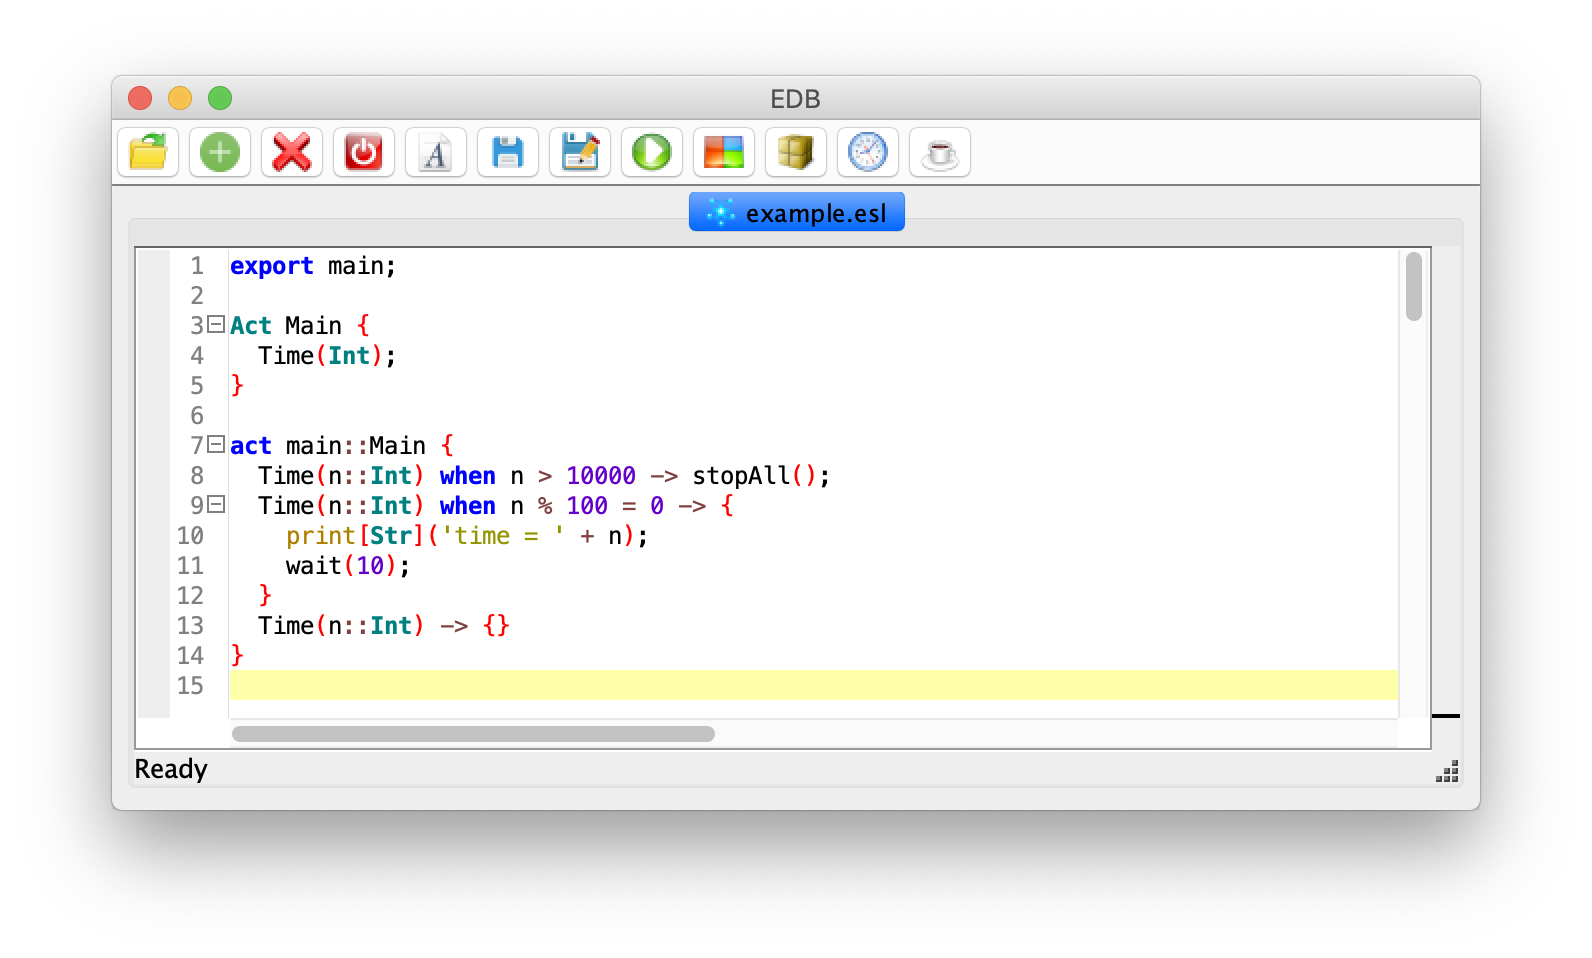
\includegraphics[width=\textwidth]{edb}
\caption{EDB Showing an ESL Tab}
\label{fig:edb}
\end{figure*}

The EDB interface is shown in figure \ref{fig:edb} with a single ESL tab. The text is highlighted according to ESL syntax rules which are checked dynamically as the text is modified. Errors are shown in two ways: (1) by underlining the text containing the error in red; (2) as a red marker in the margin. Hovering over either of these  with the mouse will describe the error. 

The toolbar buttons provide access to EDB functionality. For an ESL tab the following functionality is supported:

\noindent
\begin{tabular}{|c|c|p{2in}|}
\hline
{\bf button}&{\bf key}&{\bf description}\\\hline

\includegraphics[width=0.5cm]{../../icons/load.png}& & Load file into EDB.
\\\hline

\includegraphics[width=0.5cm]{../../icons/new_file}& & Create new file.
\\\hline

\includegraphics[width=0.5cm]{../../icons/delete}& & Delete file.
\\\hline

\includegraphics[width=0.5cm]{../../icons/stop}& & Stop a running application.
\\\hline

\includegraphics[width=0.5cm]{../../icons/font}& & Change font.
\\\hline

\includegraphics[width=0.5cm]{../../icons/save}& Meta-S & Save file.
\\\hline

\includegraphics[width=0.5cm]{../../icons/save_as}& & Save file as.
\\\hline

\includegraphics[width=0.5cm]{../../icons/clock}& Meta-T & Touch file and imports.
\\\hline

\includegraphics[width=0.5cm]{../../icons/compile}& Meta-K & Compile ESL to Java.
\\\hline
\end{tabular}

Pressing command and clicking on an identifier in an ESL editor will jump to its definition. The background menu provides access to all definitions via their name. All the defined names in an ESL file can be copied to the clipboard via the background menu; this is very useful in order to export the names in a file via the \code{export} clause at the start of the file, which can be created via copy and paste.

A Java tab provides a subset of the ESL functionality in addition to:

\noindent
\begin{tabular}{|c|c|p{2in}|}
\hline
{\bf button}&{\bf key}&{\bf description}\\\hline
\\\hline

\includegraphics[width=0.5cm]{../../icons/java_file}& Meta-J & Pretty print the Java source.
\\\hline

\includegraphics[width=0.5cm]{../../icons/run}& Meta-R & Compile and run file.
\\\hline
\end{tabular}

Both types of editor support a background menu that offers functionality for search, find and replace, copy text as a bitmap to the clipboard, and zoom. 

\subsection{EDB Actor}

\label{sec:edb_actor}

EDB can be referenced within a running ESL application using the variable \code{edb} whose type is defined in the module \code{esl/displays.esl}:
\begin{ESL}
Act EDB {
  export 
    math::Math;
    message::Forall[T] (T)->T; 
    display::Forall[T] (Str,T)->Void; 
    button::(Str,Str,Str,Str,()->Void)->Void; 
  Show(Str,Display);
  Filmstrip(Str,[Display]);
  AddBrowserListener(BrowserListener);
  Edit(EditType);
}

type Math = {
  circlePos::(Int,Int,Int,Int) -> Point
};

Act BrowserListener {
  BrowserEvent(Str);
}

data EditType =
  ESLSource(Str,Str)
| JavaSource(Str,Str,Str)
| RawText(Str);
\end{ESL}
The EDB object can be used to display graphics (as described below), register hyperlink event listeners, and to edit source code by creating an EDB tab.

\subsection{EDB Displays}

\label{sec:displays}

EDB supports a data type \code{Display} that can be used to create a variety of graphical displays. Sending the message:
\begin{ESL}
edb <- Show(label,display);
\end{ESL}
creates (or replaces) an EDB tab with the supplied label and the graphical display. The display type \code{Display} is defined in appendix \ref{sec:display_definitions}.

\subsection{Tables}

\label{sec:tables}

EDB can display HTML tables, for example the following table:
\begin{center}
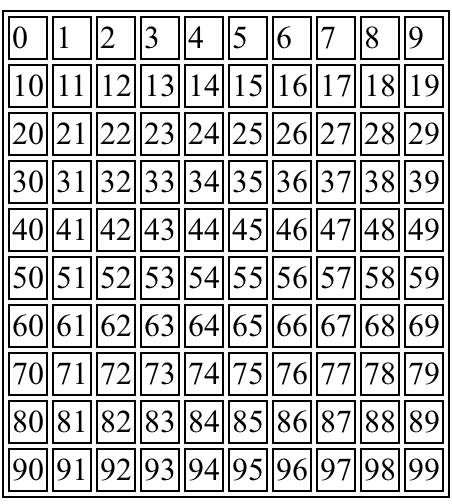
\includegraphics[width=0.6\columnwidth]{table}
\end{center}
is produced by:
\begin{ESL}
props::Props = [Prop('style','border: 1px solid black;')];

table::Display = 
  Table(props,
    [ Row([],
       [ Data(props,HTML('' + j)) 
       | j <- (i*10)..((i*10)+10) 
       ]) 
    | i <- 0..10 
    ]);
edb <- Show('mytable',table);
\end{ESL}
Since tables are HTML, it is possible to include links. The links are processed using browser events:
\begin{ESL}
props::Props = [Prop('style','border: 1px solid black;')];

table::Display = 
  Table(props,
    [ Row([],
       [ Data(props,
           HTML('<a href="edb:' + j + '">' + j + '</a>')) 
       | j <- (i*10)..(i*10)+10 
       ]) 
    | i <- 0..10
    ]);
  
act tableListener::BrowserListener {
  BrowserEvent('50') -> stopAll();
  BrowserEvent(s::Str) -> print[Str]('you pressed: ' + s);
}

edb <- AddBrowserListener(new tableListener);
edb <- Show('mytable',table);
\end{ESL}
Produces the following table:
\begin{center}
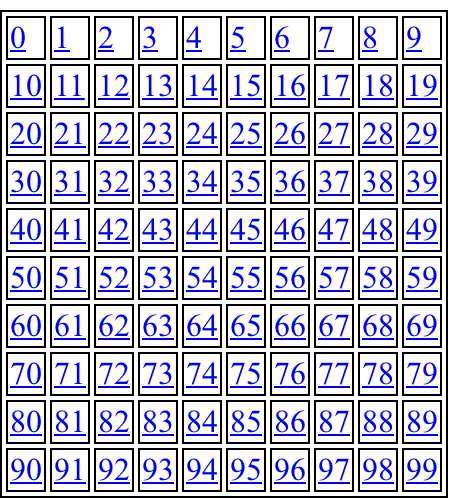
\includegraphics[width=0.6\columnwidth]{links}
\end{center}
Clicking on any of the links (except \code{50}) prints the number. Clicking on \code{50} stops the application. Subsequent clicks do nothing.

%%% Shop

\subsection{Pie Charts}

\label{sec:pie}

Pie charts can show results. The values associated with each slice are shown as proportions of the pie:
\begin{ESL}
pie::Display = Pie([],'Annual Car Sales',400,400,[
  Slice([],'VW',20),
  Slice([],'Vauxhall',10),
  Slice([],'Audi',20),
  Slice([],'Ford',10),
  Slice([],'Bentley',3),
  Slice([],'Volvo',40)]);
  
edb <- Show('mypie',pie);
\end{ESL}
which produces:
\begin{center}
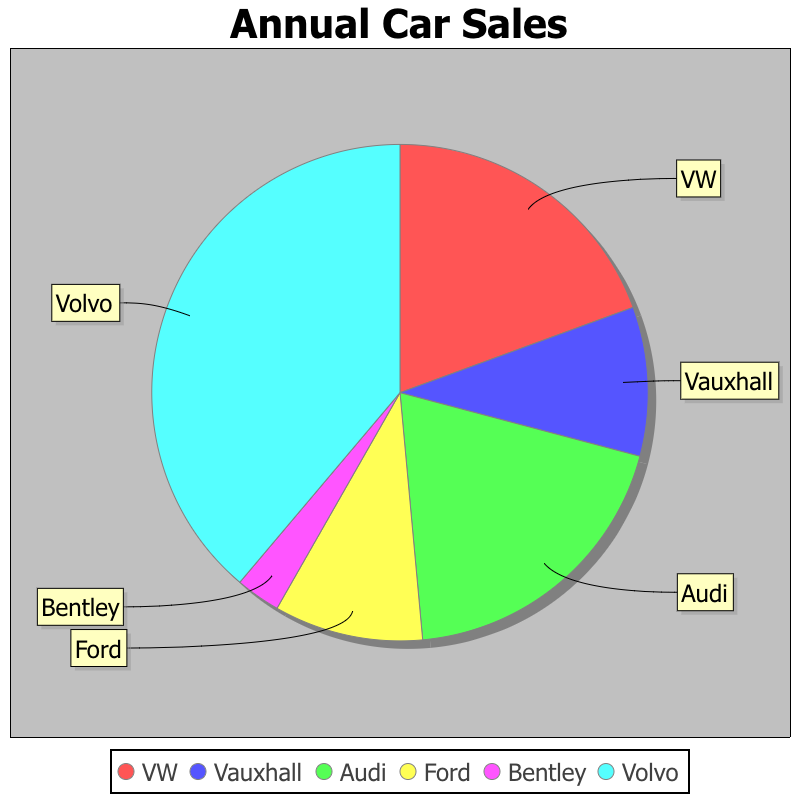
\includegraphics[width=0.8\columnwidth]{pie}
\end{center}

\subsection{Line Graphs}

\label{sec:lines}

Line graphs show data points:
\begin{ESL}
lgraph::Display = 
  LineGraph([],'Sales','Month','Volume',700,500,[
    GLine([],'Product' + i,[
      LPoint([],month,random(500)) | month <- 0..12 ]) 
    | i <- 0..3 ]);

edb <- Show('mylines',lgraph);
\end{ESL}
producing:
\begin{center}
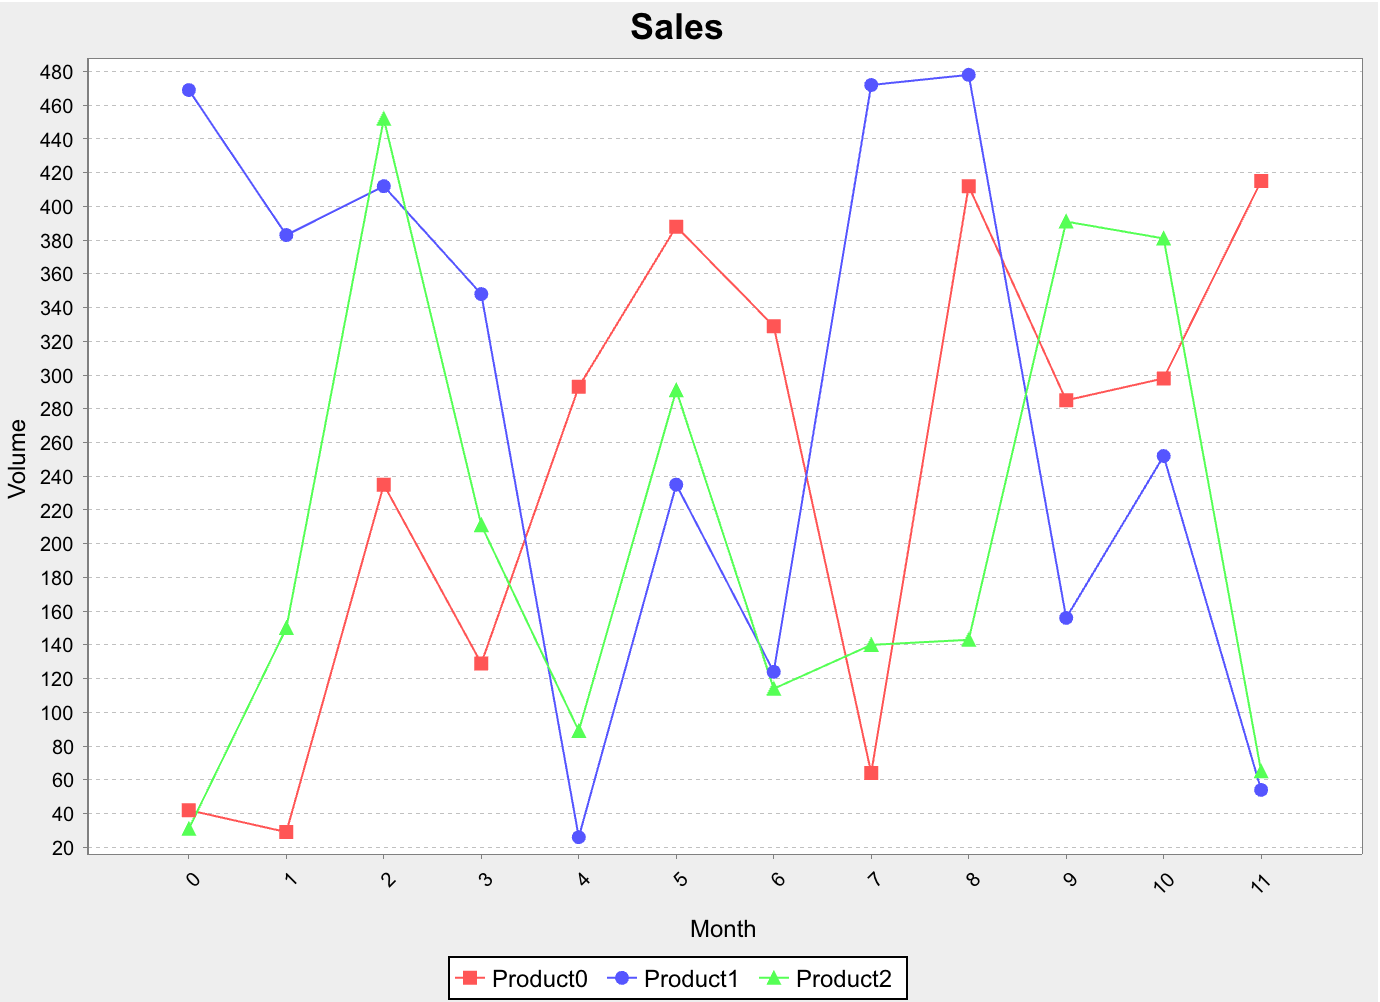
\includegraphics[width=\columnwidth]{lines}
\end{center}

\subsection{Pictures}

\label{sec:picture}

EDB provides a simple model of picture elements that map directly onto SVG. The following picture:
\begin{center}
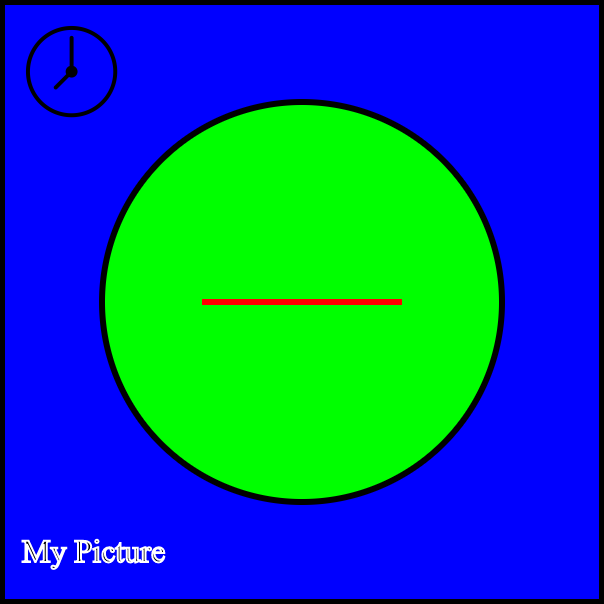
\includegraphics[width=0.6\columnwidth]{picture}
\end{center}
is produced by:
\begin{ESL}
picture::Display = Picture(500,500,[
  Rectangle(100,100,300,300,
    'fill:rgb(0,0,255);stroke-width:3;stroke:rgb(0,0,0)'),
  Circle(250,250,100,
    'fill:rgb(0,255,0);stroke-width:3;stroke:rgb(0,0,0)'),
  Line(200,250,300,250,
    'stroke-width:3;stroke:rgb(255,0,0)'),
  Image(110,110,50,50,
    'https://img.icons8.com/ios/1600/clock.png'),
  Text(110,380,'My Picture',
    'stroke:rgb(255,255,255)')
]);

edb <- Show('mypicture',picture);
\end{ESL}

\subsection{Graphs}

\label{sec:graphs}

EDB can display graphs using GraphViz. For example the following command:
\begin{ESL}
graph::Display = Graph([],[
  Node([],0,HTML('0')),
  Node([],1,HTML('1')),
  Node([],2,HTML('2')),
  Node([],3,HTML('3'))],[
  Edge([],0,1,HTML('e1')),
  Edge([],0,2,HTML('e2')),
  Edge([],1,3,HTML('e3')),
  Edge([],2,3,HTML('e4'))]);
  
edb <- Show('mygraph',graph);
\end{ESL}
produces the following display:
\begin{center}
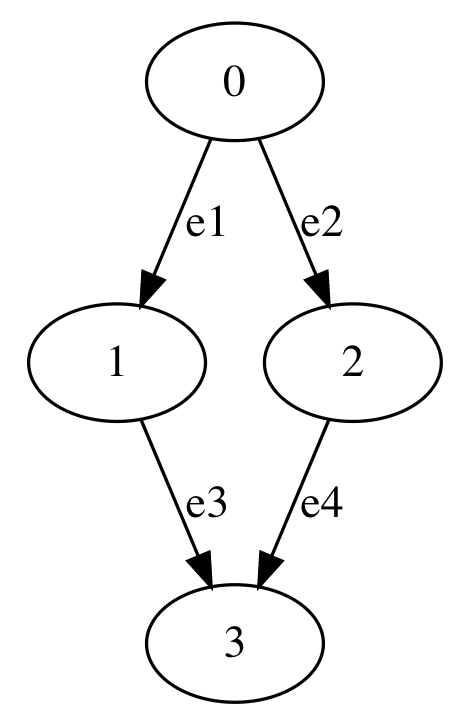
\includegraphics[height=4cm]{example_graph}
\end{center}

\begin{figure*}[t]
\begin{ESL}
export main;

import 'esl/lists.esl', 'esl/displays.esl';

nodeColour(n::Node)::Str = propValue(nodeProps(n),'fillcolor'); 
setNodeColour(n::Node,c::Str)::Node = setNodeProps(n,setProp(nodeProps(n),'fillcolor',c));
edgeBetween(e::Edge,n1::Node,n2::Node)::Bool = edgeTo(e,n1,n2) or edgeTo(e,n2,n1);
edgeTo(e::Edge,n1::Node,n2::Node)::Bool = edgeSource(e) = nodeId(n1) and edgeTarget(e) = nodeId(n2); 
edgeOn(e::Edge,n::Node)::Bool = edgeSource(e) = nodeId(n) or edgeTarget(e) = nodeId(n);

kempe(graph::Display,colours::[Str])::Display =
  // Simple algorithm to colour a planar graph.
  // This is taken from http://www.cs.princeton.edu/~appel/Color.pdf
  // graph must be planar and has no more than 3v - 6 edges.
  case graph {
    Graph(props,[],edges)    -> graph;
    Graph(props,nodes,edges) ->
      let degreeLessThan5(n::Node)::Bool = length[Edge]([ e | e <- edges, ?(edgeOn(e,n)) ]) <= 5; in
      let n::Node = select1[Node](nodes,null[Node],degreeLessThan5); in
      let es::[Edge] = [ e | e <- edges, ?(edgeSource(e) = nodeId(n) or edgeTarget(e) = nodeId(n)) ]; in
      let g::Display = kempe(Graph(props,remove[Node](n,nodes),removeAll[Edge](es,edges)),colours); 
      in case g {
           Graph(props,nodes,edges) ->
             let adjacent::[Node] = [ n0 | n0 <- nodes, ?(exists[Edge](fun(e::Edge)::Bool edgeBetween(e,n,n0),es)) ]; in
             let usedColours::[Str] = [ nodeColour(n) | n <- adjacent ]; in
             let available::[Str] = removeAll[Str](usedColours,colours);
             in Graph(props,setNodeColour(n,head[Str](available)):nodes,edges+es);
      }
  }

mkPlanar(v::Int)::Display = Graph([],
  [ Node([Prop('style','filled'),Prop('fillcolor','')],i,HTML('N' + i)) | i <- 0..v ],
  [ Edge([],source,target,HTML('')) | 
      i <- 0..random((3*v)-6), 
      source <- [random(v)], 
      target <- [random(v)], 
      ?(source <> target) ]);

act main::Act {} {
  -> edb <- Show('graph',kempe(mkPlanar(20),['red','green','blue','gold','deeppink']));
}
\end{ESL}
\caption{Graph Colouring}
\label{fig:graph_colouring}
\end{figure*}
Properties in graphs, nodes and edges are used to control GraphViz. 
Figure \ref{fig:graph_colouring} shows an example of EDB displays being used to create planar graphs and then colour the nodes. Any planar graph can be coloured using no more than 5 colours using Kempe's algorithm. The node properties are used to set the fill colour. The following is an example output:
\begin{center}
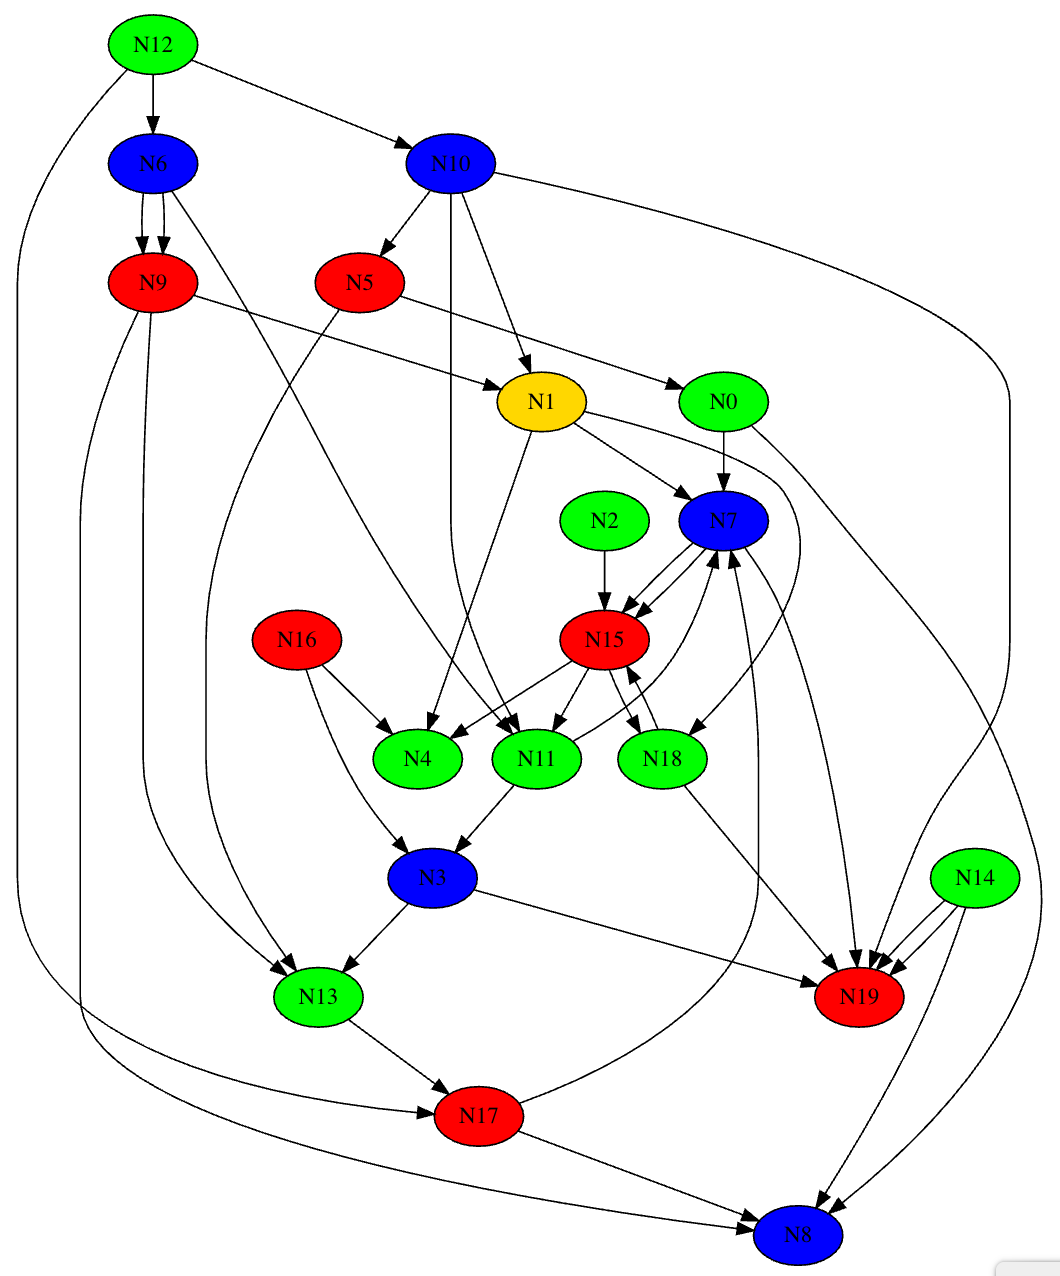
\includegraphics[width=0.9\columnwidth]{graph_colour}
\end{center}

\subsection{Filmstrips}

\label{sec:filmstrips}

An EDB  {\it filmstrip} is a list of displays that are shown on an EDB tab with a slider. When the slider is moved, the tab is updated to show the display at the appropriate index in the list. The following shows a sequence of line graphs where the slider can be moved to a month causing the graph to show the sales up to and including that month:
\begin{center}
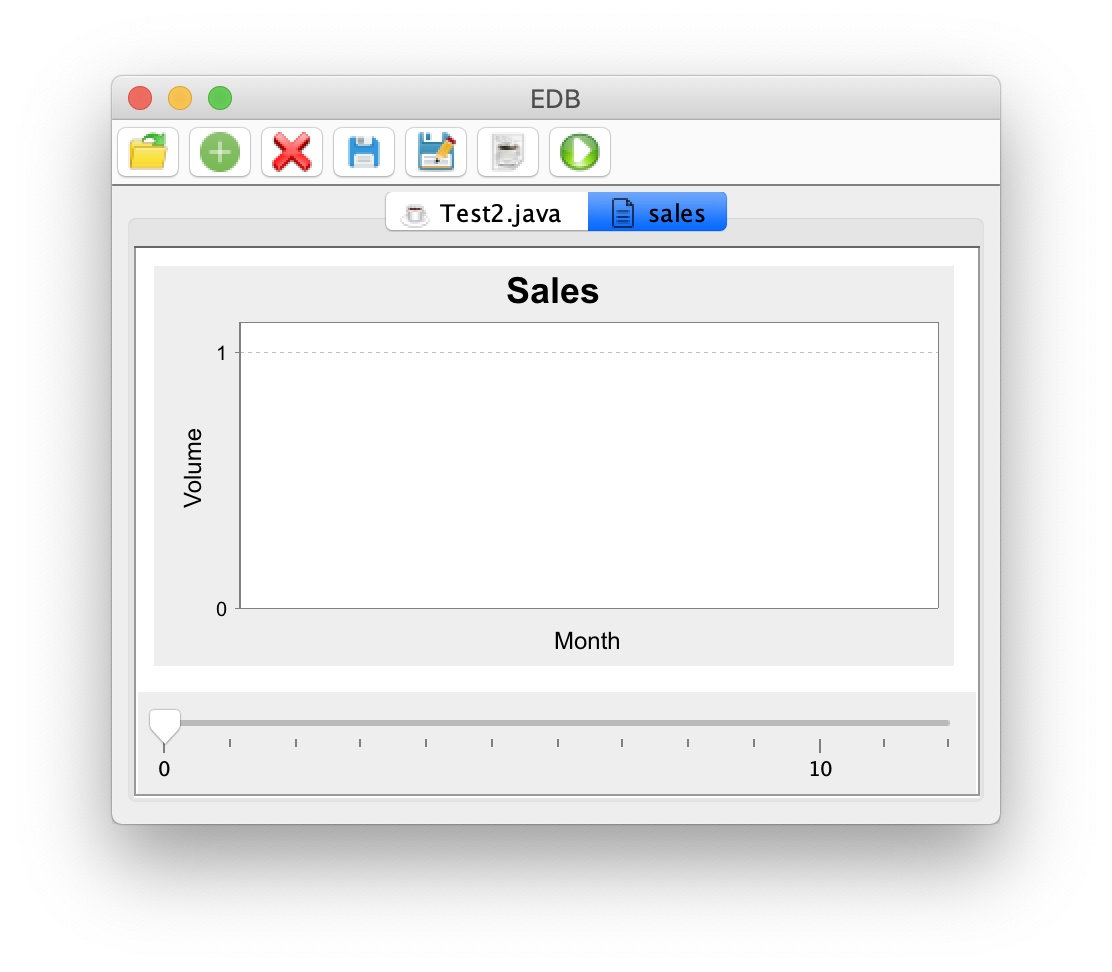
\includegraphics[width=0.9\columnwidth]{film1}
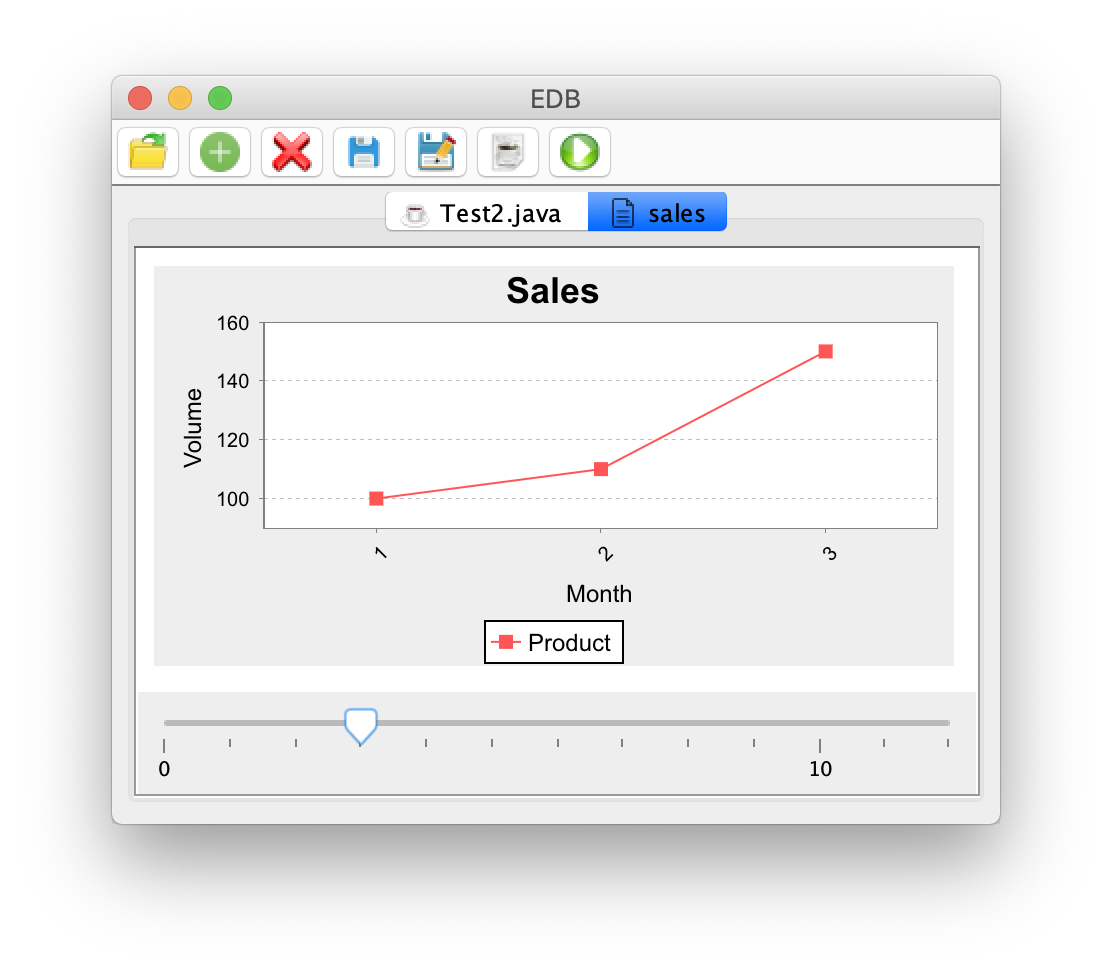
\includegraphics[width=0.9\columnwidth]{film2}
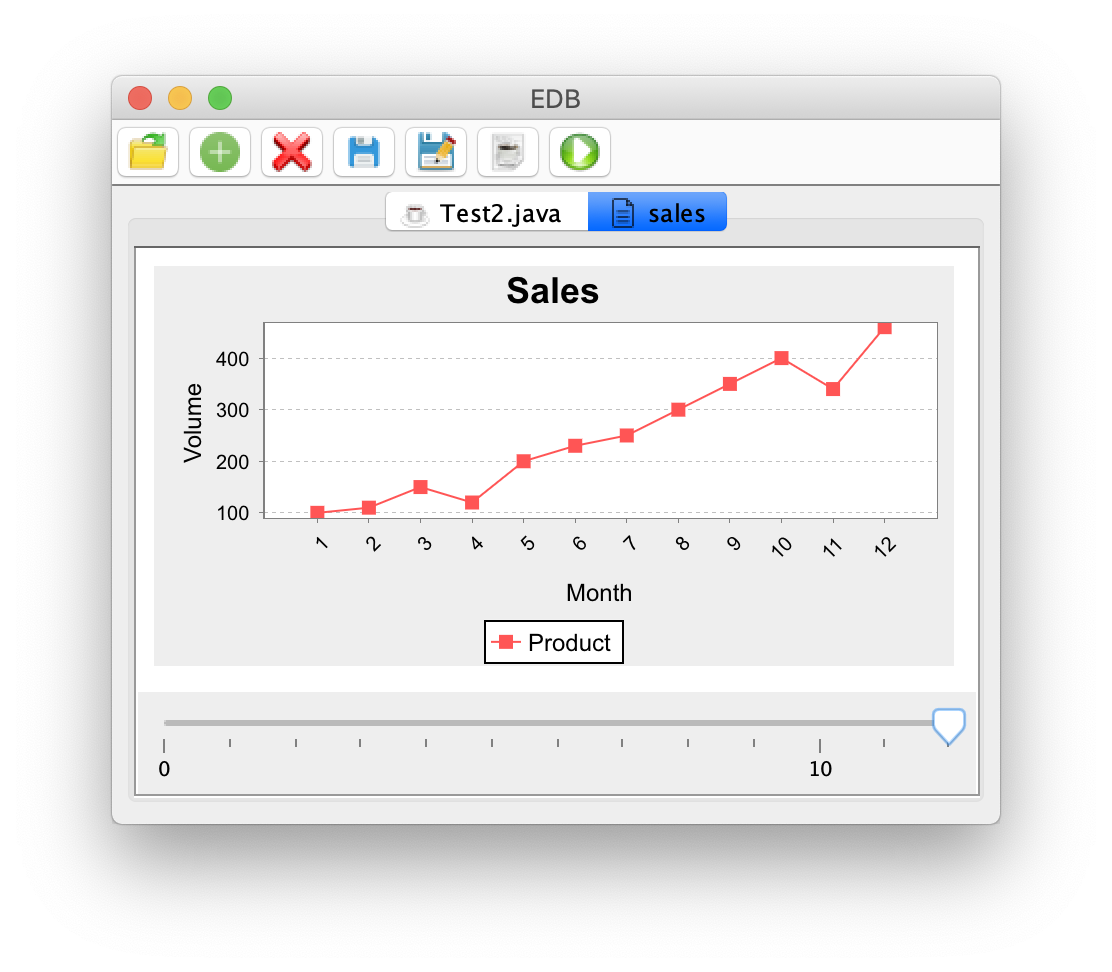
\includegraphics[width=0.9\columnwidth]{film3}
\end{center}
The filmstrip is generated as follows:
\begin{ESL}
data Sale = Sale(Int,Int);

salesFigures::[Sale] = [
  Sale(1,100),
  Sale(2,110),
  Sale(3,150),
  Sale(4,120),
  Sale(5,200),
  Sale(6,230),
  Sale(7,250),
  Sale(8,300),
  Sale(9,350),
  Sale(10,400),
  Sale(11,340),
  Sale(12,460)];
  
  
lgraphs::[Display] = [ 
  LineGraph([],'Sales','Month','Volume',400,200,[
    GLine([],'Product',[ LPoint([],m,s) 
    | Sale(m,s) <- take[Sale](salesFigures,month)
    ])
  ]) | month <- 0..13 ];
  
edb <- Filmstrip('sales',lgraphs);
\end{ESL}

\subsection{Sequence Diagrams}

\label{sec:sequence_diagram}

Sequence diagrams are a useful way of visualising the dynamic progress of an application. For example, sequential factorial is usually defined recursively so that each calculation of $!n$ waits on the stack until the calculation of $!(n-1)$ returns. Concurrent factorial can use actors to implement that stack frames that are waiting for results and allow any number of factorial calculations to occur at the same time. This is done as follows:
\begin{ESL}
type Customer = Act { Value(Int,Int,Int); }
type Fact = Act{ Get(Int,Int,Int,Customer); }

act fact::Fact {
  Get(0,c) -> {
    c <- Value(1);
  }
  Get(n,c) -> 
    let cc::Customer = new cust(n,c);
    in self <- Get(n-1,cc);
}

act cust(n::Int,c::Customer)::Customer {
  Value(m) -> c <- Value(n*m);
}

act main::Customer {
  f::Fact = new fact;
  -> {
    fact <- Get(3,self);
    fact <- Get(3,self);
  }
  Value(n) ->  print[Str]('result = ' + n);
}
\end{ESL}
When \code{fact} is send a request to calculate a factorial, it tests whether the supplied value is \code{0}. If so, it immediately replies to the customer \code{c} supplying \code{1}. Otherwise, the supplied value is \code{n} and the factorial actor sends itself a message to calculate \code{!n-1} and to reply to a newly created customer. 

Although this is recursive, it does not prevent interleaving of factorial requests. This can be seen if we create a sequence diagram for two different factorial calculations:
\begin{center}
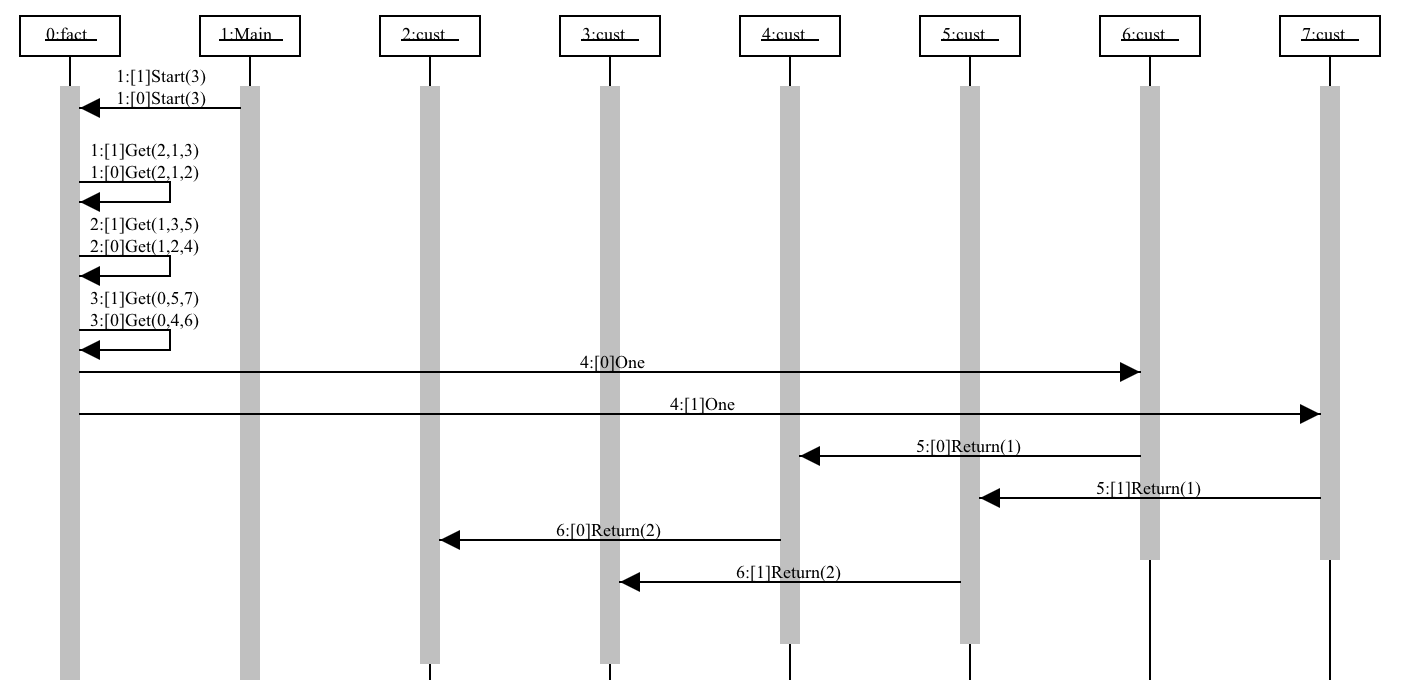
\includegraphics[width=\columnwidth]{sequence}
\end{center}
The diagram is produced by creating an EDB sequence diagram. Each factorial documents its progress as a sequence of messages tagged with an identifier that designates its thread of execution (shown as \code{[0]} and \code{[1]} on the diagram. Once the factorials are completed, a value of the form \code{Sequence(actors,messages)} is created and displayed where \code{actors} contains a representation of all the actors involved in the calculation and \code{messages} is a list of messages sent between them. The ESL code is shown below:
\begin{ESL}
type Customer = Act { export id::Int; Value(Int,Int,Int);}
type Fact = Act{ export id::Int; Get(Int,Int,Int,Customer);}

data M =
  GetValue(Int,Int,Int,Fact,Fact,Customer,Customer)
| ReturnValue(Int,Int,Int,Customer,Customer)
| Zero(Int,Int,Fact,Customer)
| Start(Int,Int,Customer,Fact);

actors::[Actor] = [];
messages::[M] = [];

addActor(behaviour::Str)::Int =
  grab(actors) {
    let id::Int = length[Actor](actors);
    in {
      actors := actors + [Actor(id,0,timeOut,behaviour)];
      id;
    }
  }
  
act fact::Fact {
  export id;
  id::Int = 0;
  -> id := addActor('fact');
  Get(0,thread,time::Int,c::Customer) -> grab(messages) {
    messages := messages + [Zero(thread,time,self,c)];
    c <- Value(thread,time+1,1);
  }
  Get(n::Int,thread,time::Int,c) -> {
    let cc::Customer = new cust(n,c);
    in grab(messages) {
      messages := messages + 
        [GetValue(n-1,thread,time,self,self,c,cc)];
      self <- Get(n-1,thread,time+1,cc);
    }
  }
}

act cust(n::Int,c::Customer)::Customer {
  export id;
  id::Int = 0;
  -> id := addActor('cust');
  Value(thread,time::Int,m::Int) -> grab(messages) {
    messages := messages + 
      [ReturnValue(n*m,thread,time,self,c)];
    setDeath(id,time);
    c <- Value(thread,time+1,n*m);
  }
}

translate(m::M)::Message =
  case m {
    [] -> [];
    Start(n,id,c,f) -> 
      Message(1,c.id,f.id,'['+id+']Start('+n+')');
    GetValue(n,id,t,src,tgt,srcC,tgtC) -> 
      Message(t,src.id,tgt.id,
        '['+id+']Get('+n+','+srcC.id+','+tgtT.id+')');
    ReturnValue(n,id,t,src,tgt) -> 
      Message(t,src,tgt.id,'['+id+']Return(' + n + ')');
    Zero(id,t,f,c) -> 
      Message(t,f.id,c.id,'['+id+']One');
  }
  
getActor(id::Int,as::[Actor])::Actor =
  case as {
    Actor(i,time,death,b):l when i = id -> 
      Actor(i,time,death,b);
    a:l -> getActor(id,l);
  }
  
changeDeath(a::Actor,t::Int)::Actor =
  case a {
    Actor(i,birth,death,b) ->  Actor(i,birth,t,b);
  }
  
setDeath(id::Int,time::Int)::Void =
  let oldActor::Actor = getActor(id,actors); in
  let newActor::Actor = changeDeath(oldActor,time);
  in grab(actors) {
   actors := subst[Actor](newActor,oldActor,actors);
  }

act main::Customer {
  export id;
  id::Int = 0;
  counter::Int = 0;
  count::Int = 1;
  f::Fact = new fact;
  numberOfFacts::Int = 2;
  computeFact(n::Int)::Void = grab(messages)) {
    messages := messages + [Start(n,counter,self,f)];
    counter := counter + 1;
    f <- Get(n,counter-1,1,self);
  }
  -> {
    id := addActor('Main');
    computeFact(3);
    computeFact(3);
  }
  Value(threadId::Int,time::Int,n::Int) -> {
    setDeath(id,time);
    if count = numberOfFacts
    then {
      edb <- Show('Factorial',Sequence(actors,[ 
        translate(m) | m <- messages 
      ]));
      stopAll();
    } else count := count + 1;
  }
}

\end{ESL}

\subsection{Combining Pictures}

\label{sec:combination}

The \code{Display} data type allows pictures to be combines using trees. A tree consists of a collection of h-boxes and v-boxes that EDB will auto-layout. These are similar to HTML tables, but the size of the tree can be controlled. The following example shows how a filmstrip of trees can be constructed to create a simple predator-prey application. The predator-prey world consists of marked locations:
\begin{ESL}
data Location = 
  EmptyLoc 
| PredLoc 
| PreyLoc 
| Rock;
\end{ESL} 
Predators and prey, are located at points in the world and can be requested to move:
\begin{ESL}
Act Predator { 
  export getX::()->Int; 
         getY::()->Int; 
         at::(Int,Int)->Bool; 
         getId::()->Int; 
  Move; 
}
Act Prey { 
  export getX::()->Int; 
         getY::()->Int; 
         at::(Int,Int)->Bool; 
  Move; 
}
\end{ESL}
The board is a nested list of locations that is set up at random:
\begin{ESL}
data Point          = Point(Int,Int);
pointX(p::Point)::Int = case p { Point(x,y) -> x; }
pointY(p::Point)::Int = case p { Point(x,y) -> y; }
board::[[Location]]  = [];
rocks::[Point]       = drop[Point](points,numOfPredators+1);
points::[Point]      = 
  letrec generate(ps::[Point],n::Int)::[Point] = 
    if n = 0
    then [];
    else 
      let x::Int = random(width); 
          y::Int = random(height); 
      in if member[Point](Point(x,y),ps) 
         then generate(ps,n); 
         else Point(x,y):generate(Point(x,y):ps,n-1);
  in generate([],numOfPredators+1+numOfRocks);
\end{ESL}
Control of positions uses the following predicates:
\begin{ESL}
onBoard(x::Int,y::Int)::Bool = 
  (x >= 0) and (x < width) and (y >= 0) and (y < height);
onRock(x::Int,y::Int)::Bool = 
  member[Point](Point(x,y),rocks);
legalPreyPos(x::Int,y::Int)::Bool = 
  (not(onRock(x,y))) and onBoard(x,y) and 
  not(exists[Predator](fun(p::Predator)::Bool 
    p.at(x,y),predators));
legalPredatorPos(x::Int,y::Int)::Bool = 
  (not(onRock(x,y))) and onBoard(x,y) and 
  (not(exists[Predator](fun(p::Predator)::Bool 
    p.at(x,y),predators))) and 
  not(thePrey.at(x,y));
\end{ESL}
When they make a move, each of the actors in the world save their activity as a message on a global list. This will be used to create a graphical display of each snapshot of the world and eventually turned into a filmstrip:
\begin{ESL}
data Message = 
  MovePredator(Int,Int,Int) 
| MovePrey(Int,Int);
messages::[Message] = [];
\end{ESL}
A predator moves towards the prey. The variable \code{turn} is used to achieve equitable movement:
\begin{ESL}
act predator(id::Int,x::Int,y::Int)::Predator {
  export getX, getY, at, getId;
  getX()::Int = x;
  getY()::Int = y;
  getId()::Int = id;
  at(px::Int,py::Int)::Bool = (px = x) and (py = y);
  
  move(dx::Int,dy::Int)::Void = {
    if legalPredatorPos(x+dx,y+dy)  
    then { 
      x := x + dx;
      y := y + dy;
      messages := messages + [MovePredator(id,x,y)];
    } else { }
  }

  Move -> grab(messages) { 
    if turn = id
    then {
      turn := (turn + 1) % (numOfPredators+1);
      let dx::Int = 
            if thePrey.getX() > x 
            then 1; 
            else if thePrey.getX() < x 
            then - 1; 
            else 0;
          dy::Int = 
            if thePrey.getY() > y 
            then 1; 
            else if thePrey.getY() < y 
            then -1; 
            else 0;
      in { 
        if (dy <> 0) and legalPredatorPos(x,y+dy)
        then move(0,dy);
        else if (dx <> 0) and legalPredatorPos(x+dx,y)
        then move(dx,0);
        else probably(50) {
          move(0,1-random(3)); 
        } else move(1-random(3),0);
      }
    } else {}
  }
}
\end{ESL}
The predators are created in a list:
\begin{ESL}
predators::[Predator] = [ 
  new predator(p,pointX(nth[Point](points,p)),pointY(nth[Point](points,p))) 
| p::Int <- 0..numOfPredators 
];
\end{ESL}
The prey moves away from the predators. Unlike the predators, the prey can move diagonally:
\begin{ESL}
act prey(x::Int,y::Int)::Prey {

  export getX, getY, at;
  
  getX()::Int = x;
  getY()::Int = y;
  
  at(px::Int,py::Int)::Bool = (px = x) and (py = y);
  dir(n::Int)::Int         = if n < 0 then -1; else 1;
  
  dirX::Int = 1 - random(3);
  dirY::Int = 1 - random(3);
  
  move(dx::Int,dy::Int)::Void = grab(messages) {
    if legalPreyPos(x+dx,y+dy)
    then {
      x := x + dx;
      y := y + dy;
      messages := messages + [MovePrey(x,y)];
    } else { }
  }
  
  predatorWins()::Void = {
    print[Str]('predator wins!');
    stop := true;
  }
  
  legalMoves()::[Point] = [ Point(dx,dy) | 
    dx <- [-1,0,1], 
    dy <- [-1,0,1], 
    ?(dx <> 0 or dy <> 0), 
    ?legalPreyPos(x+dx,y+dy) 
  ];
    
  changeDir()::Void = 
    case legalMoves() {
      Point(dx,dy):ps -> { dirX := dx; dirY := dy; }
      []              -> {}
    }

  Move -> grab(messages) { 
    if turn = numOfPredators
    then {
      turn := (turn + 1) % (numOfPredators+1);
      if legalMoves() = []
      then predatorWins();
      else if legalPreyPos(x+dirX,y+dirY)
      then move(dirX,dirY);
      else changeDir();
    } else {}
  }
}
\end{ESL}
A single prey is created:
\begin{ESL}
thePrey::Prey = 
  let x::Int = pointX(nth[Point](points,numOfPredators));
      y::Int = pointY(nth[Point](points,numOfPredators));
  in new prey(x,y);
\end{ESL}
At this point we have sufficient to run the world and send all actors a \code{Move} message. A sequence of messages can be transformed into a snapshot where the occupied locations. The snapshots can be merged and the resulting composite snapshots merged using \code{mapBoard}:
\begin{ESL}
mapMessage(m::Message)::[[Location]] = 
  case m {
    MovePredator(i,x0,y0) ->
     [[ if (x=x0) and (y=y0) 
        then PredLoc 
        else if onRock(x,y) 
        then Rock 
        else EmptyLoc 
      | x <- 0..width ] 
     | y <- 0..height ];
    MovePrey(x0,y0) ->
      [[ if (x=x0) and (y=y0) 
         then PreyLoc 
         else if onRock(x,y) 
         then Rock 
         else EmptyLoc 
       | x <- 0..width ] 
      | y <- 0..height ];
  }

mapBoard(b::[[Location]])::Display =
  let mapRow(row::[Location])::TreeElement = 
        HBox([],[ 
          case l { 
            PredLoc -> predIcon; 
            PreyLoc -> preyIcon; 
            EmptyLoc ->space; 
            Rock -> rockIcon; } | l <- row ]);
  in Tree(width*size,height*size,
       VBox([],[ 
         mapRow(nth[[Location]](b,y)) | y <- 0..height ]));
\end{ESL}
The resulting list of displays is then presented as a filmstrip. The following shows steps in an example filmstrip:
\begin{center}
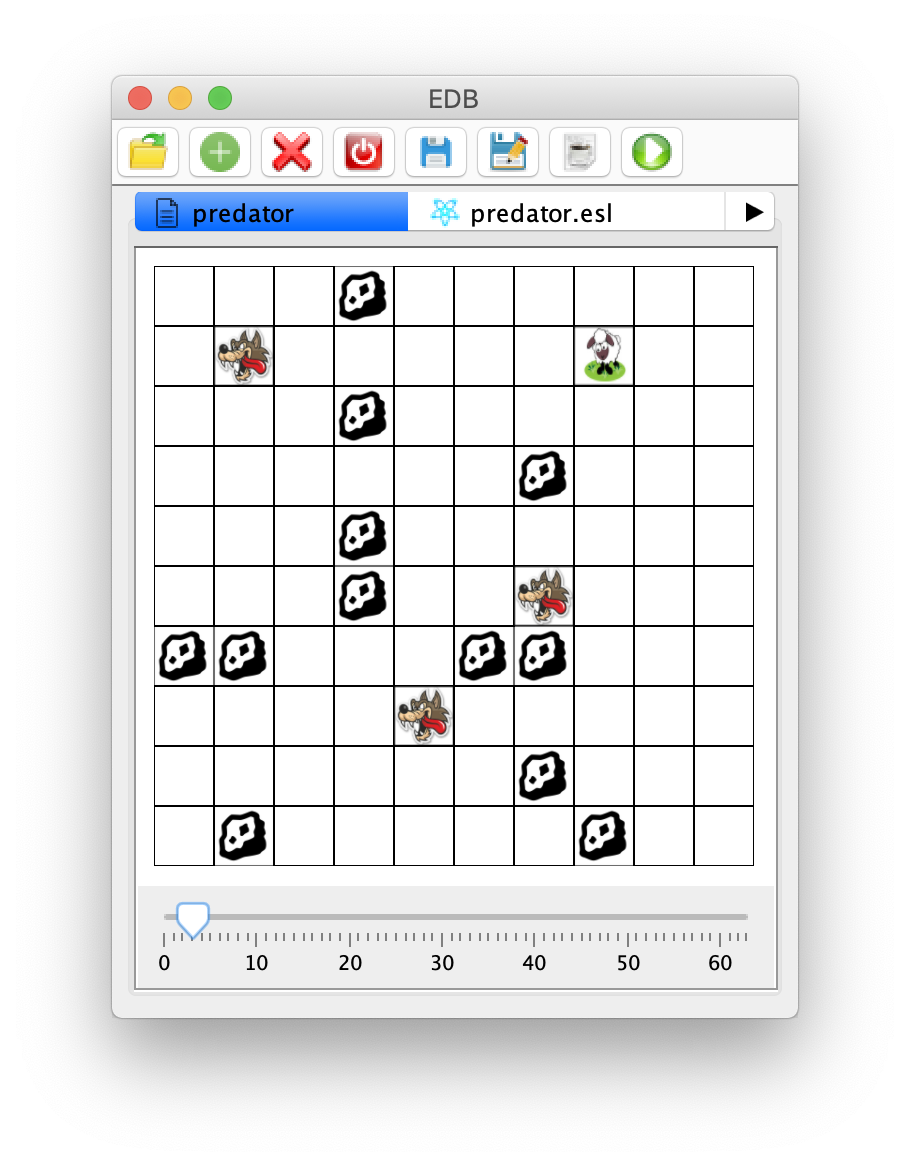
\includegraphics[width=\columnwidth]{pred1}
\end{center}
\begin{center}
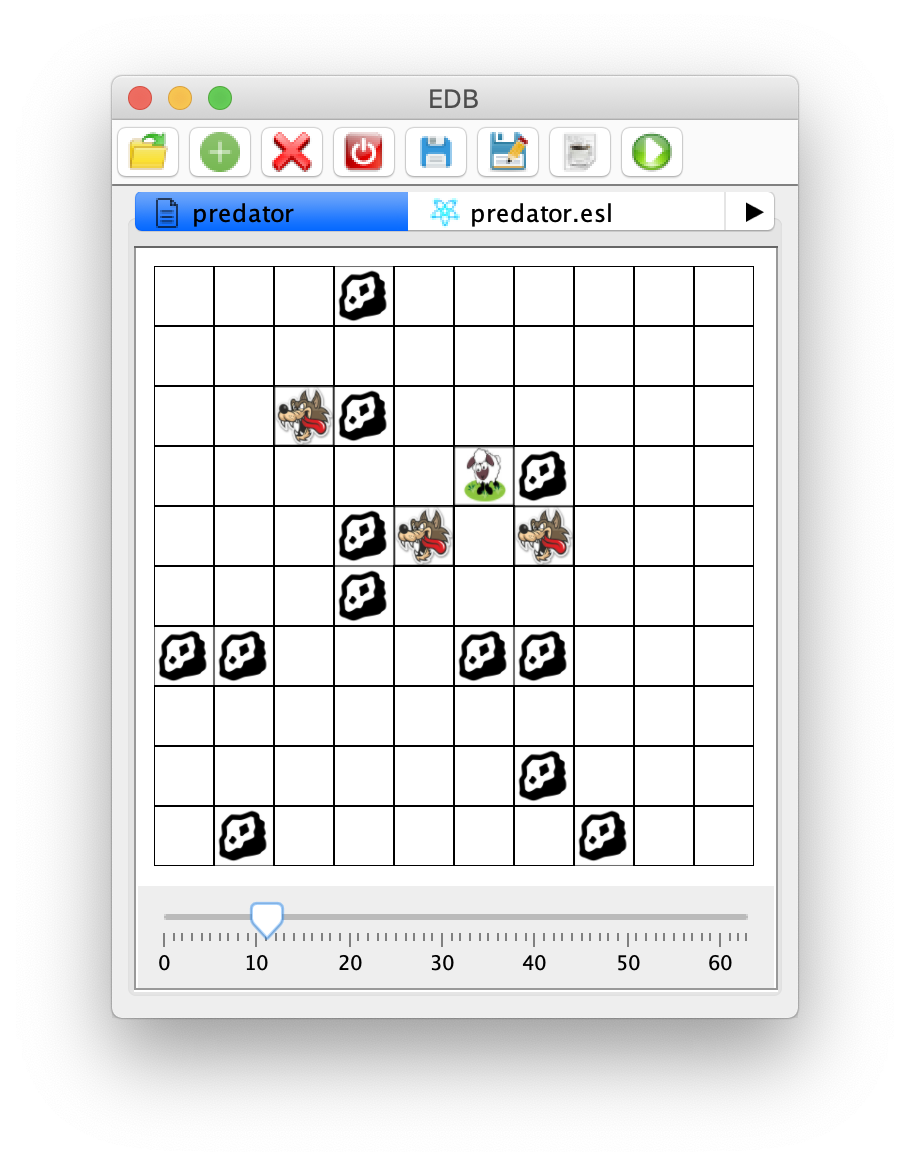
\includegraphics[width=\columnwidth]{pred2}
\end{center}
\begin{center}
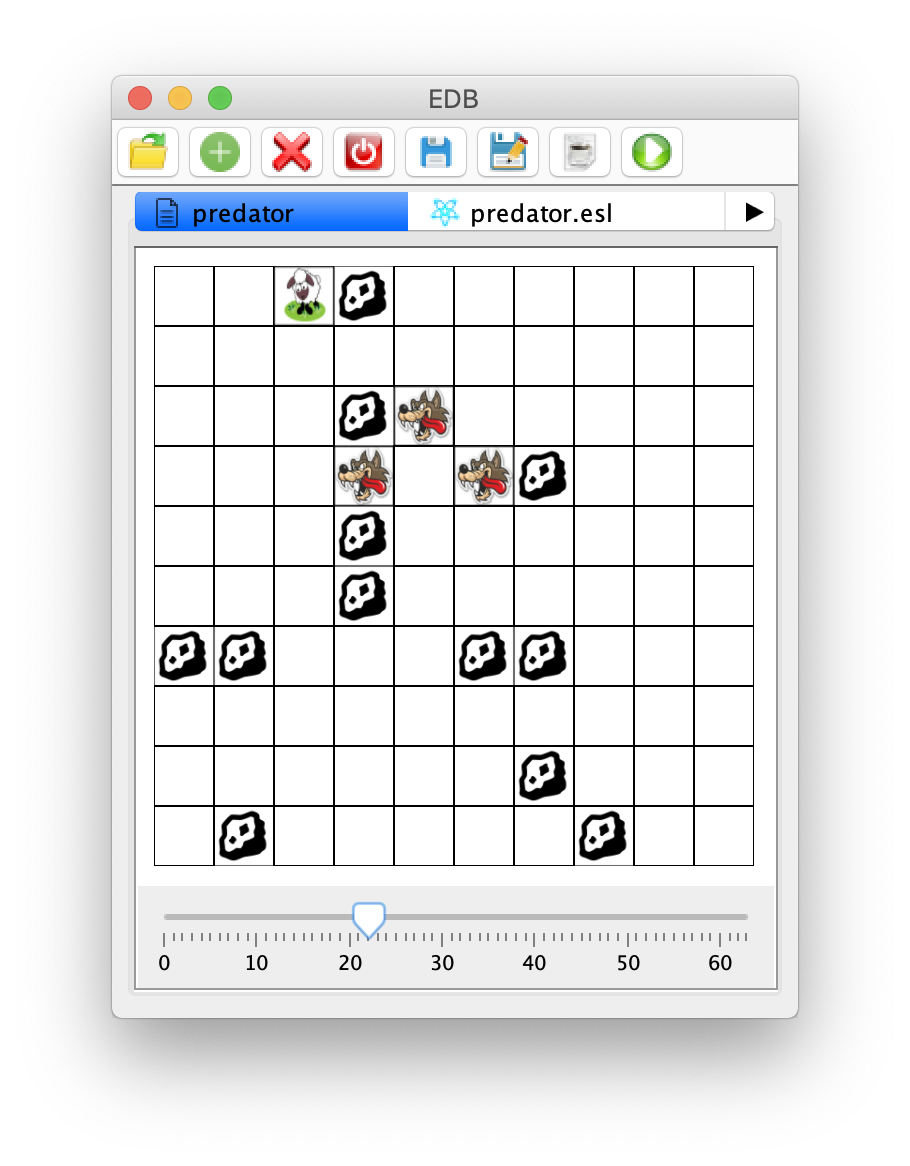
\includegraphics[width=\columnwidth]{pred3}
\end{center}
\begin{center}
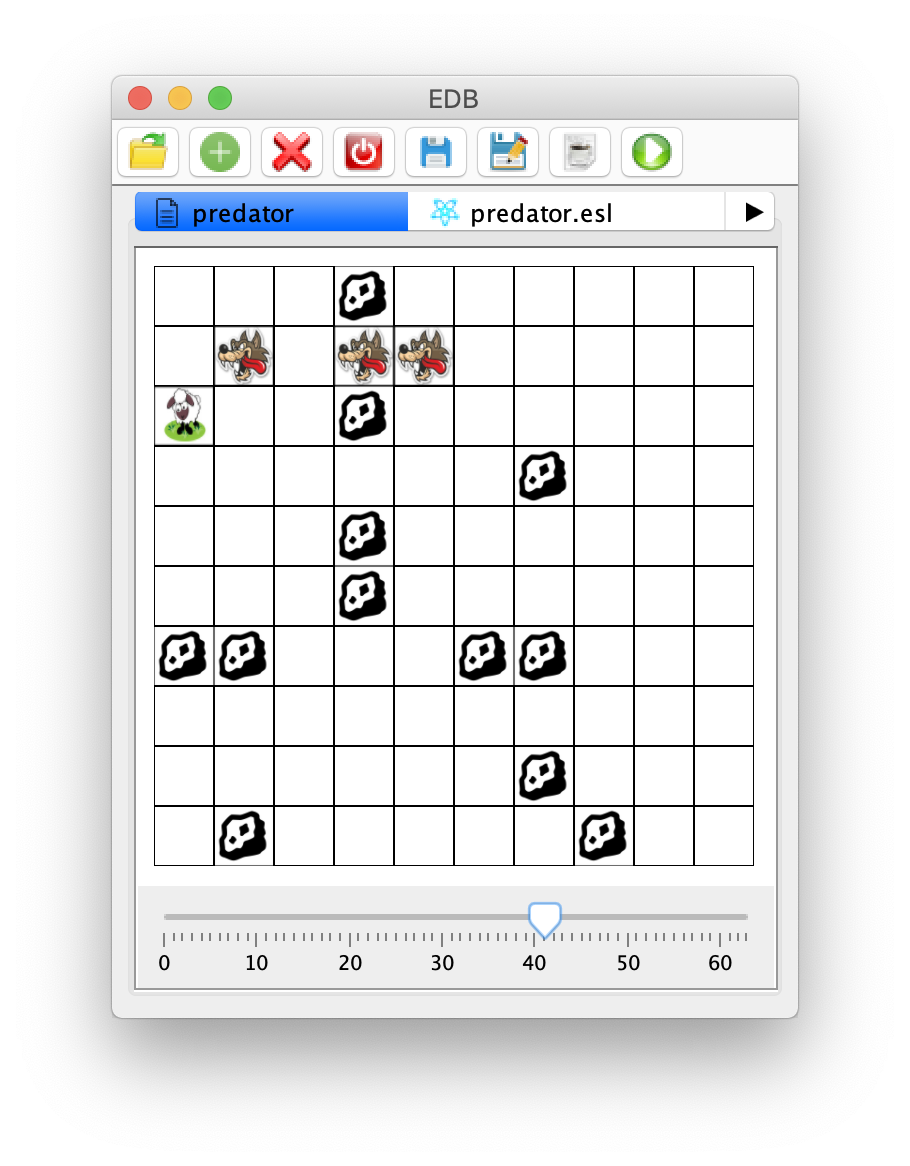
\includegraphics[width=\columnwidth]{pred4}
\end{center}

\section{Java Interface}

\label{sec:java_interface}

An instance of such a class is created in ESL using \code{new} and registered with EDB using:
\begin{ESL}
edb.display::Forall[T] (Str,T) -> Void
\end{ESL}
for example: \code{edb.display[G]('TabName',graphics)}

\section{Compilation}

\label{sec:compilation}

This section will describe the compilation process and the Java constructs produced by the ESL compiler.

\section{Implementation}

\label{sec:implementation}

This section will describe the Java libraries that support ESL.

\bibliography{bibv4}

\clearpage

\appendix

\renewcommand*{\thesection}{\Alph{section}}

\section{Syntax and Type Checking}

\label{sec:syntax}

\begin{comment}

\begin{figure*}
\begin{tabular}{l|l}
\hline
\begin{minipage}{.275\textwidth}
\footnotesize
{\it Syntax}:\\
\begin{tabular}{llr}
t ::= & & {\it terms}\\
& {\tt x} & {\it variable}\\
& {\tt {\bf new}(t)}& {\it creation}\\
& $\lambda$(\={d}) t&{\it function}\\
& {\tt {\bf act} \{ \={d} \={h} \}}&{\it behaviour}\\
& n & {\it number}\\
& s & {\it string} \\
& b & {\it boolean}\\
& {\bf grab}(x) t & {\it lock}\\
& {\bf if} t {\bf then} t {\bf else} t& {\it conditional}\\
& t $\leftarrow$ t&{\it send}\\
& {\bf case} t \{ \={h} \}&{\it projection}\\
& [\={t}]&{\it list}\\
& t(\={t}) & {\it application}\\
& t[\={T}]& {\it type application}\\
& C(\={t}) & {\it injection}\\
i ::= & d=t& {\it initialisation}\\
d ::= & x[\={X}]::T& {\it declarations}\\
h ::= & C(\={x}) $\rightarrow$ t&{\it handlers}\\
T ::= & & {\it types}\\
& {\bf Int} & {\it integer type}\\
& {\bf Bool} & {\it boolean type}\\
& {\bf Str} & {\it string type}\\
& $\forall$ \={X} . T & {\it universal}\\
& X & {\it variable}\\
& {\bf Union} \{ \={m} \}&{\it union}\\
& {\bf Act} \{ \={d} \={m} \} & {\it behaviour}\\
& (\={T}) $\rightarrow$ T & {\it function type}\\
m ::= & C(\={T}) & {\it message type}\\
\end{tabular}
\end{minipage}
&
\begin{minipage}{0.7\textwidth}
\footnotesize
{\it Type Checking}:\\
\[\begin{array}{cc}
\begin{array}{cr}
\inference{{\tt x::T}\in\Gamma}{\Gamma\vdash{\tt x::T}}&\text{T-VAR}\\\\
\inference{\Gamma\vdash{\tt t}::\text{\tt {\bf Act} \{ \={d} \={m} \}}}{\Gamma\vdash{\tt {\bf new}(t)} :: \text{\tt {\bf Act} \{ \={d} \={m} \}}}&\text{T-NEW}\\\\
\inference{\Gamma,\text{\={x}::\={T}}\vdash\text{t::T}}{\Gamma\vdash\text{$\lambda$(\={d}) t::(\={T})$\rightarrow$T}}&\text{T-FUN}\\\\
%
\Gamma\vdash\text{\tt {\bf act} \{ \={d} \={m} \}::{\bf Act} \{ \={d} \={m} \}}&\text{T-ACT}\\\\
\inference{\Gamma\vdash\text{t\textsubscript{1}::{\bf Act} \{ \={d} \={m} \}}\\\Gamma\vdash\text{t\textsubscript{2}::{\bf Union} \{ \={m} \}}}{\Gamma\vdash\text{t\textsubscript{1}$\leftarrow$ t\textsubscript{2}::{\bf Union} \{ \={m} \}}}&\text{T-SEND}\\\\
%
\Gamma\vdash\text{\tt n::{\bf Int}}&\text{T-INT}\\\\
\Gamma\vdash\text{\tt s::{\bf Str}}&\text{T-STR}\\\\
\Gamma\vdash\text{\tt b::{\bf Int}}&\text{T-BOOL}\\\\
\inference{\Gamma\vdash\text{\tt t::T}}{\Gamma\vdash\text{\tt{\bf grab}(x) t :: T}}&\text{T-LOCK}\\\\
\inference{\Gamma\vdash\text{\tt t\textsubscript{1}::Bool}\\\Gamma\vdash\text{\tt t\textsubscript{2},t\textsubscript{3}::T}}{\Gamma\vdash\text{\tt{\bf if} t\textsubscript{1} {\bf then} t\textsubscript{2} {\bf else} t\textsubscript{3} :: T}}&\text{T-IF}
\end{array}
&
\begin{array}{cr}
\inference{
\Gamma\vdash{\tt {\bf case}\ t\ \{ \text{\={m}}\textsubscript{1} \} :: T}\\
\Gamma\vdash{\tt {\bf case}\ t\ \{ \text{\={m}}\textsubscript{2} \} :: T}}
{
\Gamma\vdash{\tt {\bf case}\ t\ \{ \text{\={m}}\textsubscript{1},\text{\={m}}\textsubscript{2} \} :: T}}&\text{T-CASE1}\\\\
\inference{
\Gamma\vdash{\tt t\textsubscript{1} :: {\bf Union} \{ \text{\={m}},C(\text{\={T}}) \}}\\
\Gamma,{\tt\text{\={x}}::\text{\={T}}\vdash t\textsubscript{2}::T}}{
\Gamma\vdash{\tt {\bf case}\ t\textsubscript{1}\ \{ C(\text{\={x}}) \rightarrow t\textsubscript{2} \} :: T}}&\text{T-CASE2}\\\\
\Gamma\vdash{\tt [] :: \forall X. [X]}&\text{T-NIL}\\\\
\inference{\Gamma\vdash{\tt [\text{\={t}}\textsubscript{1}] :: [T]}\\\Gamma\vdash{\tt [\text{\={t}}\textsubscript{2}] :: [T]}}{
\Gamma\vdash\text{[\={t}\textsubscript{1},\={t}\textsubscript{2}] :: [T]}}&\text{T-LIST1}\\\\
\inference{\Gamma\vdash{\tt t::T}}{\Gamma\vdash{\tt[t]::[T]}}&\text{T-LIST2}\\\\
\inference{\Gamma\vdash{\tt \text{\={t}}::\text{\={T}}}\\\Gamma\vdash{\tt t::(\text{\={T}})\rightarrow T}}{
\Gamma\vdash{\tt t(\text{\={t}})::T}}&\text{T-APP}\\\\
\inference{\Gamma\vdash{\tt t::\forall\text{\={X}}.T}}{\Gamma\vdash{\tt t[\text{\={T}}]::T[\text{\={T}}/\text{\={X}}]}}&\text{T-TAPP}\\\\
\inference{\Gamma,{\tt C(\text{\={T}})}\mapsto{\tt {\bf Union} \{ \text{\={m}} \}}\\
\Gamma\vdash{\tt \text{\={t}}::\text{\={T}}}}{\Gamma\vdash{\tt C(\text{\={t}})::{\bf Union} \{ \text{\={m}} \}}}&\text{\tt T-INJ}\\\\
\end{array}
\end{array}\]
\end{minipage}
\\
\hline
\end{tabular}
\caption{ESL Syntax and Type Checking}
\label{fig:ESL_type_checking}
\end{figure*}

\end{comment}

\section{Displays}

\label{sec:display_definitions}

\begin{ESL}
data Property = Prop(Str,Str);
type Props    = [Property];

propValue(props::Props,n::Str)::Str = 
  case props { 
    ps1 + [Prop(m,v)] + ps2 when m = n -> v; 
  }
  
hasProp(props::Props,n::Str)::Bool = 
  case props { 
    ps1 + [Prop(m,v)] + ps2 when m = n -> true; 
    props -> false; 
  }
  
setProp(props::Props,n::Str,v::Str)::Props = 
  case props { 
    ps1 + [Prop(m,v0)] + ps2 when m = n -> 
      ps1 + [Prop(n,v)] + ps2; 
  }


data PictureElement = 
  Rectangle(Int,Int,Int,Int,Str)
| Circle(Int,Int,Int,Str)
| Line(Int,Int,Int,Int,Str)
| Image(Int,Int,Int,Int,Str)
| Text(Int,Int,Str,Str);

data TreeElement = 
   TreeNode(PictureElement)
|  VBox(Props,[TreeElement])
|  HBox(Props,[TreeElement])
|  Padding(Props)
|  LabelledTree(Str,TreeElement);

data LinePoint = LPoint(Props,Int,Int);
data Row       = Row(Props,[Data]);
data Data      = Data(Props,Display);
data Slice     = Slice(Props,Str,Int);
data GLine     = GLine(Props,Str,[LinePoint]);
data Message   = Message(Int,Int,Int,Str);
data Actor     = Actor(Int,Int,Int,Str);
data Node      = Node(Props,Int,Display);
data Edge      = Edge(Props,Int,Int,Display);

edgeSource(e::Edge)::Int  = case e { Edge(ps,s,t,d) -> s; }
edgeTarget(e::Edge)::Int  = case e { Edge(ps,s,t,d) -> t; }
nodeId(n::Node)::Int      = case n { Node(ps,id,d) -> id; }
nodeProps(n::Node)::Props = case n { Node(ps,id,d) -> ps; }
setNodeProps(n::Node,ps::Props)::Node = 
  case n { Node(ps0,id,d) -> Node(ps,id,d); }
edgeProps(e::Edge)::Props = 
  case e { Edge(ps,s,t,d) -> ps; }
setEdgeProps(e::Edge,ps::Props)::Edge = 
  case e { Edge(ps0,s,t,d) -> Edge(ps,s,t,d); }

data Display =         
  HTML(Str)           
| Table(Props,[Row])       
| Pie(Props,Str,Int,Int,[Slice])   
| LineGraph(Props,Str,Str,Str,Int,Int,[GLine]) 
| Picture(Int,Int,[PictureElement])   
| Sequence([Actor],[Message])    
| Graph(Props,[Node],[Edge])   
| Tree(Int,Int,TreeElement);   
\end{ESL}

\section{List Operations}

\label{sec:list_operations}


\begin{FigESL}
adjoin[T](x::T,l::[T])::[T] =
  if member[T](x,l)
  then l;
  else x:l;
  
select1[T](l::[T],d::T,p::(T)->Bool)::T =
  case l {
    [] -> d;
    h:t when p(h) -> h;
    h:t -> select1[T](t,d,p);
  }

map[M,N](f::(M)->N,l::[M])::[N] =
  case l {
    [] -> [];
    m:ms -> (f(m)):map[M,N](f,ms); 
  }
  
remove[T](v::T,l::[T])::[T] =
  case l {
    h:t when (h=v) -> remove[T](v,t);
    h:t        -> h:remove[T](v,t);
    []         -> [];
  }

remove1[T](v::T,l::[T])::[T] =
  case l {
    h:t when (h=v) -> t;
    h:t        -> h:remove1[T](v,t);
    []         -> [];
  }

length[T](l::[T])::Int = 
  case l {
    h:t -> 1 + length[T](t);
    [] -> 0;
  }

flatten[T](lists::[[T]])::[T] =
  case lists {
    h:t -> h+flatten[T](t);
    [] -> [];
  }
        
count[T](x::T,l::[T])::Int =
  case l {
    h:t -> if h=x then 1+count[T](x,t); else count[T](x,t);
    []  -> 0;
  }
  
hasPrefix[T](list::[T],prefix::[T])::Bool =
  case list,prefix {
    l1,[] -> true;
    x:list,y:prefix when x=y -> hasPrefix[T](list,prefix);
    l1,l2 -> false;
  }
  
nth[T](l::[T],n::Int)::T =
  case l {
    h:t    -> if n = 0 then h; else nth[T](t,n-1);
    []  -> throw[T]('cannot take nth element.');
  }
  
take[T](l::[T],n::Int)::[T] = 
  if n = 0
  then [];
  else 
    case l {
      h:t -> h:(take[T](t,n-1));
      [] -> throw[[T]]('cannot take element ' + n);
    }
  
drop[T](l::[T],n::Int)::[T] = 
  if n = 0
  then l;
  else 
    case l {
      h:t -> drop[T](t,n-1);
      [] -> throw[[T]]('cannot drop element ' + n);
    }
    
subst[T](n::T,o::T,l::[T])::[T] =
  case l {
    [] -> [];
    h:t -> 
      if h = o 
      then n:(subst[T](n,o,t)); 
      else h:(subst[T](n,o,t));
  }
  
head::Forall[T]([T])->T = fun(l::[T])::T
  case l {
    h:t -> h;
    [] -> throw[T]('cannot take the head of []');
  }
  
tail::Forall[T]([T])->[T] = fun(l::[T])::[T]
  case l {
    h:t -> t;
    [] -> throw[[T]]('cannot take the tail of []');
  }
  
isNil[T](l::[T])::Bool =
  case l {
    [] -> true;
    l -> false;
  }
  
member[T](e::T,l::[T])::Bool =
  case l {
    [] -> false;
    x:xs when x = e -> true;
    x:xs-> member[T](e,xs);
  }
  
reverse[T](l::[T])::[T] =
  case l {
    [] -> [];
    x:xs -> reverse[T](xs) + [x];
  }

exists[T](pred::(T)->Bool,l::[T])::Bool =
  case l {
    [] -> false;
    x:xs when pred(x) -> true;
    x:xs -> exists[T](pred,xs);
  }

forall::[T](pred::(T)->Bool,l::[T])::Bool =
  case l {
    [] -> true;
    x:xs when pred(x) -> forall[T](pred,xs);
    x:xs -> false;
  }
  
replaceNth[T](l::[T],n::Int,x::T)::[T] = 
  case l {
    [] -> throw[[T]]('cannot replace nth of []');
    h:t when n=0 -> x:t;
    h:t -> h:replaceNth[T](t,n-1,x);
  }

indexOf[T](t::T,l::[T])::Int =
  case l {
    [] -> -1;
    h:l when h=t -> 0;
    h:l -> 1 + indexOf[T](t,l);
  }
  
select[T](p::(T)->Bool,l::[T])::[T] =
  case l {
    [] -> [];
    h:t when p(h) -> h:select[T](p,t);
    h:t -> select[T](p,t);
  }
  
reject[T](p::(T)->Bool,l::[T])::[T] =
  case l {
    [] -> [][T];
    h:t when p(h) -> reject[T](p,t);
    h:t -> h:reject[T](p,t);
  }
  
last[T](l::[T])::T =
  case l {
    [] -> throw [T]('no last element of empty list');
    x:[] -> x;
    h:l -> last[T](l);
  }
  
butlast[T](l::[T])::[T] =
  case l {
    [] -> [];
    [x] -> [];
    h:l -> h:butlast[T](l);
  }

occurrences[T](x::T,l::[T])::Int =
  case l {
    [][T] -> 0;
    h:t when h=x -> 1 + occurrences[T](x,t);
    h:t -> occurrences[T](x,t);
  }
  
filter[T](pred::(T)->Bool,l::[T])::[T] = 
  case l {
    [] -> [];
    h:t ->
      if pred(h) 
      then h:filter[T](pred,t);
      else filter[T](pred,t);
  }
  
foldr[M,N](map::(M)->N,op::(N,N)->N,empty::N,list::[M])::N =
  case list {
    [] -> empty;
    h:t -> op(map(h),foldr[M,N](map,op,empty,t));
  }
  
id[T]::(T)->T = fun(x::T)::T x;
  
sum(list::[Int])::Int = 
  foldr[Int,Int](id[Int],fun(x::Int,y::Int)::Int x+y,0,list);

removeDups[T](list::[T])::[T] =
  case list {
    [] -> [];
    x:l -> x:removeDups[T](remove[T](x,l));
  }
  
prefixes[T](l::[T])::[[T]] =
  letrec pre(prefixes::[[T]],rest::[T])::[[T]] = 
    if rest = []
    then prefixes;
    else pre(prefixes + [ 
           last[[T]](prefixes)+[head[T](rest)] 
         ],tail[T](rest));
  in pre([[]],l);

takeWhile[T](p::(T)->Bool,l::[T])::[T] =
  case l {
    [] -> [];
    t:l when p(t) -> t:takeWhile[T](p,l);
    t:l -> [];
  }

dropWhile[T](p::(T)->Bool,l::[T])::[T] =
  case l {
    [] -> [];
    t:l when p(t) -> dropWhile[T](p,l);
    l -> l;
  } 
  
removeAll[T](removables::[T],l::[T])::[T] =
  case removables {
    [] -> l;
    t:r -> removeAll[T](r,remove[T](t,l));
  }
\end{FigESL}


\end{document}


